%% Beginning of file 'sample631.tex'
%%
%% Modified 2021 March
%%
%% This is a sample manuscript marked up using the
%% AASTeX v6.31 LaTeX 2e macros.
%%
%% AASTeX is now based on Alexey Vikhlinin's emulateapj.cls 
%% (Copyright 2000-2015).  See the classfile for details.

%% AASTeX requires revtex4-1.cls and other external packages such as
%% latexsym, graphicx, amssymb, longtable, and epsf.  Note that as of 
%% Oct 2020, APS now uses revtex4.2e for its journals but remember that 
%% AASTeX v6+ still uses v4.1. All of these external packages should 
%% already be present in the modern TeX distributions but not always.
%% For example, revtex4.1 seems to be missing in the linux version of
%% TexLive 2020. One should be able to get all packages from www.ctan.org.
%% In particular, revtex v4.1 can be found at 
%% https://www.ctan.org/pkg/revtex4-1.

%% The first piece of markup in an AASTeX v6.x document is the \documentclass
%% command. LaTeX will ignore any data that comes before this command. The 
%% documentclass can take an optional argument to modify the output style.
%% The command below calls the preprint style which will produce a tightly 
%% typeset, one-column, single-spaced document.  It is the default and thus
%% does not need to be explicitly stated.
%%
%% using aastex version 6.3
\documentclass[linenumbers]{aastex631}

%% The default is a single spaced, 10 point font, single spaced article.
%% There are 5 other style options available via an optional argument. They
%% can be invoked like this:
%%
%% \documentclass[arguments]{aastex631}
%% 
%% where the layout options are:
%%
%%  twocolumn   : two text columns, 10 point font, single spaced article.
%%                This is the most compact and represent the final published
%%                derived PDF copy of the accepted manuscript from the publisher
%%  manuscript  : one text column, 12 point font, double spaced article.
%%  preprint    : one text column, 12 point font, single spaced article.  
%%  preprint2   : two text columns, 12 point font, single spaced article.
%%  modern      : a stylish, single text column, 12 point font, article with
%% 		  wider left and right margins. This uses the Daniel
%% 		  Foreman-Mackey and David Hogg design.
%%  RNAAS       : Supresses an abstract. Originally for RNAAS manuscripts 
%%                but now that abstracts are required this is obsolete for
%%                AAS Journals. Authors might need it for other reasons. DO NOT
%%                use \begin{abstract} and \end{abstract} with this style.
%%
%% Note that you can submit to the AAS Journals in any of these 6 styles.
%%
%% There are other optional arguments one can invoke to allow other stylistic
%% actions. The available options are:
%%
%%   astrosymb    : Loads Astrosymb font and define \astrocommands. 
%%   tighten      : Makes baselineskip slightly smaller, only works with 
%%                  the twocolumn substyle.
%%   times        : uses times font instead of the default
%%   linenumbers  : turn on lineno package.
%%   trackchanges : required to see the revision mark up and print its output
%%   longauthor   : Do not use the more compressed footnote style (default) for 
%%                  the author/collaboration/affiliations. Instead print all
%%                  affiliation information after each name. Creates a much 
%%                  longer author list but may be desirable for short 
%%                  author papers.
%% twocolappendix : make 2 column appendix.
%%   anonymous    : Do not show the authors, affiliations and acknowledgments 
%%                  for dual anonymous review.
%%
%% these can be used in any combination, e.g.
%%
%% \documentclass[twocolumn,linenumbers,trackchanges]{aastex631}
%%
%% AASTeX v6.* now includes \hyperref support. While Wehave built in specific
%% defaults into the classfile you can manually override them with the
%% \hypersetup command. For example,
%%
%% \hypersetup{linkcolor=red,citecolor=green,filecolor=cyan,urlcolor=magenta}
%%
%% will change the color of the internal links to red, the links to the
%% bibliography to green, the file links to cyan, and the external links to
%% magenta. Additional information on \hyperref options can be found here:
%% https://www.tug.org/applications/hyperref/manual.html#x1-40003
%%
%% Note that in v6.3 "bookmarks" has been changed to "true" in hyperref
%% to improve the accessibility of the compiled pdf file.
%%
%% If you want to create your own macros, you can do so
%% using \newcommand. Your macros should appear before
%% the \begin{document} command.
%%
%\usepackage{cite}
%\usepackage{natbib}
%\usepackage{ae,aecompl}
%\usepackage{verbatim}
\usepackage{amsmath}	% Advanced maths commands
\usepackage{amssymb}	% Extra maths symbols
\usepackage{upgreek}
\newcommand{\vdag}{(v)^\dagger}
\newcommand\aastex{AAS\TeX}
\newcommand\latex{La\TeX}
%\bibpunct{(}{)}{;}{a}{}{,}
\newcommand{\fek}{Fe~K$\alpha$}
\newcommand{\xmm}{{\em XMM-Newton}}
\newcommand{\nustar}{{\em NuSTAR }}
\newcommand{\chandra}{{\em Chandra}}
%\newcommand{\swift}{{\em Swift}}
\newcommand{\suzaku}{{\em Suzaku}}
\newcommand{\sax}{{\em BeppoSAX}}
\newcommand{\vla}{{\small VLA}}
\newcommand{\maxi}{{\small \it MAXI}}
\newcommand{\swift}{{\small \it Swift}}
\newcommand{\bat}{{\small {\it Swift}/BAT}}
\newcommand{\xrt}{{\small {\it Swift}/XRT}}
\newcommand{\uvot}{{\small {\it Swift}/UVOT}}
%\texorpdfstring

%% Reintroduced the \received and \accepted commands from AASTeX v5.2
%\received{March 1, 2021}
%\revised{April 1, 2021}
%\accepted{\today}

%% Command to document which AAS Journal the manuscript was submitted to.
%% Adds "Submitted to " the argument.
%\submitjournal{PSJ}

%% For manuscript that include authors in collaborations, AASTeX v6.31
%% builds on the \collaboration command to allow greater freedom to 
%% keep the traditional author+affiliation information but only show
%% subsets. The \collaboration command now must appear AFTER the group
%% of authors in the collaboration and it takes TWO arguments. The last
%% is still the collaboration identifier. The text given in this
%% argument is what will be shown in the manuscript. The first argument
%% is the number of author above the \collaboration command to show with
%% the collaboration text. If there are authors that are not part of any
%% collaboration the \nocollaboration command is used. This command takes
%% one argument which is also the number of authors above to show. A
%% dashed line is shown to indicate no collaboration. This example manuscript
%% shows how these commands work to display specific set of authors 
%% on the front page.
%%
%% For manuscript without any need to use \collaboration the 
%% \AuthorCollaborationLimit command from v6.2 can still be used to 
%% show a subset of authors.
%
%\AuthorCollaborationLimit=2
%
%% will only show Schwarz & Muench on the front page of the manuscript
%% (assuming the \collaboration and \nocollaboration commands are
%% commented out).
%%
%% Note that all of the author will be shown in the published article.
%% This feature is meant to be used prior to acceptance to make the
%% front end of a long author article more manageable. Please do not use
%% this functionality for manuscripts with less than 20 authors. Conversely,
%% please do use this when the number of authors exceeds 40.
%%
%% Use \allauthors at the manuscript end to show the full author list.
%% This command should only be used with \AuthorCollaborationLimit is used.

%% The following command can be used to set the latex table counters.  It
%% is needed in this document because it uses a mix of latex tabular and
%% AASTeX deluxetables.  In general it should not be needed.
%\setcounter{table}{1}

%%%%%%%%%%%%%%%%%%%%%%%%%%%%%%%%%%%%%%%%%%%%%%%%%%%%%%%%%%%%%%%%%%%%%%%%%%%%%%%%
%%
%% The following section outlines numerous optional output that
%% can be displayed in the front matter or as running meta-data.
%%
%% If you wish, you may supply running head information, although
%% this information may be modified by the editorial offices.
\shorttitle{Evidence for CLAGNs in a transition state}
\shortauthors{Lyu et al.}
%%
%% You can add a light gray and diagonal water-mark to the first page 
%% with this command:
%% \watermark{text}
%% where "text", e.g. DRAFT, is the text to appear.  If the text is 
%% long you can control the water-mark size with:
%% \setwatermarkfontsize{dimension}
%% where dimension is any recognized LaTeX dimension, e.g. pt, in, etc.
%%
%%%%%%%%%%%%%%%%%%%%%%%%%%%%%%%%%%%%%%%%%%%%%%%%%%%%%%%%%%%%%%%%%%%%%%%%%%%%%%%%
\graphicspath{{./}{figures/}}
\graphicspath{{./}{pic/}}
%% This is the end of the preamble.  Indicate the beginning of the
%% manuscript itself with \begin{document}.

\begin{document}

\title{{\it WISE} view of Changing-Look AGNs: Evidence for a transition stage of AGNs}

%% LaTeX will automatically break titles if they run longer than
%% one line. However, you may use \\ to force a line break if
%% you desire. In v6.31 you can include a footnote in the title.

%% A significant change from earlier AASTEX versions is in the structure for 
%% calling author and affiliations. The change was necessary to implement 
%% auto-indexing of affiliations which prior was a manual process that could 
%% easily be tedious in large author manuscripts.
%%
%% The \author command is the same as before except it now takes an optional
%% argument which is the 16 digit ORCID. The syntax is:
%% \author[xxxx-xxxx-xxxx-xxxx]{Author Name}
%%
%% This will hyperlink the author name to the author's ORCID page. Note that
%% during compilation, LaTeX will do some limited checking of the format of
%% the ID to make sure it is valid. If the "orcid-ID.png" image file is 
%% present or in the LaTeX pathway, the OrcID icon will appear next to
%% the authors name.
%%
%% Use \affiliation for affiliation information. The old \affil is now aliased
%% to \affiliation. AASTeX v6.31 will automatically index these in the header.
%% When a duplicate is found its index will be the same as its previous entry.
%%
%% Note that \altaffilmark and \altaffiltext have been removed and thus 
%% can not be used to document secondary affiliations. If they are used latex
%% will issue a specific error message and quit. Please use multiple 
%% \affiliation calls for to document more than one affiliation.
%%
%% The new \altaffiliation can be used to indicate some secondary information
%% such as fellowships. This command produces a non-numeric footnote that is
%% set away from the numeric \affiliation footnotes.  NOTE that if an
%% \altaffiliation command is used it must come BEFORE the \affiliation call,
%% right after the \author command, in order to place the footnotes in
%% the proper location.
%%
%% Use \email to set provide email addresses. Each \email will appear on its
%% own line so you can put multiple email address in one \email call. A new
%% \correspondingauthor command is available in V6.31 to identify the
%% corresponding author of the manuscript. It is the author's responsibility
%% to make sure this name is also in the author list.
%%
%% While authors can be grouped inside the same \author and \affiliation
%% commands it is better to have a single author for each. This allows for
%% one to exploit all the new benefits and should make book-keeping easier.
%%
%% If done correctly the peer review system will be able to
%% automatically put the author and affiliation information from the manuscript
%% and save the corresponding author the trouble of entering it by hand.

\correspondingauthor{Qingwen Wu}
\email{qwwu@hust.edu.cn}

\author[0000-0001-8879-368X]{Bing Lyu}
\affiliation{School of Physics, Huazhong University of Science and Technology,
1037 Luoyu Road, 
Wuhan, 430074, China \\}
\affiliation{Shanghai Astronomical Observatory, Chinese Academy of Sciences, 80 Nandan Road,
Shanghai, 200030, China}

\author[0000-0003-4773-4987]{Qingwen Wu}
\affiliation{School of Physics, Huazhong University of Science and Technology,
1037 Luoyu Road,
Wuhan, 430074, China \\}

%\affil{Shanghai Astronomical Observatory\\ CAS, Nandan Road 80 \\ Shanghai, 200030, China}
%\nocollaboration
\author[0000-0002-5385-9586]{Zhen Yan}
\affiliation{Shanghai Astronomical Observatory, Chinese Academy of Sciences, 80 Nandan Road,
Shanghai, 200030, China}

\author[0000-0002-3844-9677]{Wenfei Yu}
\affiliation{Shanghai Astronomical Observatory, Chinese Academy of Sciences, 80 Nandan Road,
Shanghai, 200030, China}
%\collaboration{(AAS Journals Data Scientists collaboration)}

\author{Hao Liu}
\affiliation{University of Science and Technology of China,
No.96, JinZhai Road Baohe District, Hefei, Anhui, 230026, China \\}


%% Note that the \and command from previous versions of AASTeX is now
%% depreciated in this version as it is no longer necessary. AASTeX 
%% automatically takes care of all commas and "and"s between authors names.

%% AASTeX 6.31 has the new \collaboration and \nocollaboration commands to
%% provide the collaboration status of a group of authors. These commands 
%% can be used either before or after the list of corresponding authors. The
%% argument for \collaboration is the collaboration identifier. Authors are
%% encouraged to surround collaboration identifiers with ()s. The 
%% \nocollaboration command takes no argument and exists to indicate that
%% the nearby authors are not part of surrounding collaborations.

%% Mark off the abstract in the ``abstract'' environment. 
\begin{abstract}
The discovery of changing-look active galactic nuclei (CLAGNs) with the rapid change of optical broad emission lines (optical CLAGNs) or line-of-sight column densities (X-ray CLAGNs) challenges the orientation-based AGN unification, where the physical mechanism is unclear (in particular for X-ray CLAGNs). We explore mid-infrared (MIR) properties for a sample of 57 optical CLAGNs and 13 X-ray CLAGNs based on the {\it WISE} survey. We find that the Eddington-scaled MIR luminosities of CLAGNs stay between low-luminosity AGNs (LLAGNs) and QSOs. The CLAGNs show stronger variabilities and a wider distribution of infrared colors[W1($\sim 3.4\mu$m)-W2 ($\sim 4.5\mu$m)] compared to LLAGNs and QSOs. These results support that the CLAGNs stay in a transition stage at the bolometric Eddington ratio of $\sim$1\%, where they easily suffer the luminosity variation due to the transition of accretion modes. We estimate the dust echo time lag for 10 CLAGNs, where the tight correlation between the time lag and the luminosity ($\tau - L$) for CLAGNs is a little bit shallower but roughly follows that found in bright QSOs. {\color{red}We don't find evident differences between X-ray CLAGNs and optical CLAGNs based on the above analyses.} We suggest that the X-ray CLAGNs may be also triggered by variation of accretion rate, where the change of absorption may be triggered by the variation of disk winds that can be observed at a moderate inclination angle. 


  
%The discovery of changing-look active galactic nuclei (CLAGNs) in recent years with rapid change of optical broad emission lines and/or change of line-of-sight column densities challenges the AGN unified model. The origin of changing-look phenomena is still unclear, but there is some evidence supporting the scenario of the change of the intrinsic accretion rate as the explanation of changing-look phenomena in the most of cases. The emission and variability from mid-infrared (MIR) band are good tracers of the activity of nuclei. We search a sample of CLAGNs with significant variability and study their intrinsic amplitude of variability ($\sigma_m$) in MIR band. There is significant stronger MIR variability in optical CLAGNs than that of X-ray CLAGNs, low-luminosity AGN (LLAGNs), and luminous quasi-stellar objects (QSOs). The MIR Eddington scaled luminosity distribution of CLAGNs is centred between quiescent LLAGNs and luminous QSOs. The mean Eddington scaled MIR luminosity $\sim 0.5$ per cent is close to the critical value of state transition between a radiatively inefficient accretion flow and a thin accretion disk. The distributions of MIR luminosity and color ($W1$-$W2$) suggest that CLAGNs are in transitional accretion state with extreme variability. Besides, there is a tight correlation between dust echo time lag and the luminosity ($\tau - L$) for CLAGNs, which again confirms the influence of accretion process.


% The first lesson in the tutorial is to remindauthors that the AAS Journals, the Astrophysical Journal (ApJ), the Astrophysical Journal Letters (ApJL), the Astronomical Journal (AJ), and the Planetary Science Journal (PSJ) all have a 250 word limit for the abstract\footnote{Abstracts for Research Notes of the American Astronomical Society (RNAAS) are limited to 150 words}.



\end{abstract}

%% Keywords should appear after the \end{abstract} command. 
%% The AAS Journals now uses Unified Astronomy Thesaurus concepts:
%% https://astrothesaurus.org
%% You will be asked to selected these concepts during the submission process
%% but this old "keyword" functionality is maintained in case authors want
%% to include these concepts in their preprints.
\keywords{ Active galactic nuclei (16)---Seyfert galaxies (1702)---Quasars(1552)--- LINER galaxies (1703)}



%% From the front matter, We move on to the body of the paper.
%% Sections are demarcated by \section and \subsection, respectively.
%% Observe the use of the LaTeX \label
%% command after the \subsection to give a symbolic KEY to the
%% subsection for cross-referencing in a \ref command.
%% You can use LaTeX's \ref and \label commands to keep track of
%% cross-references to sections, equations, tables, and figures.
%% That way, if you change the order of any elements, LaTeX will
%% automatically renumber them.
%%
%% We recommend that authors also use the natbib \citep
%% and \citet commands to identify citations.  The citations are
%% tied to the reference list via symbolic KEYs. The KEY corresponds
%% to the KEY in the \bibitem in the reference list below. 

\section{Introduction} \label{sec:intro}

Active galactic nuclei (AGNs) are compact sources of a special class of galaxies characterized by strong variability and the high luminosity of non-stellar origin. The accretion onto the central supermassive black hole (SMBH) is widely accepted as the energy source for the AGN activity. The strong broad lines  (1000-20000 $ \rm{km}\, \rm{s}^{-1}$) are another typical feature distinguished from the normal galaxies, where the sources with broad lines are called type 1 AGNs. Based on the relative intensity of the broad and narrow components of the Balmer lines, the type 1 AGNs are further classified into several subclasses \citep[e.g., type 1.5, 1.8, and 1.9, see ][]{1976MNRAS.176P..61O,1981ApJ...249..462O}. The sources observed with only narrow lines (e.g., $<$1000 $ \rm{km}\, \rm{s}^{-1}$) are called type 2 AGNs. Some type 2 AGNs are observed with broad lines in polarized light, which suggests that these sources have hidden broad lines \citep[e.g.,][]{1997Natur.385..700H}. In some low-luminosity LINERs, only low ionization emission lines are detected, where these lines are still ionized by the central point-like weak sources \citep[e.g.,][]{2008ARA&A..46..475H}. About 10 percent of AGNs show strong relativistic jets, where the jets start from the vicinity of BHs and can extend far beyond the host galaxy {\color{red}(e.g., Mpc scale, Kellermann, K. et al. 1989)}. 
 


%luminous galaxies that powered by matter accretion onto the supermassive black hole (SMBH) in the center of galaxies. Based on the brightness of nuclei and excitation of emission lines, the main subclasses of AGNs include nearby Seyfert galaxies \citep{1943ApJ....97...28S} with bright nuclei and high-excitation emission lines, low-ionization nuclear emission-line regions \citep[LINERs; e.g.,][]{2014ARA&A..52..589H}, and extremely luminous and distant quasi-stellar objects (QSOs, or quasars).  Based on the appearance or disappearance of broad emission lines, AGN are divided into two classes.  One is type 1 AGN with both broad lines ($>$ 1000 $ \rm{km}\, \rm{s}^{-1}$) and narrow lines ($<$ 1000 $ \rm{km}\, \rm{s}^{-1}$), and another is type 2 AGN with only narrow lines. The sub-classes are classified based on the strength of broad H$\alpha$ lines and broad H$\beta$ line \citep[see ][]{1976MNRAS.176P..61O,1981ApJ...249..462O}. Type 1.5/1.8/1.9 AGN has broad H$\alpha$ lines and comparable/weak/undetectable broad H$\beta$ lines.

In the last several tens of years, it is found that the large diversity of observed AGN properties can be explained by a few physical parameters (e.g., inclination, jet, accretion rate), which is called AGN unification \citep[e.g.,][and references therein]{1993ARA&A..31..473A,2015ARA&A..53..365N}. The first parameter is the inclination angle of the putative dusty torus. The suppressed multi-waveband continuum and absence of broad emission lines in type 2 AGNs are caused by obscuration of the dust in the torus. The high column density as constrained from X-ray observations and the hidden broad lines in the optical polarization measurements for some type 2 AGNs support this inclination-dependent unification scheme. The second parameter is the absence or appearance of the strong collimated relativistic jets, where these jets are sometimes observed in optical or even in $\gamma$-ray bands. Even though the relativistic jets have been observed for several tens of years, the physical reason behind the radio-loud/quiet dichotomy is still an open issue. The third one is related to the possible evolution {\color{red}of the accretion disk}. The accretion rate plays a key role in the different types of AGNs. Some low-luminosity AGNs (e.g., LINERs, FR I radio galaxies, and BL Lacs) lack the broad emission lines and they do not show evident obscuration, which may be caused by absent clouds in the broad-line region (BLR) or central accretion disk does not provide enough ionization photons. For luminous AGNs (e.g., QSOs/Seyferts), the big blue bump in optical/UV bands can be well explained by an optically thick and geometrically thin accretion disk \citep[SSD;][]{1973A&A....24..337S}. The SSD may transit to a geometrically thick, advection-dominated accretion flow \citep[ADAF; e.g.,][and references therein]{2014ARA&A..52..529Y}, where most of the accretion energy is advected into SMBH . The ADAF is much hotter than the SSD, which leads to high-energy emission and can explain many typical features in low-luminosity AGNs \citep[e.g.,][]{2008ARA&A..46..475H}.  
     




%Different type of AGNs show much different continuum, which are mainly regulated by the evolution of accretion process and jet. 
%AGN unification is proposed to explain different kinds of AGNs \citep[e.g.,][and references therein]{1993ARA&A..31..473A,2015ARA&A..53..365N}, which is described in a general picture with two parameters: the inclination to the line of sight and the luminosity of source. AGNs with higher Eddington ratio $L_\mathrm{AGN}/L_\mathrm{Edd} \ge 0.01$ (such as QSOs and Seyfert galaxies) are efficient accretors. The mechanism of energy output of bright AGNs are thought to come from matter accretion through an optically thick and geometrically thin accretion disk \citep[SSD;][]{1973A&A....24..337S}.  Low-luminosity AGNs \citep[LLAGNs;e.g.,][]{2008ARA&A..46..475H} with much lower Eddington ratio luminosity are in radiatively inefficient accretion mode, where the thin disk is  thought to be truncated in the inner regions by a geometrically thick advection-dominated accretion flow or radiatively inefficient accretion flows\citep[ADAF/RIAF; e.g.,][and references therein]{2014ARA&A..52..529Y}. 

In recent years, it is found that some AGNs, the so-called ``changing-look" AGNs (CLAGNs), show type transitions within a couple of years or even several months. The term ``changing-look" is firstly used to describe the X-ray CLAGNs, which show strong variations in X-ray detected obscuration, transitions from Compton thick ({\color{red}i.e.} hydrogen equivalent column density, $N_\mathrm{H}> 10^{24}\,\mathrm{cm}^{-2}$) to Compton thin \citep[{\color{red}i.e.} $N_\mathrm{H} < 10^{22-23}\,\mathrm{cm}^{-2}$, e.g.,][]{2003MNRAS.342..422M} and vice-visa. This definition has been extended to optical CLAGNs, where broad lines appear/disappear within several years \citep[i.e. transit from type 1 to type 2 and vice-visa; e.g.,][]{2014ApJ...796..134D,2014ApJ...788...48S,2020ApJ...890L..29A,2020ApJ...901....1W}. There has been some systematic search for CLAGNs using multi-epoch optical spectra \citep[e.g.,][]{2018ApJ...862..109Y,2021MNRAS.503.2583S,2021A&A...650A..33P} and the number of CLAGNs is growing. Based on the orientation-unification AGN model, the broad lines and the torus column density will not change within such a short timescale of years or decades.

 

% X-ray spectra transit between Compton thick (e.g., hydrogen equivalent column density, $N_\mathrm{H}$ above $\sim 10^{24}\,\mathrm{cm}^{-2}$) and Compton thin \citep[e.g., $N_\mathrm{H} \sim  10^{22-23}\,\mathrm{cm}^{-2}$; see ][]{2003MNRAS.342..422M}. Optical CLAGNs are also named since 2010s through the optical spectroscopic confirmation that the AGN type change based on the appearance/disappearance of broad-emission lines within years \citep[e.g.,][]{2014ApJ...796..134D,2014ApJ...788...48S,2020ApJ...890L..29A,2020ApJ...901....1W}, even months \citep[e.g.,][]{2019MNRAS.487.4057K,2019ApJ...883...94T}. There has been some systematic search for CLAGNs using multi-epoch optical spectra \citep[e.g.,][]{2018ApJ...862..109Y,2021MNRAS.503.2583S,2021A&A...650A..33P} and the number of CLAGNs is growing.


%In the orientation-based unified model, type 1 AGN is face-on view with broad-emission lines region (BLR) visible to observer, while type 2 AGN is edge-on viewed with BLR blocked by the putative torus surrounding the BH. Source type should keep unchanged during short timescale under this scenario. However, changing-look AGNs (CLAGNs, hereafter) with optical broad emission line or X-ray spectrum variations have been discovered in recent years. The term ``changing-look" is firstly used to describe the X-ray CLAGNs, whose X-ray spectra transit between Compton thick (e.g., hydrogen equivalent column density, $N_\mathrm{H}$ above $\sim 10^{24}\,\mathrm{cm}^{-2}$) and Compton thin \citep[e.g., $N_\mathrm{H} \sim  10^{22-23}\,\mathrm{cm}^{-2}$; see ][]{2003MNRAS.342..422M}. Optical CLAGNs are also named since 2010s through the optical spectroscopic confirmation that the AGN type change based on the appearance/disappearance of broad-emission lines within years \citep[e.g.,][]{2014ApJ...796..134D,2014ApJ...788...48S,2020ApJ...890L..29A,2020ApJ...901....1W}, even months \citep[e.g.,][]{2019MNRAS.487.4057K,2019ApJ...883...94T}. There has been some systematic search for CLAGNs using multi-epoch optical spectra \citep[e.g.,][]{2018ApJ...862..109Y,2021MNRAS.503.2583S,2021A&A...650A..33P} and the number of CLAGNs is growing.


The type transition in CLAGNs is still not fully understood. One scenario is that disappearance/appearance of the broad lines and/or variable obscuration are caused by the obscuring material moving in or out from our line of sight\citep[e.g.,][]{2013MNRAS.436.1615M,2014MNRAS.443.2862A,2015ApJ...815...55R,2018MNRAS.481.2470T,2019ApJ...887...15W}. However, this scenario is challenged by the low $N_\mathrm{H}$ in many CLAGNs during state transition \citep[e.g.,][]{2016A&A...593L...9H} and roughly unchanged polarization measurements \citep[e.g.,][]{2019sf2a.conf..509M}. The second scenario for ``changing look'' is due to a {\color{red}sudden} change in mass accretion rate and ionizing flux, which will lead to the change of broad emission lines. Such a change could either be {\color{red}the gradual variation of accretion rate or AGNs experiencing a stochastic extreme change in accretion (references, Wang Jianmin binary BH , Czerny disk instability model ...).} The multi-waveband continuum variability in CLAGNs does support this scenario \citep[e.g.,][]{2017ApJ...846L...7S,2018ApJ...864...27S,2018MNRAS.480.3898N}. The strong intrinsic continuum variation is also found in some X-ray CLAGNs with strong $N_\mathrm{H}$ variation, which suggests that the variation of $N_\mathrm{H}$ may be also driven by the change of accretion disk \citep[e.g., disk winds;][]{2021RAA....21..199L}.



%The mechanism of the ``changing-look" is still unclear. One scenario is that broad lines change with variable obscuration, such as obscuring material moving in or out from our line of sight\citep[e.g.,][]{2013MNRAS.436.1615M,2014MNRAS.443.2862A,2015ApJ...815...55R,2018MNRAS.481.2470T,2019ApJ...887...15W} and the intrinsic emission is roughly unchanged. Only a small portion of sources might be explained in this scenario. \citet{2017ApJ...846L...7S} reports the significant mid-infrared (MIR) variability with the type transition of several optical CLAGNs. The variable obscuration scenario is ruled out since the crossing time for obscuration is much longer than the MIR variability timescale. Another promising scenario is that the AGN type evolves with the variation of intrinsic radiation such as accretion rate change \citep[e.g.,][]{1984MNRAS.211P..33P,2014MNRAS.438.3340E}, which is supported by low $N_\mathrm{H}$\citep[e.g.,][]{2016A&A...593L...9H} and almost unchanged polarization degree measurements \citep[e.g.,][]{2019sf2a.conf..509M}. There is also consistent variation of AGN types with luminosity in X-ray \citep[e.g.,][]{2021MNRAS.508..144G}, and MIR \citep[e.g.,][]{2017ApJ...846L...7S,2018ApJ...864...27S} band. Multi-wavelength variability is expected in CLAGNs and search for CLAGN candidates based on infrared \citep[][]{2020ApJ...889...46S} or hard X-ray \citep[][]{2021AIPC.2319d0007H} variability has been conducted. Changing-look quasars \citep[e.g.,][]{2015ApJ...800..144L,2021PASJ...73..122N}, changing-look LINERs \citep{2019ApJ...883...31F}, and even a changing-look Blazar \citep{2021ApJ...913..146M} represent the extreme variability and rapid type transition over an wide luminosity range of AGNs. CLAGNs with luminosity variation crossing $\sim1$ per cent Eddington ratio might be in the transitional accretion state between quiescent LLAGNs and active QSOs, which might be tested through statistical study. Besides, recent studies show that changing-look Seyferts galaxies hosts primarily reside in the green valley between spiral-like star-forming galaxies and dead elliptical galaxies \citep{2021ApJ...907L..21D,2021ApJ...915...63L}, whereas changing-look quasars hosts reside in the star-forming main sequence \citep{2021ApJ...915...63L}. The host galaxies of CLAGNs might also experience co-evolution through episodic bursts of accretion activity with changing-look LINERs, changing-look Seyferts, and changing-look quasars in different accretion mode. CLAGNs with large amplitude variation of luminosity provide us opportunity to study the possible transition of accretion mode in individual sources. The X-ray spectra evolution with a `q'-shape of the hardness-intensity diagram found in CLAGNs \citep[e.g., NGC 1566;][]{2021MNRAS.507..687J} are similar to the state transitions in black hole X-ray binaries. The correlation between hardness ratio or the photon index ($\Gamma$) from X-ray spectrum and X-ray luminosity \citep[e.g., Mrk 1018;][]{2018MNRAS.480.3898N,2021MNRAS.506.4188L} and the bolometric luminosity distribution \citep[e.g., NGC 2992;][]{2021MNRAS.508..144G} show significant discrepancy when optical CLAGNs are type 1 and type 2 with a critical Eddington ratio $\sim 1$ per cent. The evolution of BLR might be regulated by the transition of accretion mode. Besides, there is also strong X-ray spectral evolution with variable $N_\mathrm{H}$ \citep[e.g., NGC 1365;][]{2021RAA....21..199L} in X-ray CLAGNs. 






%Whether the optical type change and X-ray spectral evolution in CLAGNs are regulated by the same process is still an issue. The emission and color variability from MIR band are good tracers for CLAGNs with intrinsic variations \citep[e.g.,][]{2018ApJ...862..109Y}. The MIR variability is driven by the intrinsic variation such as accretion rate change in the reprocessing scenario. When the optical/UV emission from accretion disk changes, the reprocessed IR emission would respond to the variation as the variation signal travels to the torus at the speed of light. The MIR light curves of several optical CLAGNs shifted backward a few of years match well with optical variation pattern, showing evidence of the dust echo response to the intrinsic accretion variation \citep{2017ApJ...846L...7S}. Dust reverberation that measures the time lag between MIR band and optical or hard X-ray band is an effective method to estimate the size of torus. This method has been extensively applied in quasars \citep[e.g.,][]{2019ApJ...886...33L}, Seyfert 1s \citep[e.g.,][]{2014ApJ...788..159K,2019ApJ...886...33L,2021MNRAS.501.3905M} and type 2 AGN \citep[e.g.,][]{2020MNRAS.495.2921N} and some CLAGNs are included \citep[e.g.,][]{2014ApJ...788..159K,2014ApJ...788...48S,2019ApJ...886...33L,2020MNRAS.491.4615K,2021ApJ...912..126L}. 


In this work, we study the variability, color, Eddington ratio, and dust echo for a sample of both X-ray CLAGNs and optical CLAGNs based on {\it WISE} observations. These results can shed light on the basic properties of the central engine and possible differences/similarities between the two kinds of CLAGNs. We describe the CLAGN sample and MIR {\it WISE} data in \autoref{sec:sample}. The results of MIR variability, color, and luminosity for CLAGNs are shown in \autoref{sec:mir_var_col_lum}. We present the $\tau$-$L_\mathrm{bol}$ correlation of CLAGNs in \autoref{sec:tau-L}. Conclusion and discussion are presented in \autoref{sec:dis}. Throughout this work, we adopt a flat $\Lambda-$CDM cosmological model with $H_0$=70 km s$^{-1}$ Mpc $^{-1}$, $\Omega_{m}$=0.27, and $\Omega_{\Lambda}=0.73 $.


%In this work, we systematically study the MIR band variability of a CLAGN sample and compare them with a sample of LLAGNs and QSOs. We estimate the dust reverberation time lag ($\tau$) between optical V band and MIR $W$1 band of several CLAGNs using multi-wavelength observations to study the correlation between dust reverberation time lag ($\tau$) and bolometric luminosity ($L_\mathrm{bol}$). This paper is organized as follows. We describe the CLAGN sample and MIR {\it WISE} data in \autoref{sec:sample}. The results of MIR variability, color, and luminosity for CLAGNs are shown in \autoref{sec:mir_var_col_lum}. We present the $\tau$-$L_\mathrm{bol}$ correlation of CLAGNs in  \autoref{sec:tau-L}. Conclusion and discussion are presented in \autoref{sec:dis}. Throughout this work, we adopt a flat $\Lambda-$CDM cosmological model with $H_0$=70 km s$^{-1}$ Mpc $^{-1}$, $\Omega_{m}$=0.27, and $\Omega_{\Lambda}=0.73 $.



\section{CLAGN Sample and {\it WISE} Data} \label{sec:sample}
%\subsection{CLAGN sample}
To explore the MIR properties of CLAGNs, we collect the reported CLAGNs from the literature. In total, we find 141 sources, which include 128 optical CLAGNs with disappearance/appearance of broad lines, 13 X-ray CLAGNs with the variation of $N_\mathrm{H}$. It should be noted that around 6 CLAGNs show both variations of broad emission lines and X-ray absorption (e.g., ESO 362-G18, IRAS 23226-3843, NGC 2992, NGC 4151, NGC 4395, and NGC 7582). We select 119 CLAGNs with the BH mass measurements from literature, which are estimated based on kinematics method \citep[e.g.,][]{2003MNRAS.345.1057M}, reverberation mapping (RM) \citep[e.g.,][]{2011MNRAS.410.1877S,2017ApJ...840...97F}, correlation between $M_\mathrm{BH}$ and bulge luminosity \citep[$L_\mathrm{bulge}$, e.g.,][]{2006AJ....131.1236D} and correlation between $M_\mathrm{BH}$ and the velocity dispersion $\sigma$ of the host galaxy \citep{2002ApJ...574..740T}. 


%We collect over one hundred of CLAGNs from literature. 13 of them are X-ray CLAGNs with $N_\mathrm{H}$ variations from X-ray spectrum \citep[e.g.,][]{2003MNRAS.342..422M,2005MNRAS.356..295G,2012MNRAS.421.1803M,2013MNRAS.428.2516B,2016ApJ...820....5R,2020MNRAS.499.5396J,2021MNRAS.507..687J}. The others are optical CLAGNs with optical type change between type 1 (type 1--type 1.8) and type 2 (type 1.9--type 2). Some sources (e.g., ESO 362-G18, IRAS 23226-3843, NGC 2992, NGC 4151, NGC 4395, and NGC 7582) with both optical type change and variable X-ray spectrum observed during different periods \citep[e.g.,][]{2003MNRAS.342..422M,2011MNRAS.417.2571N,2014MNRAS.443.2862A,2015ApJ...815...55R,2017A&A...603A..50B,2020A&A...638A..91K} are classified into optical CLAGNs. Around 119 of CLAGNs have central BH mass ($M_\mathrm{BH}$) measurements reported in literature. The BH mass measurements are based on kinematics method \citep[e.g.,][]{2003MNRAS.345.1057M}, reverberation mapping (RM) method \citep[e.g.,][]{2011MNRAS.410.1877S,2017ApJ...840...97F}, correlation between $M_\mathrm{BH}$ and bulge lumoninosity \citep[$L_\mathrm{bulge}$, e.g.,][]{2006AJ....131.1236D} and correlation between $M_\mathrm{BH}$ and the velocity dispersion $\sigma$ of the host galaxy \citep{2002ApJ...574..740T}.


%\subsection{{\it WISE} Data}

The Wide-field Infrared Survey Explorer \citep[\textit{WISE};][]{2010AJ....140.1868W} imaged the full sky approximately six months in four mid-IR bands, centered at 3.4, 4.6, 12, and 22 $\mu$m (referred to as W1, W2, W3, and W4, respectively). The {\it WISE} survey provides an ideal opportunity to explore the infrared properties of CLAGNs. The {\it WISE} has surveyed the full sky {\color{red}1.2 times} in the above four bands from 2010 January to September and cryogen used to cool the W3 and W4 instruments were exhausted. Then it was placed in hibernation on 2011 February 1. On 2013 October 3, it was reactivated (named as \textit{NEOWISE}) with only W1 and W2 \citep{2014ApJ...792...30M}. All data obtained by {\it WISE} from 2010 and 2011 have been made public in the \textit{AllWISE} Data Release. We use the \textit{AllWISE} multi-epoch photometry table and \textit{NEOWISE} single exposure (L1b) source table data retrieved from the NASA/IPAC Infrared Science Archive \footnote{\url{https://irsa.ipac.caltech.edu/Missions/wise.html}}. The \textit{AllWISE} and \textit{NEOWISE} data are screened to exclude the possible bad photometric measurements according to the following criteria:\\
(1) Detection from good-quality frame sets\footnote{\url{http://wise2.ipac.caltech.edu/docs/release/neowise/expsup/sec2_3.html}}, with {frame quality score \texttt{qual\_frame}}$>$0, frame image quality score {\texttt{qi\_fact}}$>$0,
South Atlantic Anomaly separation {\texttt{saa\_sep}}$>0$, and Moon masking
flag {\texttt{moon\_masked}}=0.\\ 
(2) $W1$ $<$15 and $W2$ $<$13 mag, which approximately correspond to signal-noise-ratio SNR=10.\\
(3) The number of point spread function (PSF) components used in profile fit (\texttt{nb}$<$3), frames are unaffected (\texttt{cc\textunderscore flags}=`0000') and are not actively de-blended \citep[na$=$0; see also][]{2019MNRAS.483.2362R}.

\textit{NEOWISE} has covered much more and longer MIR observations than \textit{AllWISE}, sources with more than 20 valid data points of \textit{NEOWISE} are considered to increase the statistical significance of the variability. Our final sample includes 70 sources. The information of the CLAGN sample is listed in \autoref{source}, where the source name, type, redshift, and BH mass are included. 

%\begin{table}
%\newpage
\startlongtable
\begin{deluxetable}{lllllllllllll}
\tablecaption{CLAGN sample with BH mass and \textit{WISE} variability measurements. Sources with at least 20 valid points of \textit{NEOWISE} data are included here. \label{source}}
%\tablewidth{700pt}
\tablewidth{0pt}
\tabletypesize{\scriptsize}
\tablehead{
\colhead{Name} &\colhead{redshift} & \colhead{Type} & \colhead{Ref} & \colhead{log$M_{BH}/M_{\odot}$} & \colhead{Ref} & \colhead{$\sigma_{m W1}$} & \colhead{$<W1>$} & \colhead{$\sigma_{m W2}$} & \colhead{$<W2>$}  & \colhead{$<W1$-$W2>$} & \colhead{$\Delta\,W1$} & \colhead{$\Delta\,W2$} \\
} 
\decimalcolnumbers
\startdata
1H 0419-577 & 0.1040 & X & 1 & 8.6 & 32 & 0.02 & 10.88 & 0.00 & 9.86 & 1.02 & 0.10 & 0.11 \\
2MASS J16171142+0638333 & 0.2291 & O & 2 & 8.0 & 29 & 0.13 & 13.86 & 0.05 & 12.85 & 1.02 & 0.86 & 0.78 \\
2MASS J22053771-0711147 & 0.2950 & O & 2 & 8.0 & 29 & 0.15 & 13.64 & 0.13 & 12.77 & 0.87 & 0.47 & 0.41 \\
2MASX J09381221+0743398 & 0.0220 & O & 3 & 7.5 & 29 & 0.12 & 11.73 & 0.22 & 11.58 & 0.11 & 0.31 & 0.58 \\
2MASX J09483841+4030436 & 0.0468 & O & 3 & 7.5 & 29 & 0.04 & 11.89 & 0.07 & 11.50 & 0.40 & 0.18 & 0.28 \\
3C 390.3 & 0.0561 & O & 4 & 9.3 & 33 & 0.18 & 9.90 & 0.16 & 8.85 & 1.05 & 0.56 & 0.49 \\
ESO 362-G18 & 0.0124 & O & 5 & 7.7 & 34 & 0.09 & 9.88 & 0.09 & 9.27 & 0.60 & 0.29 & 0.33 \\
Fairall 9 & 0.0461 & O & 4 & 8.4 & 35 & 0.06 & 8.99 & 0.03 & 7.99 & 1.00 & 0.25 & 0.16 \\
HE 1136-2304 & 0.0270 & O & 6 & 7.6 & 6 & 0.36 & 10.84 & 0.21 & 10.02 & 0.84 & 0.90 & 0.96 \\
IC 751 & 0.0315 & X & 7 & 8.5 & 7 & 0.03 & 10.76 & 0.00 & 9.95 & 0.82 & 0.06 & 0.10 \\
IRAS 23226-3843 & 0.0359 & O & 8 & 8.2 & 8 & 0.21 & 11.13 & 0.14 & 10.88 & 0.25 & 0.30 & 0.54 \\
Mrk 1018 & 0.0430 & O & 9 & 7.8 & 36 & 0.14 & 10.87 & 0.16 & 10.39 & 0.46 & 0.88 & 1.27 \\
Mrk 530 & 0.0288 & O & 4 & 8.1 & 37 & 0.10 & 8.50 & 0.10 & 7.58 & 0.92 & 0.48 & 0.45 \\
Mrk 590 & 0.0264 & O & 10 & 7.5 & 38 & 0.14 & 10.22 & 0.22 & 9.79 & 0.41 & 0.42 & 0.69 \\
Mrk 6 & 0.0195 & O & 4 & 8.2 & 39 & 0.57 & 8.56 & 0.49 & 7.70 & 0.84 & 1.74 & 1.52 \\
Mrk 609 & 0.0344 & O & 11 & 7.8 & 40 & 0.09 & 10.43 & 0.13 & 9.94 & 0.47 & 0.48 & 0.64 \\
Mrk 926 & 0.0470 & O & 12 & 8.1 & 41 & 0.20 & 9.56 & 0.16 & 8.66 & 0.89 & 0.57 & 0.46 \\
NGC 1097 & 0.0042 & O & 13 & 8.1 & 42 & 0.09 & 8.22 & 0.09 & 8.00 & 0.21 & 0.14 & 0.22 \\
NGC 1365 & 0.0055 & X & 14 & 6.7 & 43 & 0.09 & 7.72 & 0.07 & 7.03 & 0.69 & 0.25 & 0.26 \\
NGC 1566 & 0.0050 & O & 15 & 6.9 & 44 & 0.28 & 8.82 & 0.42 & 8.53 & 0.28 & 1.09 & 1.57 \\
NGC 2617 & 0.0142 & O & 16 & 7.5 & 45 & 0.15 & 10.12 & 0.18 & 9.55 & 0.57 & 0.79 & 1.03 \\
NGC 2992 & 0.0077 & O & 14 & 7.5 & 46 & 0.19 & 8.57 & 0.23 & 7.94 & 0.63 & 0.73 & 1.04 \\
NGC 3065 & 0.0066 & O & 13 & 8.0 & 47 & 0.06 & 9.75 & 0.04 & 9.73 & 0.02 & 0.07 & 0.12 \\
NGC 3516 & 0.0088 & O & 17 & 7.5 & 38 & 0.16 & 8.83 & 0.17 & 8.19 & 0.63 & 0.63 & 0.60 \\
NGC 4051 & 0.0023 & X & 1 & 6.4 & 48 & 0.12 & 8.90 & 0.12 & 8.10 & 0.80 & 0.41 & 0.43 \\
NGC 4151 & 0.0033 & O & 4 & 7.6 & 38 & 0.29 & 7.32 & 0.25 & 6.24 & 1.06 & 1.13 & 0.79 \\
NGC 4388 & 0.0084 & X & 1 & 6.9 & 49 & 0.16 & 9.29 & 0.23 & 8.39 & 0.89 & 0.47 & 0.68 \\
NGC 4395 & 0.0011 & O & 18 & 5.6 & 50 & 0.20 & 12.44 & 0.18 & 11.66 & 0.78 & 0.66 & 0.56 \\
NGC 4507 & 0.0118 & X & 18 & 7.7 & 51 & 0.09 & 8.69 & 0.08 & 7.61 & 1.07 & 0.35 & 0.31 \\
NGC 454 & 0.0122 & X & 1 & 6.2 & 52 & 0.05 & 12.63 & 0.05 & 12.45 & 0.17 & 0.06 & 0.07 \\
NGC 4939 & 0.0104 & X & 19 & 7.5 & 53 & 0.20 & 9.85 & 0.19 & 9.43 & 0.42 & 0.36 & 0.47 \\
NGC 5548 & 0.0172 & O & 20 & 7.5 & 54 & 0.13 & 8.95 & 0.09 & 8.11 & 0.84 & 0.47 & 0.34 \\
NGC 6300 & 0.0037 & X & 21 & 7.0 & 21 & 0.06 & 9.14 & 0.07 & 8.24 & 0.89 & 0.25 & 0.46 \\
NGC 7469 & 0.0163 & X & 20 & 7.3 & 38 & 0.18 & 8.28 & 0.18 & 7.46 & 0.82 & 0.56 & 0.53 \\
NGC 7582 & 0.0053 & O & 4 & 7.7 & 55 & 0.16 & 7.81 & 0.19 & 6.83 & 0.98 & 0.55 & 0.58 \\
NGC 7674 & 0.0290 & X & 22 & 7.6 & 56 & 0.03 & 9.28 & 0.00 & 8.14 & 1.14 & 0.13 & 0.08 \\
PG 1535+547 & 0.0389 & X & 23 & 7.3 & 23 & 0.09 & 9.79 & 0.08 & 8.97 & 0.82 & 0.56 & 0.45 \\
SDSS J030510.60-010431.6       & 0.0450 & O & 24 & 7.3 & 24 & 0.06 & 12.17 & 0.08 & 11.95 & 0.21 & 0.24 & 0.38 \\
SDSS J080020.98+263648.8       & 0.0267 & O & 24 & 7.1 & 24 & 0.21 & 10.09 & 0.24 & 9.33 & 0.75 & 0.80 & 0.88 \\
SDSS J081319.34+460849.5 & 0.0538 & O & 25 & 7.6 & 29 & 0.15 & 12.71 & 0.24 & 12.38 & 0.28 & 0.45 & 0.67 \\
SDSS J081726.41+101210.1 & 0.0458 & O & 26 & 7.5 & 26 & 0.36 & 12.51 & 0.50 & 11.91 & 0.47 & 0.97 & 1.25 \\
SDSS J082323.89+422048.3 & 0.1515 & O & 27 & 8.1 & 27 & 0.08 & 13.59 & 0.09 & 12.90 & 0.69 & 0.57 & 0.82 \\
SDSS J082942.67+415436.9 & 0.1263 & O & 27 & 8.5 & 27 & 0.22 & 11.91 & 0.16 & 11.00 & 0.92 & 0.73 & 0.58 \\
SDSS J090902.35+133019.4 & 0.0499 & O & 25 & 7.3 & 29 & 0.09 & 13.09 & 0.37 & 12.60 & 0.27 & 0.83 & 1.16 \\
SDSS J091531.04+481407.7 & 0.1005 & O & 26 & 7.8 & 57 & 0.13 & 13.25 & 0.15 & 12.73 & 0.50 & 0.65 & 0.86 \\
SDSS J111536.57+054449.7       & 0.0900 & O & 28 & 7.6 & 57 & 0.20 & 13.32 & 0.25 & 12.50 & 0.77 & 1.06 & 1.64 \\
SDSS J113355.93+670107.0 & 0.0397 & O & 26 & 8.2 & 57 & 0.16 & 11.76 & 0.20 & 11.27 & 0.47 & 0.54 & 0.77 \\
SDSS J122550.30+510846.3 & 0.1679 & O & 26 & 8.6 & 57 & 0.08 & 13.01 & 0.12 & 12.29 & 0.72 & 0.65 & 0.73 \\
SDSS J125403.78+491452.8 & 0.0670 & O & 26 & 8.3 & 57 & 0.08 & 12.74 & 0.12 & 12.43 & 0.30 & 0.34 & 0.45 \\
SDSS J131615.95+301552.2       & 0.0492 & O & 24 & 7.1 & 24 & 0.07 & 11.64 & 0.11 & 11.39 & 0.25 & 0.24 & 0.41 \\
SDSS J132457.29+480241.2       & 0.2716 & O & 27 & 8.0 & 29 & 0.09 & 13.64 & 0.01 & 12.87 & 0.77 & 0.30 & 0.23 \\
SDSS J141324.27+530527.0       & 0.4559 & O & 29 & 8.2 & 29 & 0.30 & 13.45 & 0.38 & 12.44 & 0.94 & 1.45 & 1.72 \\
SDSS J153308.02+443208.4 & 0.0367 & O & 26 & 7.6 & 26 & 0.12 & 11.98 & 0.24 & 11.85 & 0.08 & 0.42 & 0.82 \\
SDSS J155440.25+362952.0       & 0.2368 & O & 25 & 8.0 & 25 & 0.07 & 13.73 & 0.01 & 12.91 & 0.82 & 0.84 & 1.24 \\
SDSS J162501.43+241547.3       & 0.0503 & O & 24 & 6.7 & 24 & 0.12 & 12.55 & 0.17 & 12.19 & 0.34 & 0.39 & 0.55 \\
SDSS J163629.66+410222.4       & 0.0474 & O & 24 & 7.0 & 24 & 0.02 & 12.95 & 0.00 & 12.88 & 0.07 & 0.06 & 0.07 \\
SDSS J172322.31+550413.8 & 0.2947 & O & 27 & 8.6 & 27 & 0.11 & 13.45 & 0.16 & 12.58 & 0.83 & 0.30 & 0.28 \\
SDSSJ120447.91+170256.8        & 0.2979 & O & 30 & 8.0 & 30 & 0.21 & 13.88 & 0.14 & 12.70 & 1.21 & 1.03 & 0.70 \\
UGC 3223 & 0.0156 & O & 31 & 8.0 & 31 & 0.08 & 10.82 & 0.14 & 10.59 & 0.21 & 0.25 & 0.46 \\
UGC 4203 & 0.0135 & X & 14 & 6.8 & 43 & 0.03 & 9.96 & 0.02 & 8.60 & 1.36 & 0.14 & 0.09 \\
WISEA J035301.02-062326.2 & 0.0762 & O & 3 & 7.6 & 29 & 0.07 & 13.09 & 0.08 & 12.54 & 0.54 & 0.24 & 0.20 \\
WISEA J084748.28+182440.0 & 0.0848 & O & 3 & 7.7 & 29 & 0.20 & 12.88 & 0.24 & 12.25 & 0.58 & 0.70 & 0.79 \\
WISEA J100323.46+352503.8 & 0.1189 & O & 28 & 8.0 & 57 & 0.30 & 13.27 & 0.29 & 12.44 & 0.81 & 1.14 & 1.33 \\
WISEA J110057.70-005304.4 & 0.3790 & O & 29 & 8.2 & 29 & 0.09 & 13.55 & 0.06 & 12.59 & 0.96 & 0.40 & 0.40 \\
WISEA J113229.14+035729.1 & 0.0909 & O & 28 & 7.9 & 57 & 0.12 & 13.28 & 0.12 & 12.70 & 0.58 & 0.67 & 0.80 \\
WISEA J131930.75+675355.4 & 0.1664 & O & 28 & 7.5 & 57 & 0.08 & 13.61 & 0.07 & 12.85 & 0.76 & 0.25 & 0.33 \\
WISEA J144754.23+283324.1 & 0.1634 & O & 28 & 8.0 & 57 & 0.13 & 12.89 & 0.15 & 12.17 & 0.72 & 0.56 & 0.67 \\
WISEA J154507.52+170950.8 & 0.0483 & O & 29 & 7.4 & 29 & 0.18 & 12.27 & 0.21 & 11.65 & 0.60 & 0.71 & 0.80 \\
WISEA J154529.63+251127.9 & 0.1170 & O & 28 & 8.1 & 57 & 0.14 & 13.18 & 0.17 & 12.56 & 0.60 & 0.52 & 0.58 \\
WISEA J155258.27+273728.5 & 0.0865 & O & 28 & 8.1 & 57 & 0.06 & 13.51 & 0.00 & 12.92 & 0.58 & 0.32 & 0.49 \\
\enddata
%\tablecomments{}
\end{deluxetable}
%\begin{flushleft}
%\hline
Note. The table lists source name, redshift, CLAGN type (``O'' for optical selected CLAGN and ``X'' for X-ray selected CLAGN), mass, references, the variability ($\sigma_m$) of $W1$ and $W2$, the mean magnitude of $W1$ and $W2$, mean color of $W1$-$W2$, maximum magnitude variation ($\Delta\,W1$ and $\Delta\,W2$) of \textit{WISE} data.\\

References. (1)~\citet{2012MNRAS.421.1803M} (2)~\citet{2019ApJ...874....8M} (3)~\citet{2016ApJ...821...33R} (4)~\citet{2019sf2a.conf..509M} (5)~\citet{2018Galax...6...52A} (6)~\citet{2018A&A...619A.168K} (7)~\citet{2016ApJ...820....5R} (8)~\citet{2020A&A...638A..91K} (9)~\citet{2020A&A...644L...5H} (10)~\citet{2020MNRAS.491.4615K} (11)~\citet{2020MNRAS.499.1005W} (12)~\citet{2021IAUS..356..122W} (13)~\citet{2021MNRAS.503.2583S} (14)~\citet{2003MNRAS.342..422M} (15)~\citet{2020MNRAS.498..718O} (16)~\citet{2017OAP....30..117O} (17)~\citet{2021ApJ...909...18F} (18)~\citet{2021MNRAS.507..687J} (19)~\citet{2005MNRAS.356..295G} (20)~\citet{2018ATel11915....1O} (21)~\citet{2020MNRAS.499.5396J} (22)~\citet{2005A&A...442..185B} (23)~\citet{2008A&A...483..137B} (24)~\citet{2020MNRAS.498.3985Y} (25)~\citet{2017ApJ...846L...7S} (26)~\citet{2019ApJ...883...31F} (27)~\citet{2021A&A...650A..33P} (28)~\citet{2018ApJ...862..109Y} (29)~\citet{2020MNRAS.491.4925G} (30)~\citet{2019ApJ...887...15W} (31)~\citet{2020ApJ...901....1W} (32)~\citet{2014A&A...563A..95D} (33)~\citet{2011MNRAS.410.1877S} (34)~\citet{2014MNRAS.443.2862A} (35)~\citet{2017MNRAS.466.1777P} (36)~\citet{2018MNRAS.480.3898N} (37)~\citet{2018MNRAS.478.4214E} (38)~\citet{2013ApJ...773...90G} (39)~\citet{2018MNRAS.481.4542S} (40)~\citet{2010ApJ...720..786L} (41)~\citet{2010A&A...522A..36K} (42)~\citet{2015ApJ...800...63S} (43)~\citet{2017MNRAS.468L..97O} (44)~\citet{2002ApJ...579..530W} (45)~\citet{2019arXiv190904676R} (46)~\citet{2020MNRAS.496.3412M} (47)~\citet{2001ApJ...554..240E} (48)~\citet{2019MNRAS.487..667C} (49)~\citet{2019ApJ...884..106M} (50)~\citet{2005ApJ...632..799P} (51)~\citet{2011AAS...21822816M} (52)~\citet{2009ApJ...690.1322W} (53)~\citet{2017ApJ...850...74K} (54)~\citet{2014MNRAS.445.3073P} (55)~\citet{2018MNRAS.473.5334R} (56)~\citet{2017NatAs...1..727K} (57)~\citet{2021ApJ...907L..21D} 
%\end{flushleft}
%\end{table}



 
%In order to investigate the MIR variability and the intrinsic physics of CLAGNs, we use MIR data from \textit{Wide-field Infrared Survey Explorer}, which is launched on 2009, December 14 and performed all-sky survey in four bands, $W1$, $W2$, $W3$, and $W4$ at 3.4, 4.6, 12, and 22 $\mu$m until 2011\citep[\textit{WISE};][]{2010AJ....140.1868W} and the newly released Near-Earth Object WISE Reactivation mission\citep[\textit{NEOWISE};][]{2014ApJ...792...30M} which starts in 2013 with only $W1$ and $W2$ working. We use the \textit{AllWISE} multi-epoch photometry table and \textit{NEOWISE} single exposure (L1b) source table data retrieved from the NASA/IPAC Infrared Science Archive \footnote{\url{https://irsa.ipac.caltech.edu/Missions/wise.html}}. The \textit{AllWISE} and \textit{NEOWISE} data are screened to exclude the possible bad photometric measurements according to the following criteria:\\(1) Detection from good-quality frame sets\footnote{\url{http://wise2.ipac.caltech.edu/docs/release/neowise/expsup/sec2_3.html}}, with {frame quality score \texttt{qual\_frame}}$>$0, frame image quality score {\texttt{qi\_fact}}$>$0, South Atlantic Anomaly separation {\texttt{saa\_sep}}$>0$, and Moon masking flag {\texttt{moon\_masked}}=0.\\ (2) $W1$ $<$15 and $W2$ $<$13 mag, which approximately correspond to signal-noise-ratio SNR=10.\\ (3) The number of point spread function (PSF) components used in profile fit (\texttt{nb}$<$3) and frames are unaffected (\texttt{cc\textunderscore flags}=`0000') and are not actively de-blended \citep[na$=$0; see also][]{2019MNRAS.483.2362R}.


%w1rchi2<5,w2rchi2<5
%https://wise2.ipac.caltech.edu/docs/release/neowise/expsup/sec2_3.html


\section{MIR Eddington ratio, variability and color}\label{sec:mir_var_col_lum}

%Since \textit{NEOWISE} has covered much more and longer MIR observations than \textit{AllWISE}, only 70 sources with data points of \textit{NEOWISE} more than 20 are considered to make sure statistical significance. 

%We calculate the MIR variability for selected CLAGNs based on the {\it WISE} magnitude for each visit per half year. 

We calculate the MIR luminosity for CLAGNs derived from the averaged magnitude, and the Eddington ratio of MIR luminosity is presented in \autoref{fig:distribution_ledd}. For comparison, we also include the distribution for a sample of 49 LLAGNs from \citet{2009MNRAS.399..349G} and 732 luminous QSOs from \citet{2007ApJ...667..131G}, where the sources with at least 20 data points of \textit{NEOWISE} are considered. The average log$L_\mathrm{W1}/L_\mathrm{Edd}$\, are $-2.33$, $-3.46$, and $-1.48$ for CLAGNs, LLAGNs and QSOs respectively. It can be found that CLAGNs have a moderate mean Eddington ratio of MIR luminosity compared to LLAGNs and QSOs. The X-ray CLAGNs show a little bit higher but roughly similar Eddington ratio with optical CLAGNs, where average log$L_\mathrm{W1}/L_\mathrm{Edd}$\ are $-2.36$ and $-2.18$ respectively.     
 

We calculate the maximum variation magnitude $\Delta\,W1$ and $\Delta\,W2$ for each selected CLAGN (see \autoref{source}). We find that the majority (50/70 and 56/70) of CLAGNs change more than $0.3$ mag for $\Delta\,W1$ and $\Delta\,W2$, of which 6 X-ray CLAGNs (NGC 4051, NGC 4388, NGC 4507, NGC 4939, NGC 7469, and PG 1535+547) have $\Delta\,W1$ more than $0.3$ mag. The {\it WISE} light curves for those extreme variable X-ray CLAGNs are shown in \autoref{fig:X-CLAGN-lc}. We further calculate the intrinsic variability based on the standard deviation about the mean offset for each CLAGN ($\sigma_m$) following \citet{2019MNRAS.483.2362R} \citep[see also][etc]{2007AJ....134.2236S,2012ApJ...759L..31J}.
The magnitude standard deviation $\Sigma$ is given as
\begin{equation}
\Sigma=\sqrt{\frac{1}{n-1}\sum_{i=1}^{N}(m_i - <m>)^2},
\end{equation}
where $m_i$ is the magnitude at $i$-th point and $<m>$ is the error-weighted average.
The amplitude of variability $\sigma_m$ is  
\[\sigma_m  =
  \begin{cases}
    \sqrt{\Sigma^2 - \epsilon^2},  & \quad \text{if } \Sigma>\epsilon,\\
     0,                            & \quad  \text{otherwise.}\\
  \end{cases}
\]	               
where the error $\epsilon$ is calculated from the individual errors as
\begin{equation}
\epsilon^2=\frac{1}{N}\sum_{i=i}^{N}{\epsilon_{i}^{2} + \epsilon_{s}^2}. 
\end{equation}
Here $\epsilon_{i}$ is the measurement uncertainty of $i$-th point and $\epsilon_{s}$ is the systematic uncertainty. The systematic uncertainties for $W$1 and $W$2 are 0.024 mag and 0.028 mag \citep{2011ApJ...735..112J}, respectively. We find that the majority (41/70 and 44/70) of CLAGNs shows strong MIR variability with $\sigma_{m W1}$ and $\sigma_{m W2}$ greater than 10 per cent, and 4 of them are X-ray CLAGNs (NGC 4051, NGC 4388, NGC 4939, and NGC 7469). In \autoref{fig:var_ledd_hist}, we present the distribution of the variability {\color{red}and the correlation between the variability and the MIR Eddington ratio}. It can be found that the MIR variability is stronger in CLAGNs compared to those of both LLAGNs and QSOs, where average values of $\sigma_{m W1}$ are 0.14, 0.083, and 0.088 for CLAGNs, LLAGNs, and QSOs, respectively.  


In \autoref{fig:color_ledd}, we present the color distribution of $W1$-$W2$ {\color{red} and the correlation between the color and the MIR Eddington ratio}. The color $W1$-$W2$ varies from 0 to around 1.5 for CLAGNs with an average value of 0.65, while the average values are 0.08 and 0.83 for LLAGNs and QSOs respectively. The sources with higher Eddington ratios normally have higher values of $W1$-$W2$. {\color{red}The MIR variability, mean color, and MIR Eddington ratio for LLAGNs, CLAGNs, and QSOs samples are listed in \autoref{table_MIR_var_cor_lum}.}


%The MIR variability of optical CLAGNs are significant higher than that of X-ray CLAGNs, LLAGNs and QSOs. We plot the correlation between mean MIR color ($W1$-$W2$) and mean $L_\mathrm{W1}/L_\mathrm{Edd}$\, and the distribution of mean $W1$-$W2$ in \autoref{fig:color_ledd}. The distribution of Eddington-scaled $W$1 luminosity ($L_\mathrm{W1}/L_\mathrm{Edd}$) from the re-binned $W$1 data is shown in \autoref{fig:distribution_ledd}.  The mean log$L_\mathrm{W1}/L_\mathrm{Edd}$\, of $-2.33$ for CLAGNs corresponds to $\sim 0.47$ per cent Eddington scaled $W$1 luminosity. Optical CLAGNs show significant higher MIR variability, slightly lower Eddington luminosity ratio, and lower $W1$-$W2$ than X-ray CLAGNs. The MIR variability, mean color, and mean luminosity for LLAGNs, CLAGNs, and QSOs samples are presented in \autoref{table_MIR_var_cor_lum}. %The source information of CLAGNs is summarized in \autoref{source}.    

%where the MIR luminosity is derived from AB magnitude for $W1$ (\texttt{w1mpro} and \texttt{w1mpro\_ep}) and $W2$ (\texttt{w2mpro} and \texttt{w2mpro\_ep}) converted from Vega magnitude through $m_{\rm AB} = m_{\rm Vega} + \Delta m$, where $\Delta m$ are 2.699 and 3.339 for $W1$ and $W2$ bands, respectively
\begin{figure}
\centering
	% To include a figure from a file named example.*
	% Allowable file formats are eps or ps if compiling using latex
	% or pdf, png, jpg if compiling using pdflatex
	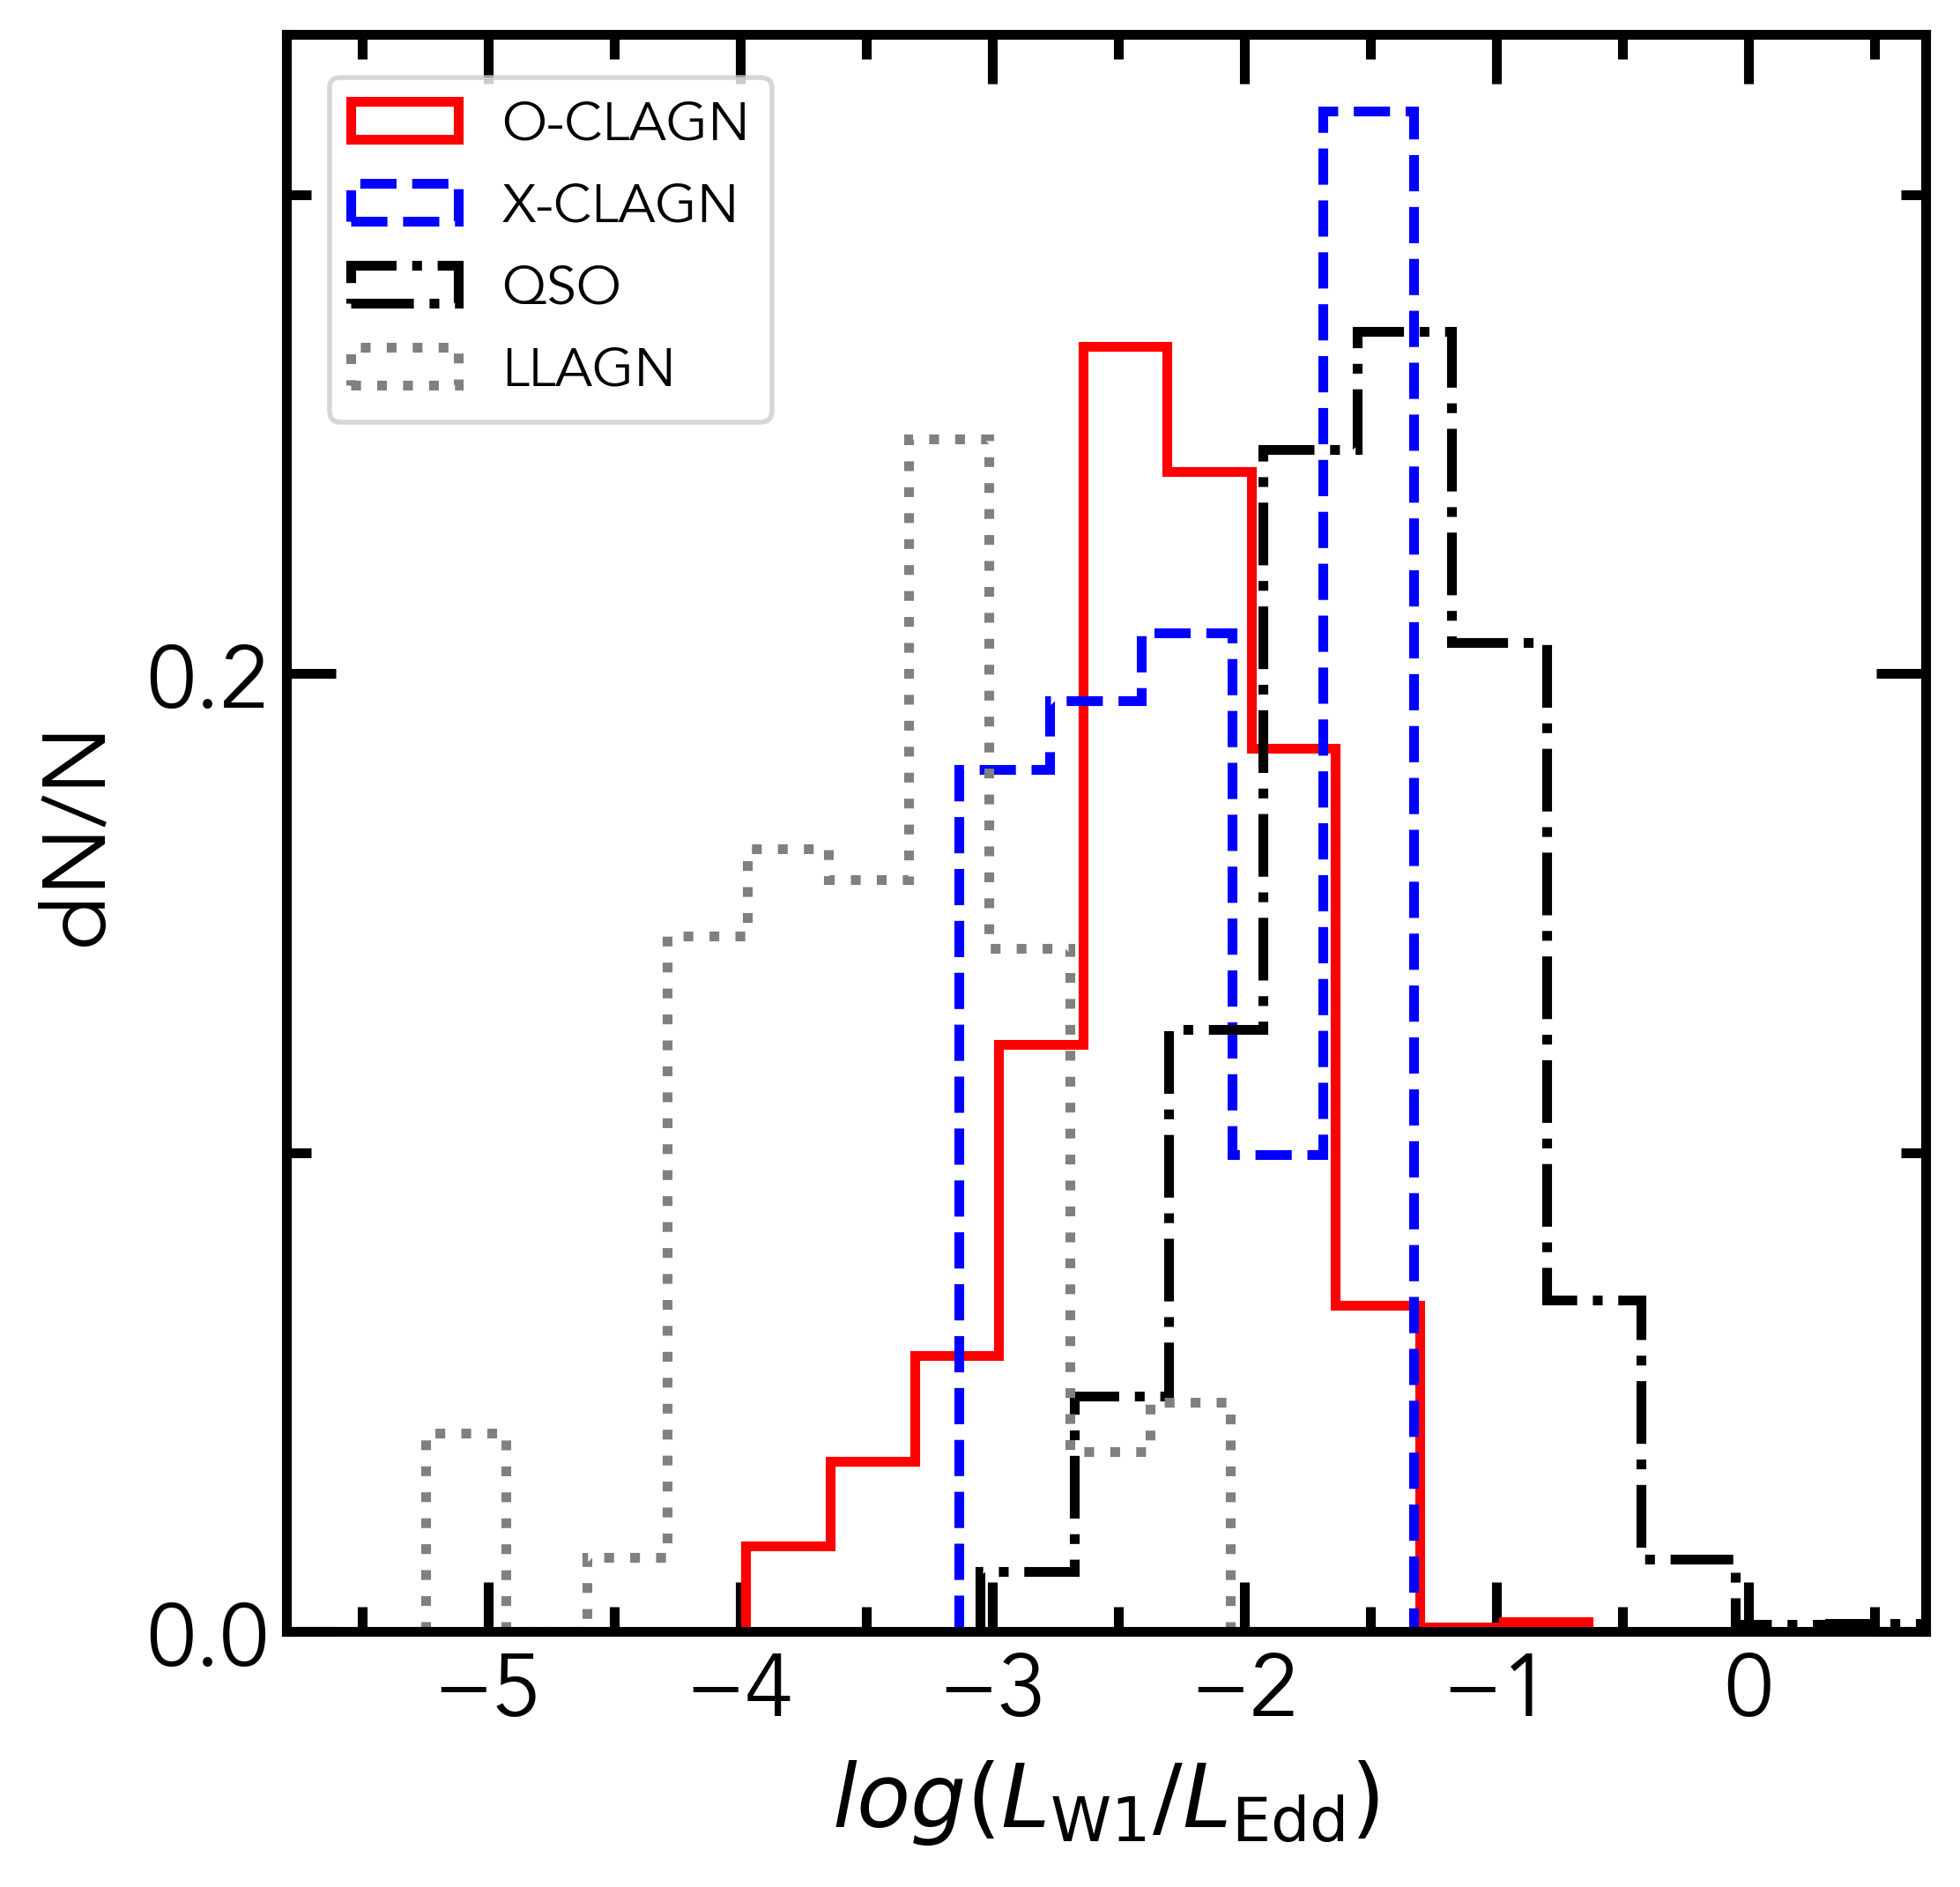
\includegraphics[width=0.45\textwidth]{pic/WISE_LW1_Ledd_hist_rebin_OX.png}
    \caption{Distribution of the Eddington-scaled W1 band luminosity re-binned in each visit for LLAGNs\citep{2009MNRAS.399..349G}, CLAGNs and QSOs \citep{2007ApJ...667..131G}. }
    \label{fig:distribution_ledd}
\end{figure}

\begin{figure}
\centering
	% To include a figure from a file named example.*
	% Allowable file formats are eps or ps if compiling using latex
	% or pdf, png, jpg if compiling using pdflatex
	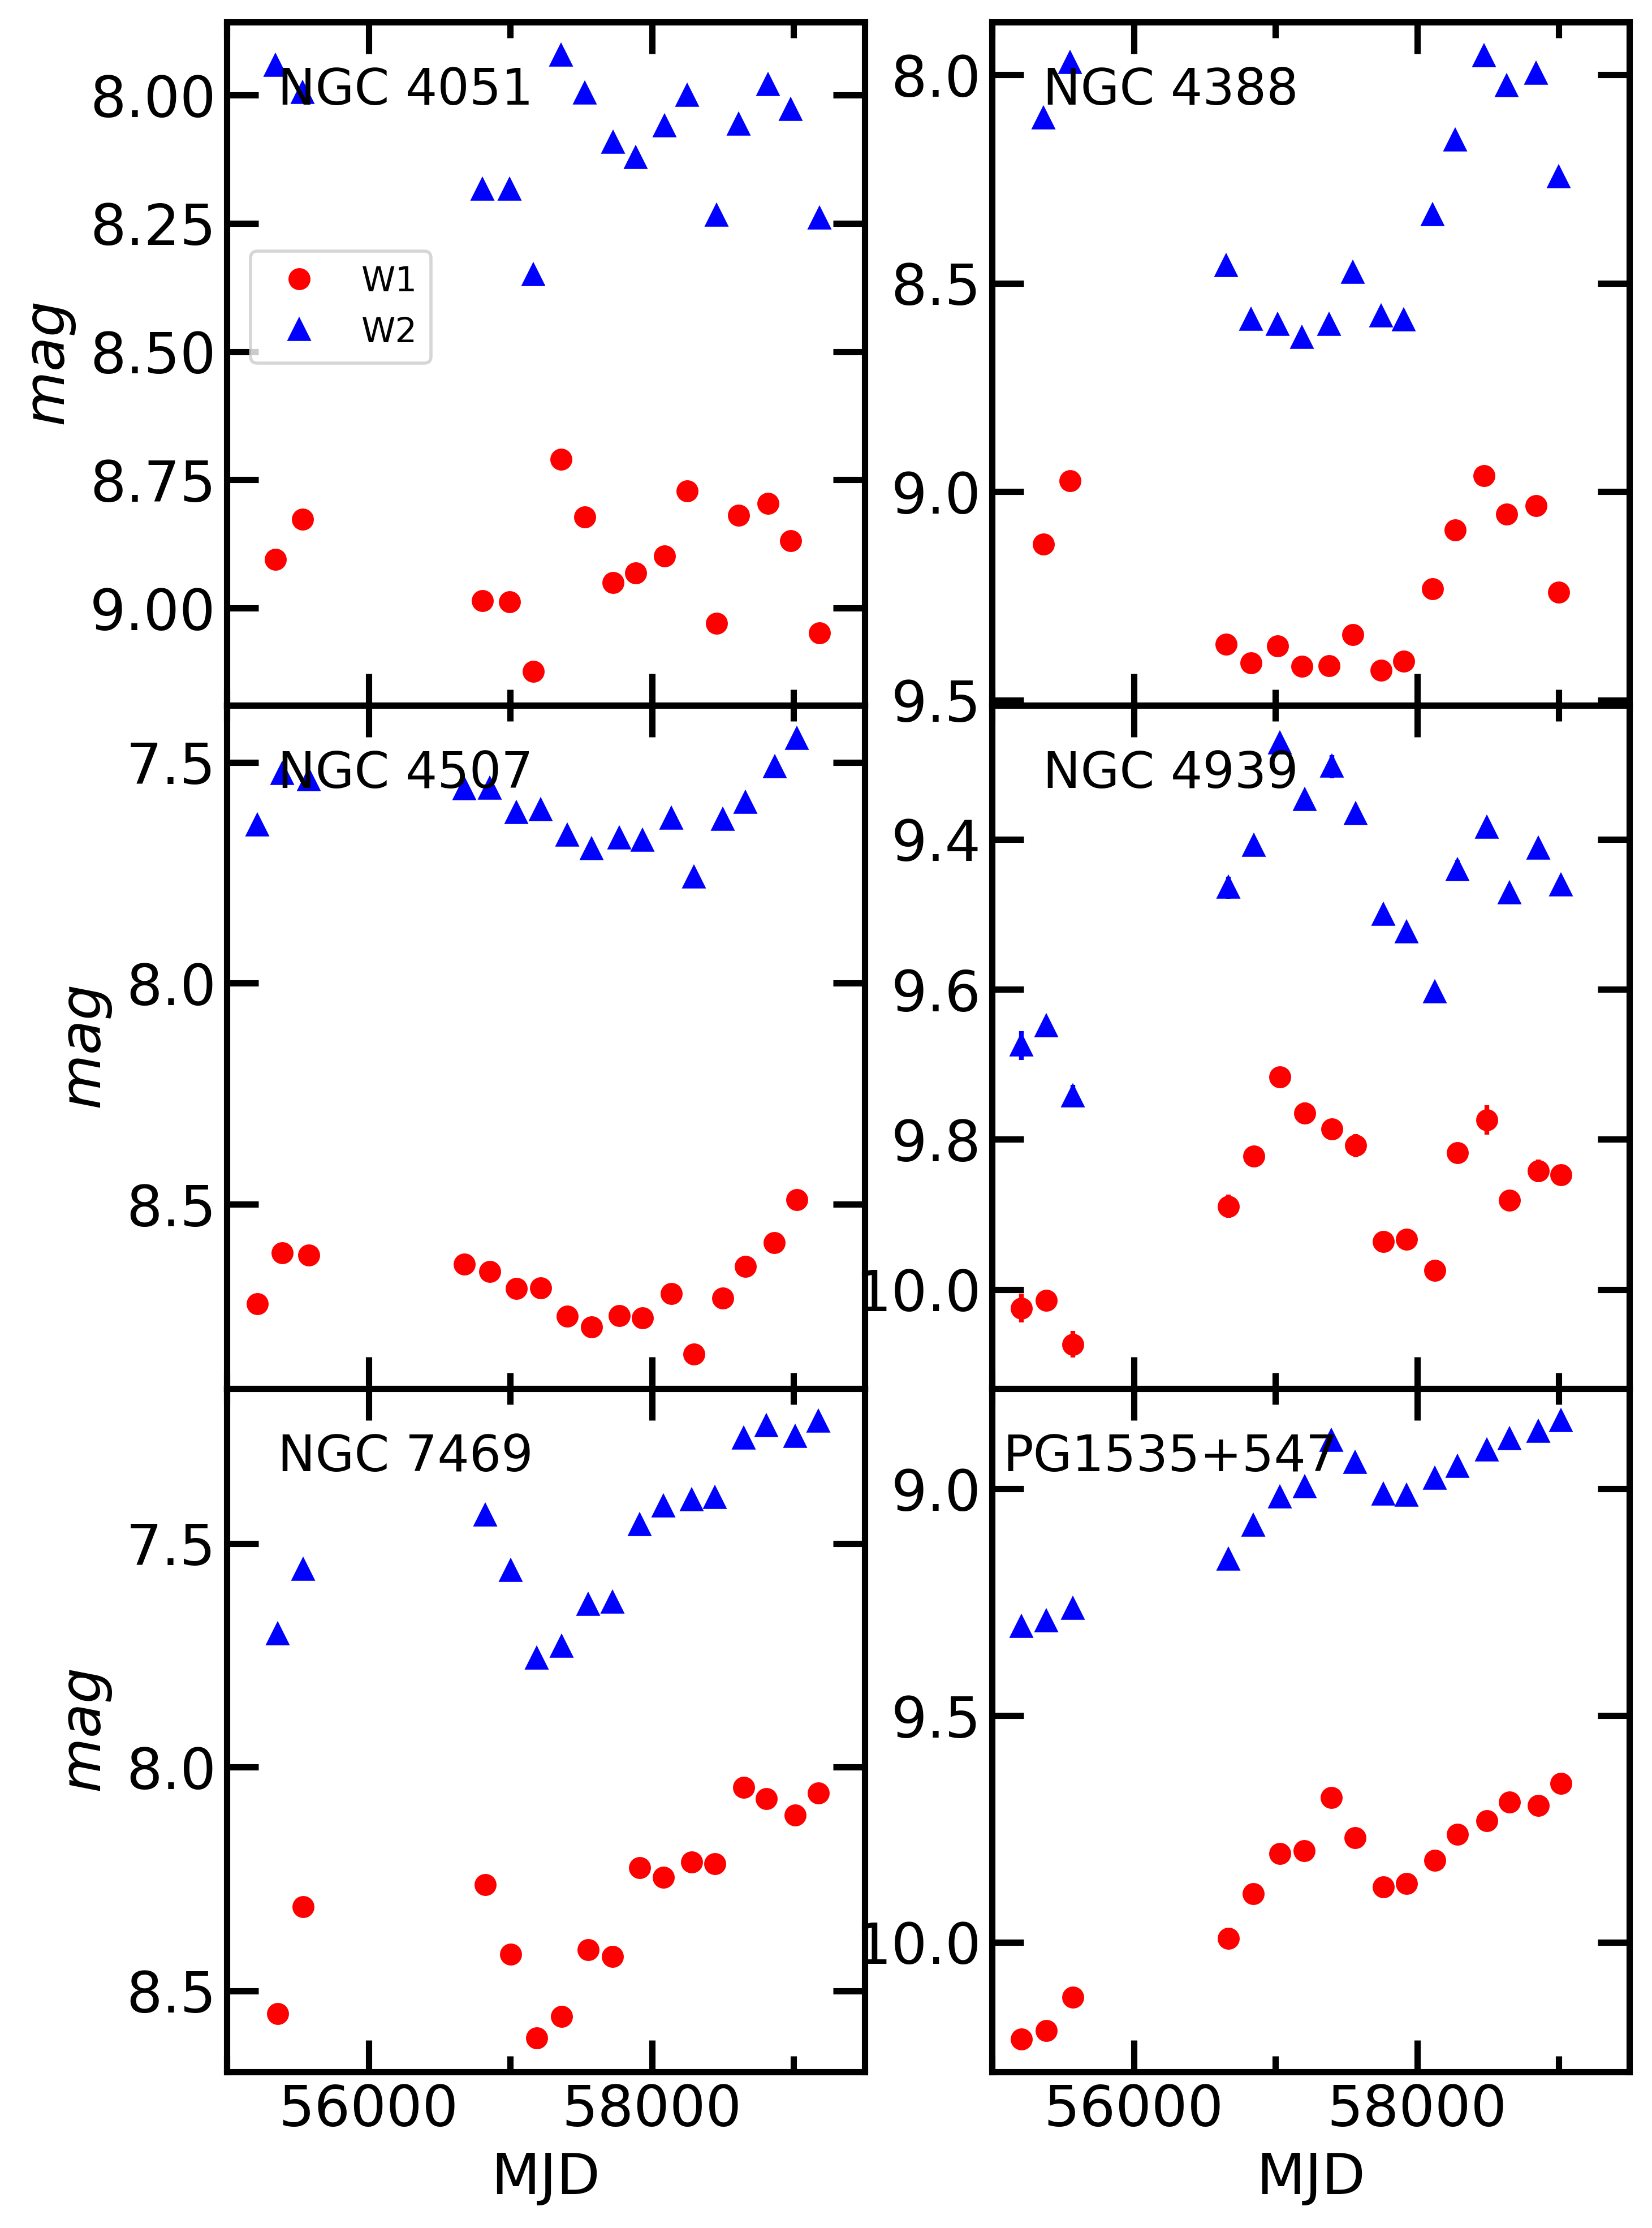
\includegraphics[width=0.6\textwidth]{pic/wisename_varX.png}
    \caption{{\it WISE} averaged light curves of highly variable X-ray CLAGNs with $\Delta\,W1$ more than $0.3$ mag. The errors are calculated by error propagation method. }
    \label{fig:X-CLAGN-lc}
\end{figure}






%We present the correlation between MIR $W$1 band variability $\sigma_{m W1}$ and mean Eddington scaled $W$1 luminosity $L_\mathrm{W1}/L_\mathrm{Edd}$\, and the distribution of $\sigma_{m W1}$ in \autoref{fig:var_ledd_hist}. The MIR luminosity is estimated from AB magnitude for $W1$ (\texttt{w1mpro} and \texttt{w1mpro\_ep}) and $W2$ (\texttt{w2mpro} and \texttt{w2mpro\_ep}) converted from Vega magnitude through $m_{\rm AB} = m_{\rm Vega} + \Delta m$, where $\Delta m$ are 2.699 and 3.339 for $W1$ and $W2$ bands, respectively. For comparison, we also plot a sample of quiescent LLAGNs from \citet{2009MNRAS.399..349G} with several sources which are classified as CLAGNs excluded and luminous QSOs from \citet{2007ApJ...667..131G}. 49 LLAGNs and 762 QSOs with at least 10 data points of \textit{NEOWISE} are included. The MIR variability of optical CLAGNs are significant higher than that of X-ray CLAGNs, LLAGNs and QSOs. We plot the correlation between mean MIR color ($W1$-$W2$) and mean $L_\mathrm{W1}/L_\mathrm{Edd}$\, and the distribution of mean $W1$-$W2$ in \autoref{fig:color_ledd}. The distribution of Eddington-scaled $W$1 luminosity ($L_\mathrm{W1}/L_\mathrm{Edd}$) from the re-binned $W$1 data is shown in \autoref{fig:distribution_ledd}.  The mean log$L_\mathrm{W1}/L_\mathrm{Edd}$\, of $-2.33$ for CLAGNs corresponds to $\sim 0.47$ per cent Eddington scaled $W$1 luminosity. Optical CLAGNs show significant higher MIR variability, slightly lower Eddington luminosity ratio, and lower $W1$-$W2$ than X-ray CLAGNs. The MIR variability, mean color, and mean luminosity for LLAGNs, CLAGNs, and QSOs samples are presented in \autoref{table_MIR_var_cor_lum}. The source information of CLAGNs is summarized in \autoref{source}. 


%The maximum variation magnitude $\Delta\,W1$ and $\Delta\,W2$ are estimated from the averaged light curve combining \textit{AllWISE} and \textit{NEOWISE} data. We find that the majority (59/70) of CLAGNs change more than $0.3$ mag for $\Delta\,W1$. And 6 of them are X-ray CLAGNs (NGC 4051, NGC 4388, NGC 4507, NGC 4939, NGC 7469, and PG 1535+547). The {\it WISE} light curves for those extreme variable sources are shown in \autoref{fig:X-CLAGN-lc}.  

%We average the {\it WISE} magnitude for each visit per half year. The errors are calculated by error propagation method.  The maximum variation magnitude $\Delta\,W1$ and $\Delta\,W2$ are estimated from the averaged light curve combining \textit{AllWISE} and \textit{NEOWISE} data. We find that the majority (59/70) of CLAGNs change more than $0.3$ mag for $\Delta\,W1$. And 6 of them are X-ray CLAGNs (NGC 4051, NGC 4388, NGC 4507, NGC 4939, NGC 7469, and PG 1535+547). The {\it WISE} light curves for those extreme variable sources are shown in \autoref{fig:X-CLAGN-lc}.  


\begin{figure}
\centering
	% To include a figure from a file named example.*
	% Allowable file formats are eps or ps if compiling using latex
	% or pdf, png, jpg if compiling using pdflatex
	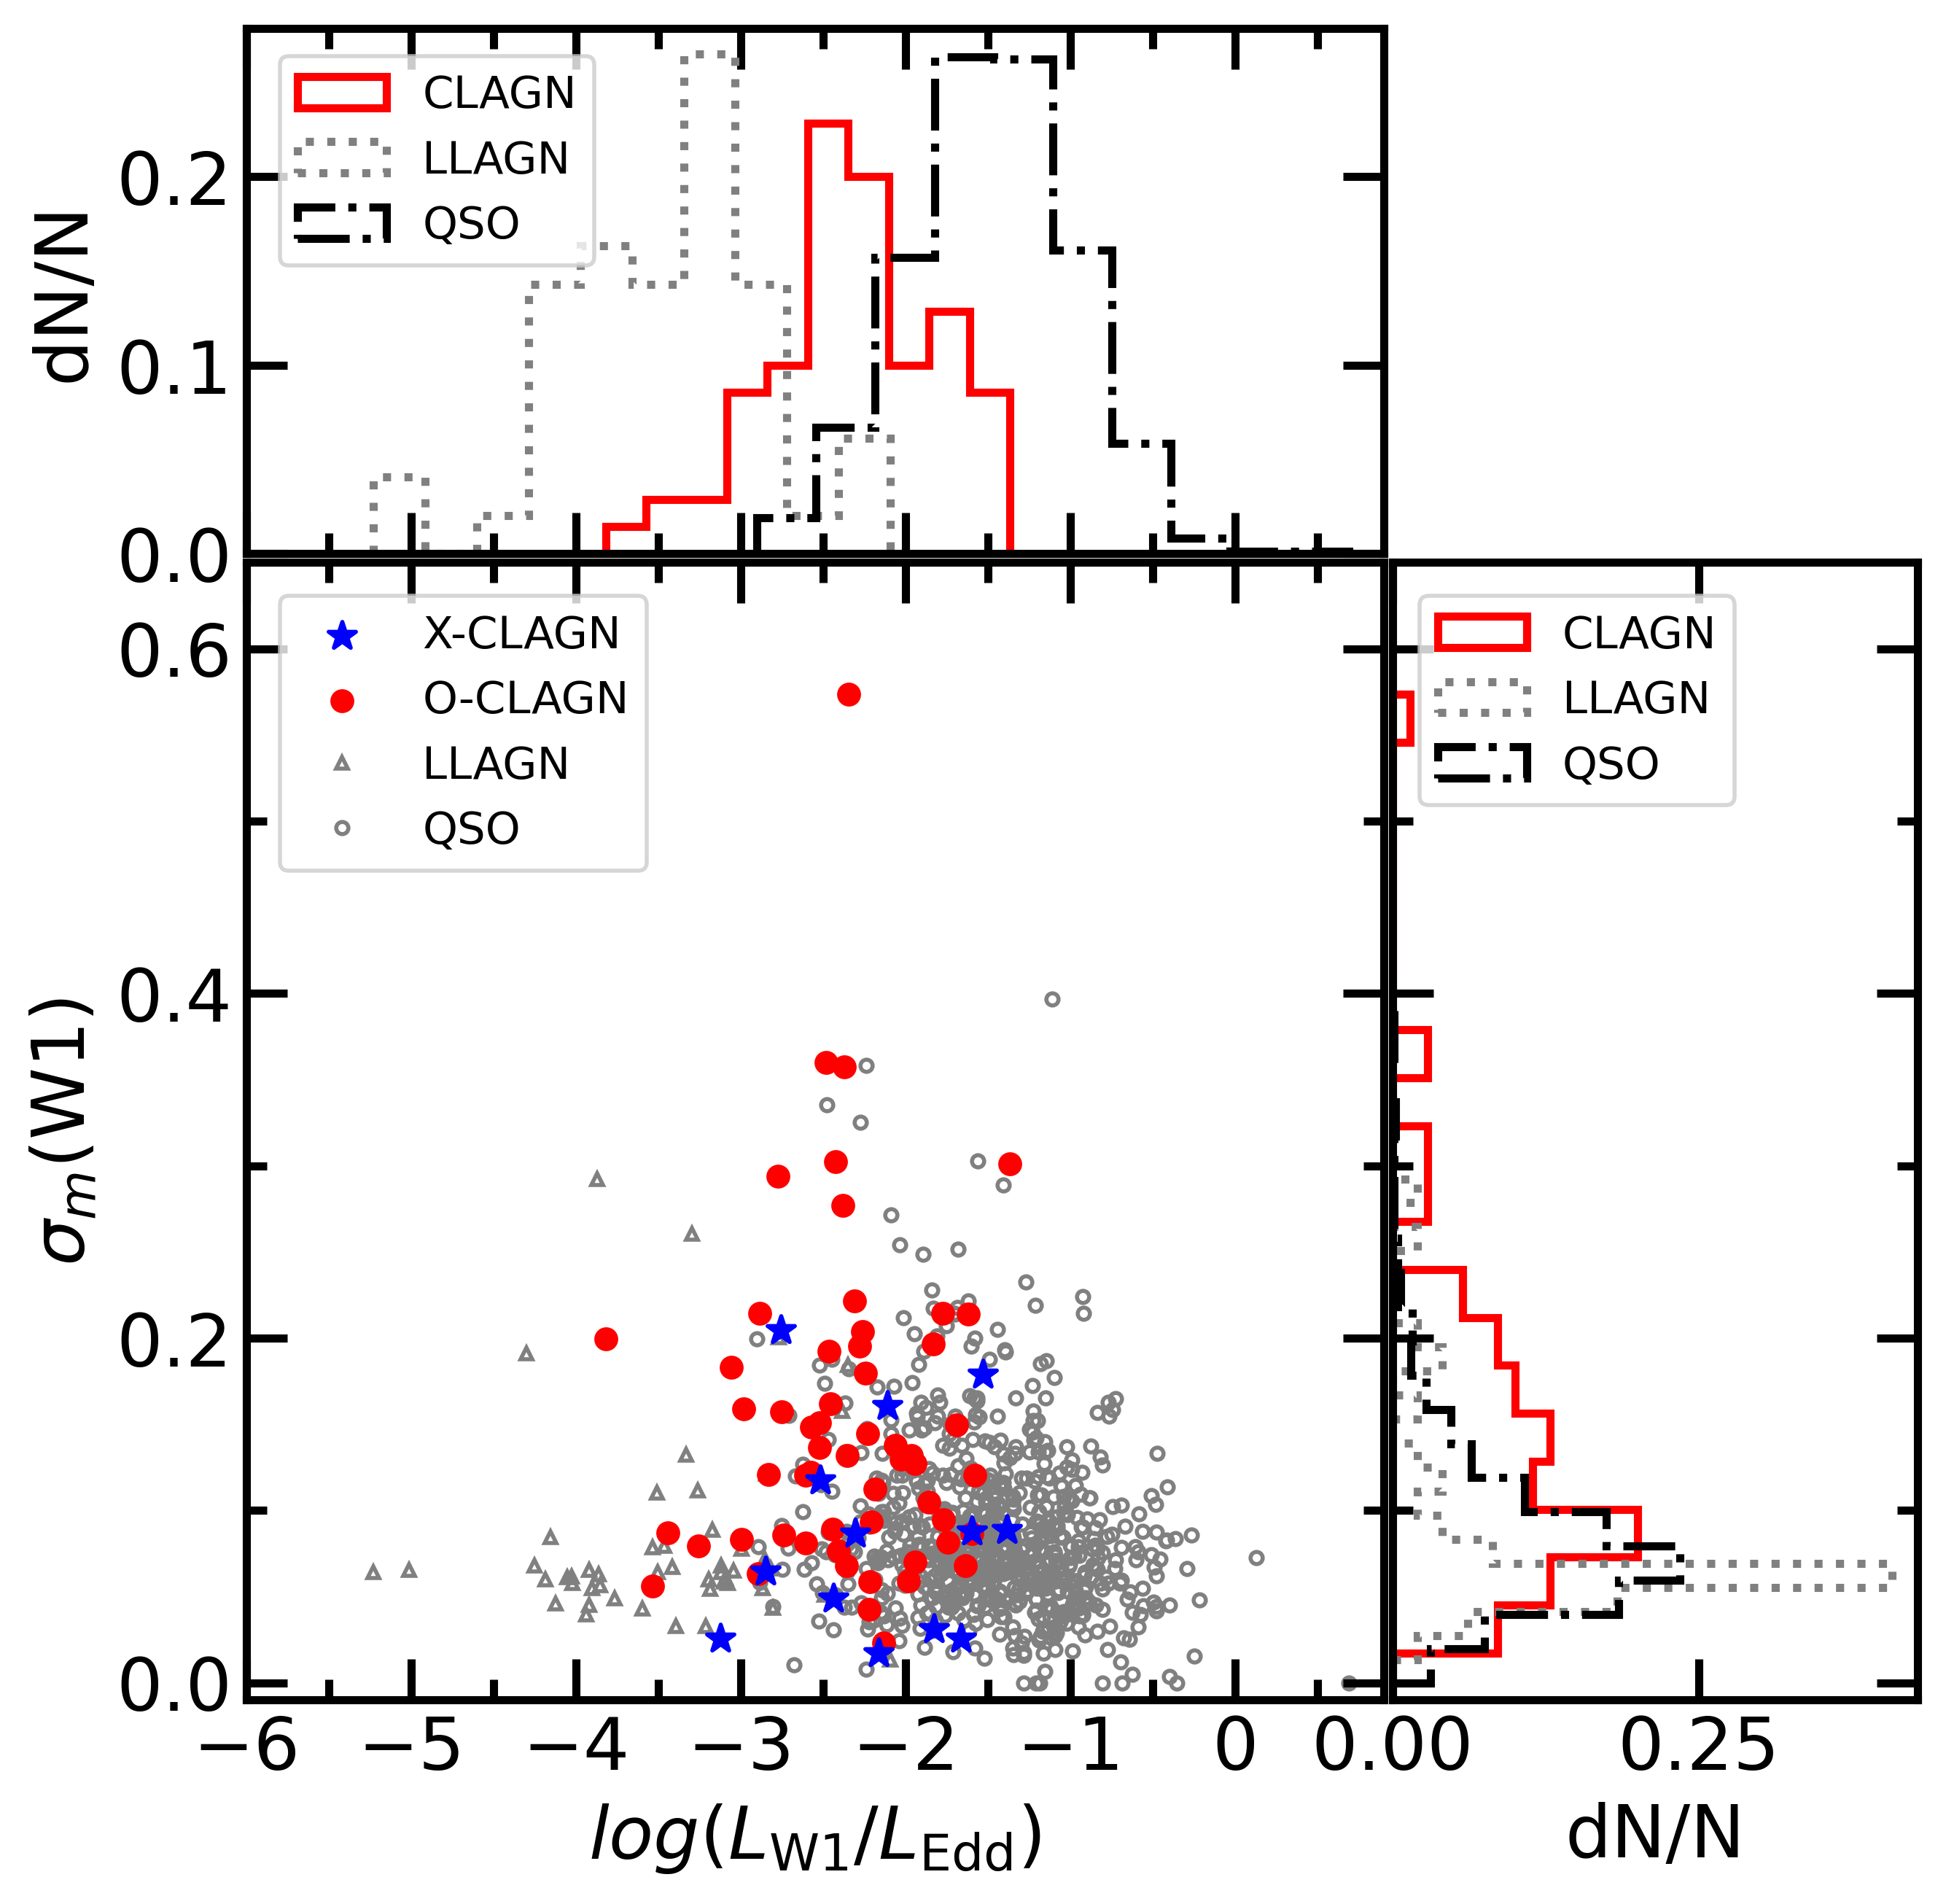
\includegraphics[width=0.45\textwidth]{WISE_var_LW1_Ledd_hist.png}
    \caption{Distribution of the variability of W1 band and its correlation with the mean Eddington-scaled W1 band luminosity for LLAGNs \citep{2009MNRAS.399..349G}, CLAGNs and QSOs \citep{2007ApJ...667..131G}. }
    \label{fig:var_ledd_hist}
\end{figure}


\begin{figure}
\centering
	% To include a figure from a file named example.*
	% Allowable file formats are eps or ps if compiling using latex
	% or pdf, png, jpg if compiling using pdflatex
	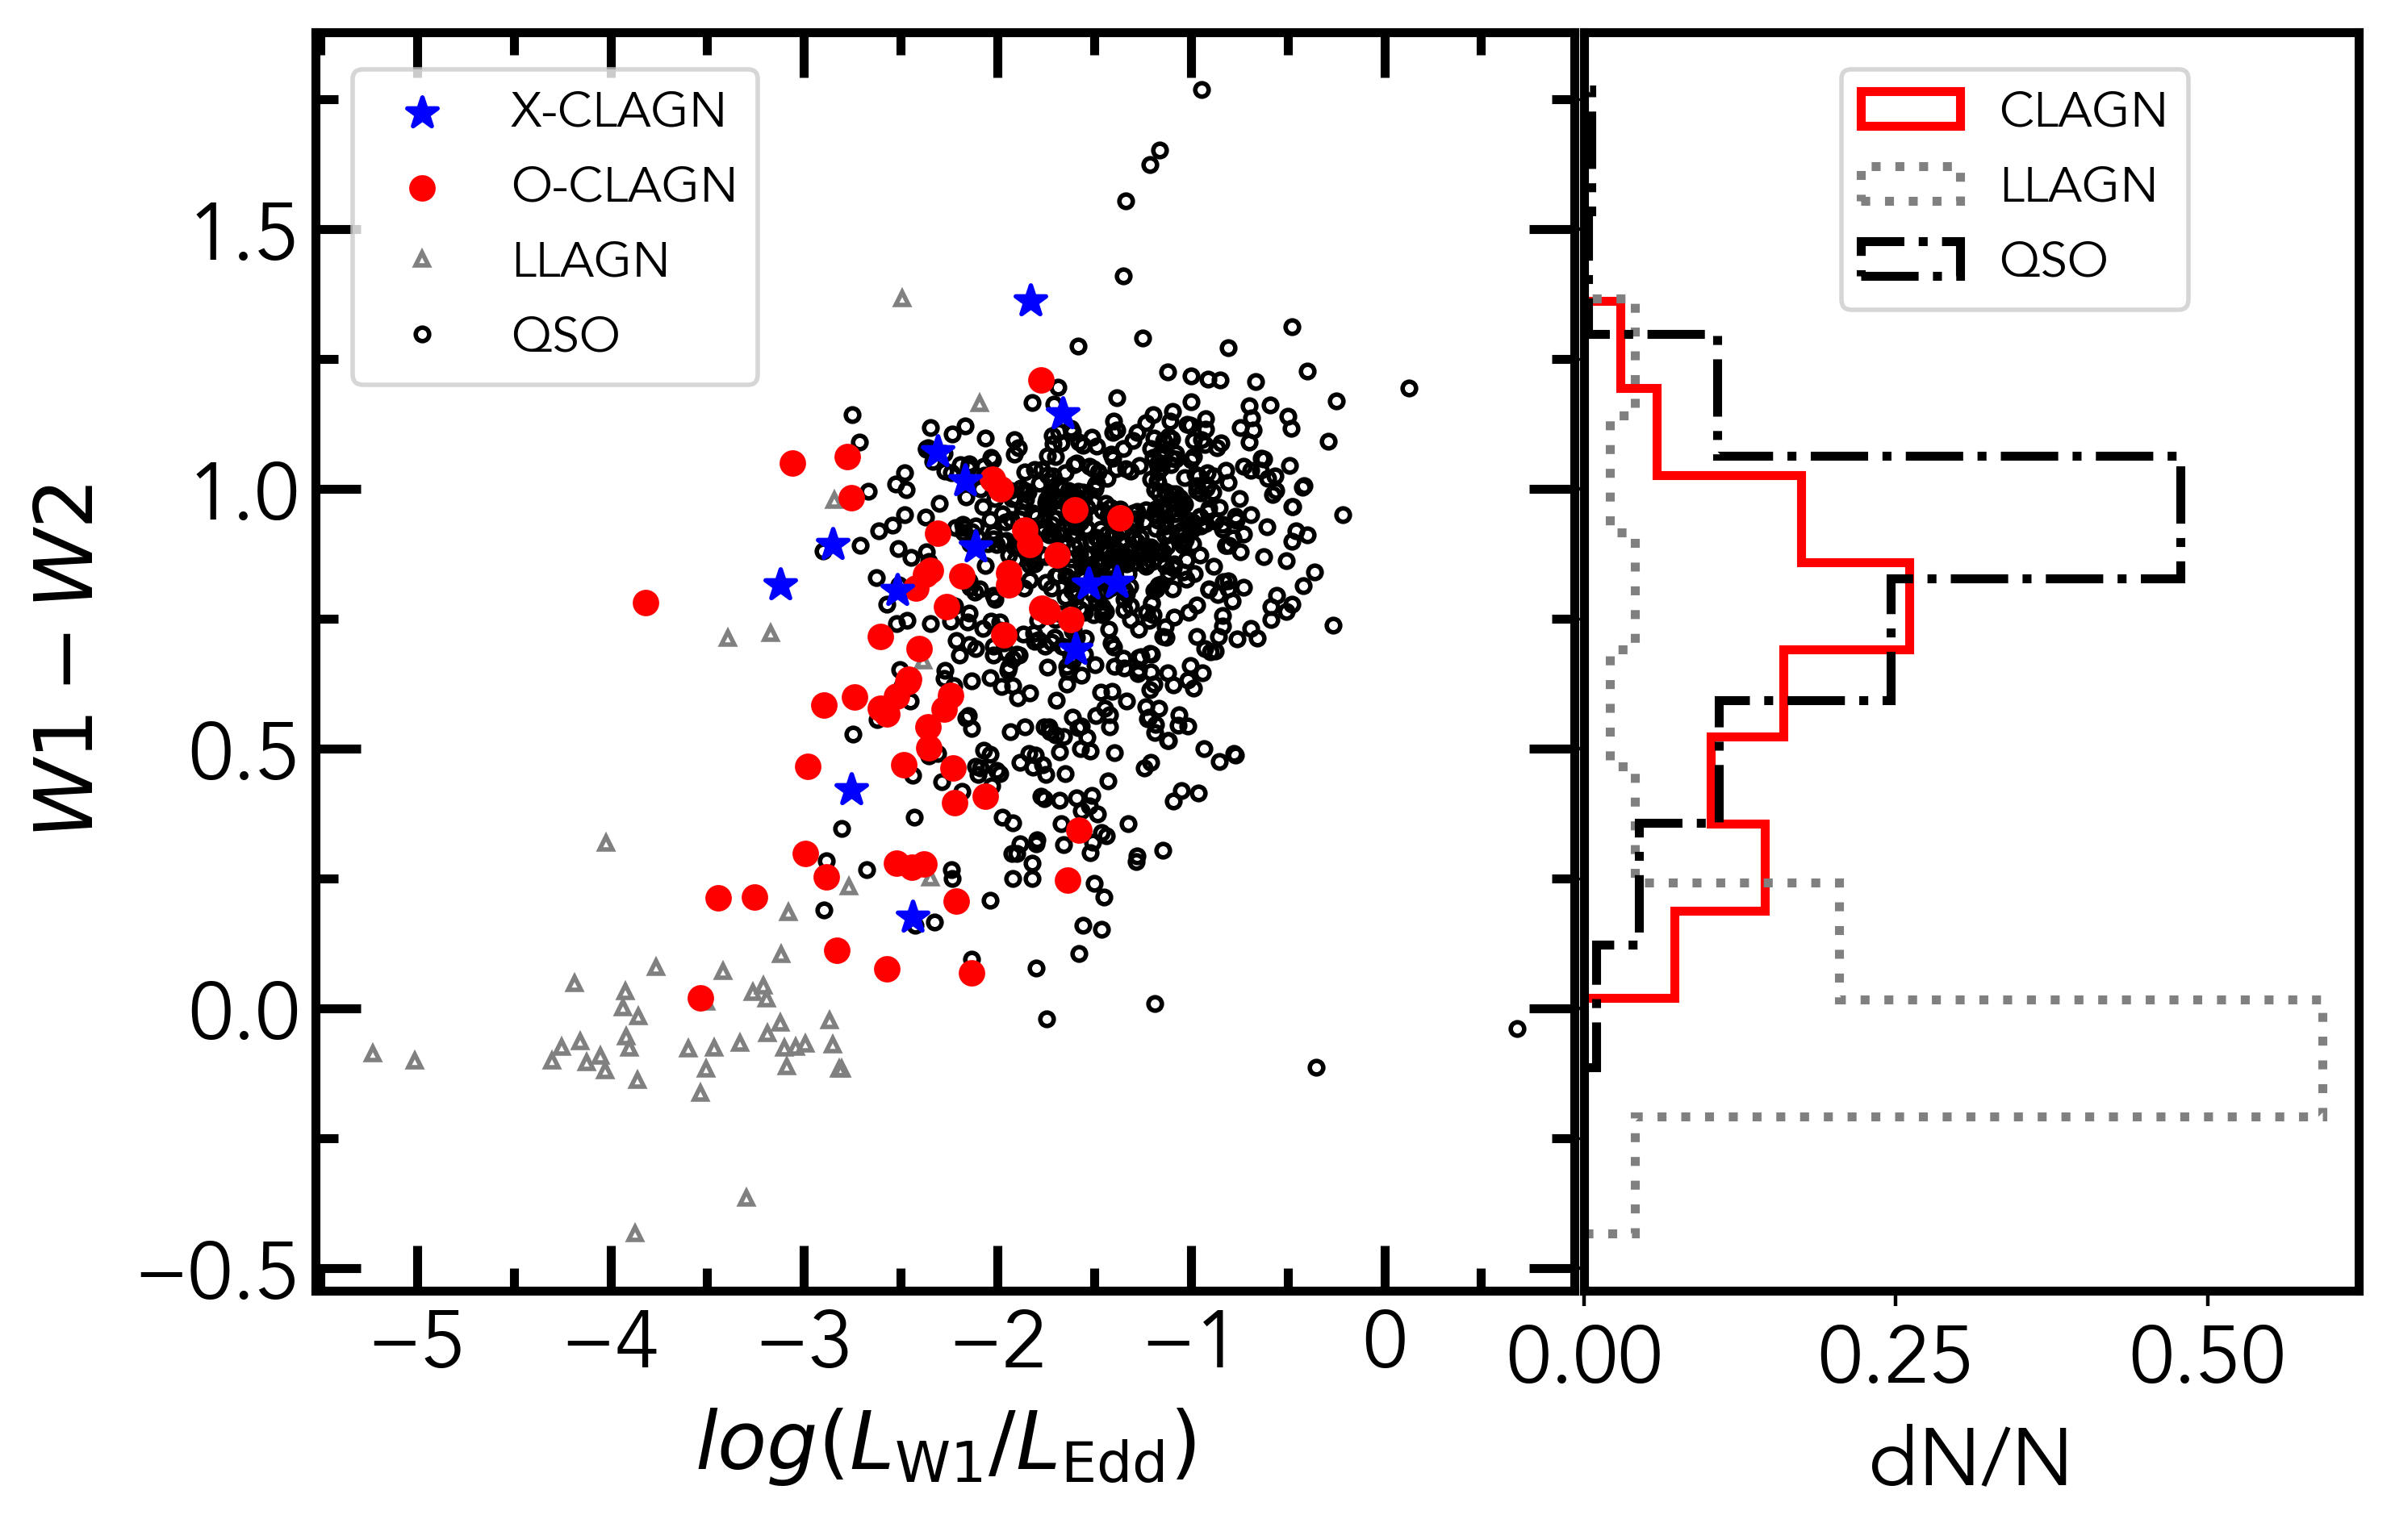
\includegraphics[width=0.45\textwidth]{pic/WISE_W1-W2_LW1_Ledd_hist.png}
    \caption{Distribution of the mean $W1-W2$ color and its correlation with the mean Eddington-scaled W1 band luminosity for LLAGNs\citep{2009MNRAS.399..349G}, CLAGNs and QSOs \citep{2007ApJ...667..131G}. }
    \label{fig:color_ledd}
\end{figure}

\begin{table}
 \caption{MIR variability, color, and Eddingtonr ratio for LLAGNs, CLAGNs, and QSOs.
}
 \label{table_MIR_var_cor_lum}
 \begin{center}
 \begin{tabular}{lccccc}
 \hline\hline
Sample             & LLAGN &   \multicolumn{3}{c}{CLAGN}        & QSO  \\ 
                   &        &   O & X   & All-CLAGN         &       \\ \hline
$\sigma_{m W1}$    &  0.083      & 0.153    &  0.088  &   0.140   &   0.088  \\ 
$\sigma_{m W2}$    &  0.065      &   0.166 &  0.083   &    0.150  &   0.080    \\ 
$<W1-W2>$          &   0.08      &  0.61   & 0.84      &    0.65    &   0.83   \\ 
$<\mathrm{log} L_\mathrm{W1}/L_\mathrm{bol}>$ & -3.46  &  -2.36  &  -2.18   &  -2.33   &  -1.48\\ 
$<\mathrm{log} L_\mathrm{W2}/L_\mathrm{bol}>$ & -3.81  &   -2.5   &  -2.23   &  -2.45   &   -1.53  \\ 
\hline\hline
\end{tabular}
\end{center}
\end{table}



\section{Dust reverberation mapping in CLAGNs}\label{sec:tau-L}
The continued observations of {\it WISE}, combined with several ground-based optical transient surveys (e.g., ASAS-SN, PTF, etc.) and space-telescope observations (e.g., \swift\,), offer a good opportunity to explore the possible dust structures in these CLAGNs. We adopt the V band data from the ASAS-SN \citep[All-sky Automated Survey for Supernovae,][]{2014ApJ...788...48S,2017PASP..129j4502K,2019MNRAS.485..961J} and \uvot\, and MIR $W1$ band data from {\it WISE} to estimate the dust echo time lag ($\tau_{W1}$) for {\color{red}CLAGNs with strong MIR variations and good optical-band monitoring}. We use the interpolation cross-correlation function \citep[ICCF;][]{1998PASP..110..660P,2018ascl.soft05032S} in a range of 0--400 days for the first attempt to estimate the dust echo time lag ($\tau$) and then further limited the range according to the posterior of $\tau$. The interpolation time steps of 5 days are applied to both optical V band and $W1$ band light curves. The flux randomization and random subset selection methods are employed with 50000 realizations in the Monte Carlo simulation to estimate the centroid time lag and the uncertainties\footnote{The code \texttt{pyCCF} is available in \url{http://ascl.net/code/v/1868}}. We also use {\sc javelin} algorithm to further test the results of the ICCF method, where {\sc javelin} algorithm fits the light curves using a damped random walk (DRW) model with amplitude and time scale of the variability. A top-hat transfer function (TF) is convolved with the driving light curve and the best-fit model parameters such as time lag $\tau$ are found through the Markov Chain Monte Carlo method. We restrict the lag we search in a range in 0-400 days and width range in 0-400 days in the first attempt. We get time lag measurements of 10 sources with long-term and high-cadence observations, which are described in detail in \autoref{lag_analysis}. We adopt the time lags from the ICCF method as primary results in the following analysis, where the time lags are listed in \autoref{table_lag}. 

%(see Appendix for more details for the data of each source)

To explore the possible correlation between dust-reverberation time lag ($\tau_{W1}$) and bolometric luminosity ($L_\mathrm{bol}$), we estimate the bolometric luminosities of CLAGNs from the X-ray luminosity through a bolometric correction of $L_{\mathrm{bol}}=8 \times L_{\mathrm{14-195 keV }}$ \citep[e.g.,][]{2009MNRAS.392.1124V}, where the X-ray data are obtained from the 105-Month Swift-BAT All-sky Hard X-Ray Survey reported in \citet{2018ApJS..235....4O}. {\color{red}The bolometric luminosity of PG 1535+547 we adopt is $\sim 1.4\times \, 10^{45} erg\, s^{-1}$ estimated from [O~{\small III}] line by empirical correlation of \citet{2006ApJ...653..137Z}, since PG 1535+547 is not included in the above \bat\, survey}. The correlation between $\tau_{W1}$ and $L_\mathrm{bol}$ for CLAGNs is shown in \autoref{fig:tau_L}. It can be found that the brighter CLAGNs have longer time delays. We apply a Spearman's rank correlation coefficient to test the correlation between log$\tau$ and log$L_{bol}$ for CLAGNs, which yields a coefficient of $0.97$ ($p=5.2\times10^{-6}$). We then use UltraNest\footnote{\url{https://johannesbuchner.github.io/UltraNest/}} package \citep{2021JOSS....6.3001B} to fit the linear log$\tau$-log($L_{bol}/10^{11} L_{\odot}$) correlation of CLAGNs with errors considered. The fitting result shows a slope of $0.29^{+0.04}_{-0.03}$ with a scatter of $0.02^{+0.04}_{-0.01}$ (solid line). The slope ($0.29^{+0.04}_{-0.03}$) of the $\tau$-$L_{bol}$ correlation is slightly lower than the slope ($0.47 \pm 0.06$) from the fitting of PG quasars (dashed line) in \citet[][]{2019ApJ...886...33L}.


%The bolometric luminosity of NGC 1566 is $\sim 8.7\times \, 10^{42} erg\, s^{-1}$ (method??).
%This is consistent with the result ( 0.09--7.11 $\times \, 10^{43} erg\, s^{-1}$) from X-ray luminosity \citep[see][]{2021MNRAS.507..687J} through a bolometric correction of $L_{bol}=20 L_{\mathrm{2-20 keV}}$ \citep[e.g.,][]{2009MNRAS.392.1124V}. 



\begin{figure}
\centering
	% To include a figure from a file named example.*
	% Allowable file formats are eps or ps if compiling using latex
	% or pdf, png, jpg if compiling using pdflatex
	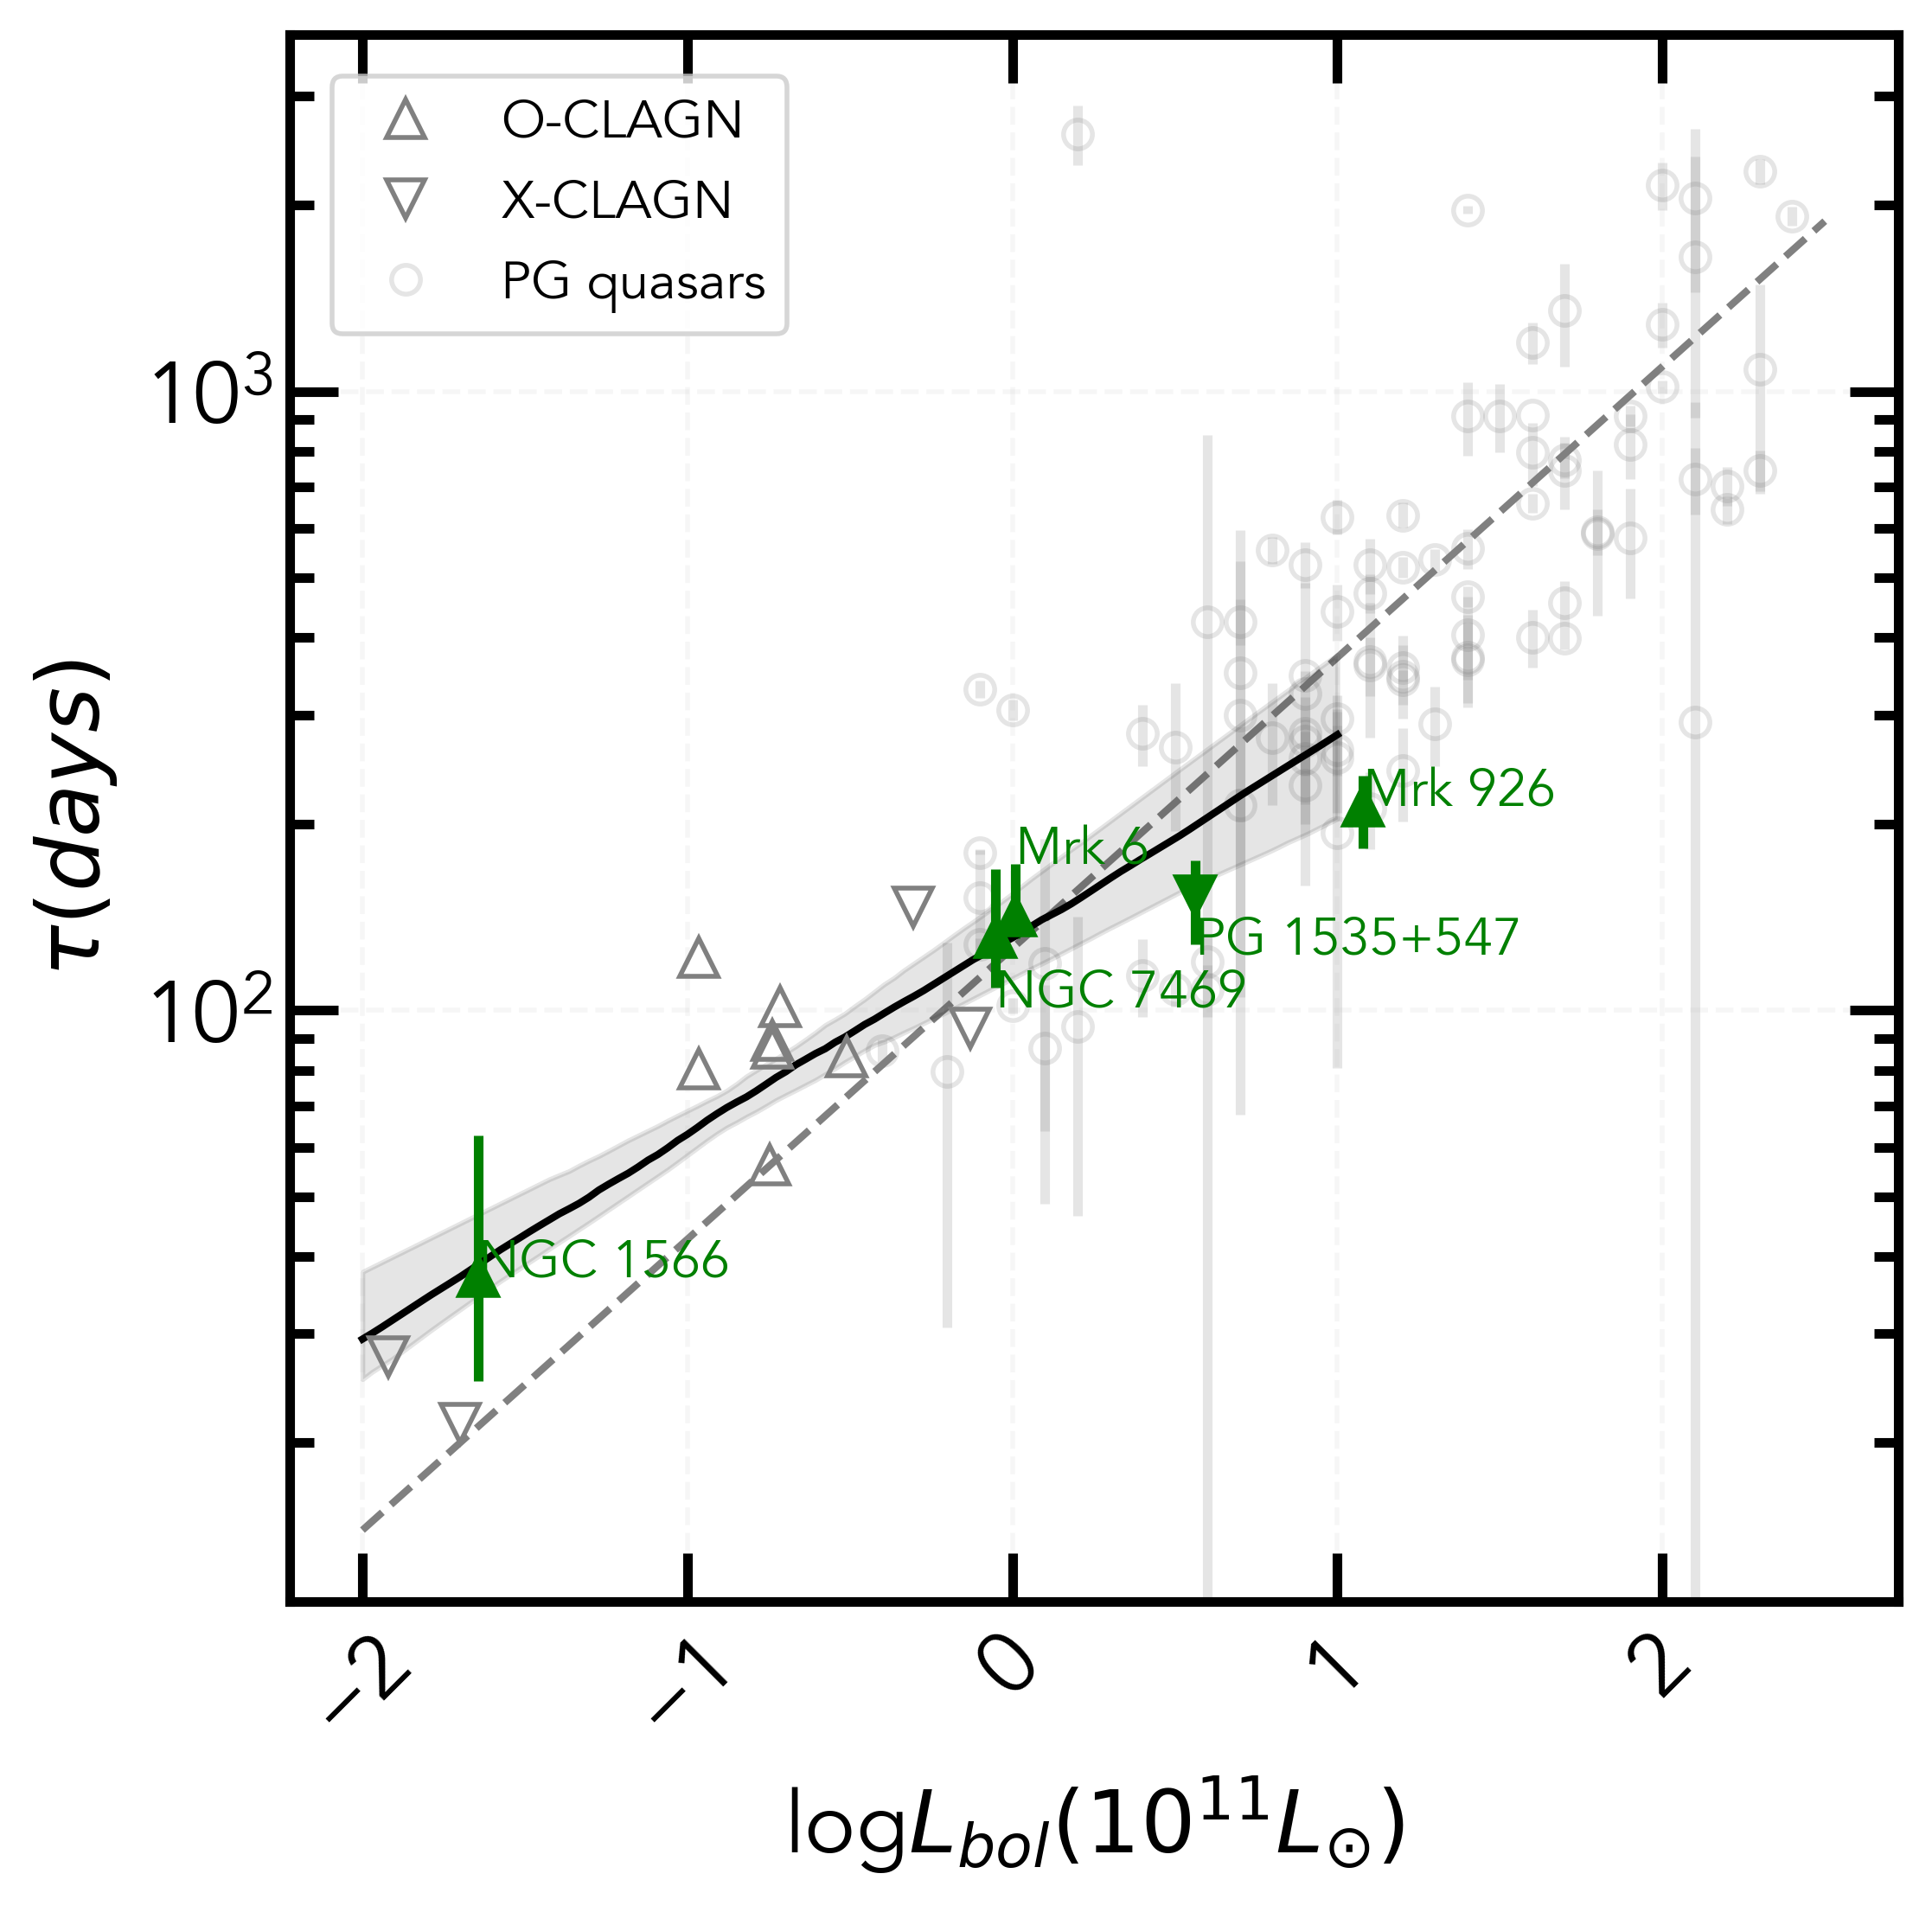
\includegraphics[width=0.45\textwidth]{tau_L_correlation_clagn.png}
    \caption{$\tau$-L correlation for CLAGNs, where $\tau$ is time lag between V band and $W$1 band and L is bolometric luminosity. Grey circles represent PG quasars \citep{2019ApJ...886...33L} for comparison. The dashed line repserent the best fitting of $\tau$-L correlation for PG quasars in \citet{2019ApJ...886...33L}. The straight line is the best fitting for CLAGNs with a scatter in the shadow region.} 
    \label{fig:tau_L}
\end{figure}


\begin{table}
 \caption{Dust reverberation time lag of CLAGNs.
}
 \label{table_lag}
 \begin{center}
 \begin{tabular}{lcccc}
 \hline\hline
Name & log($L_{bol}$) & $\tau$~(days) &Type \\ \hline 
Mrk 590 & 44.13 & $57.9^{+17.8}_{-20.0}$ & O \\
Mrk 6 & 44.59 & $142.1^{+30.0}_{-11.5}$ & O \\
Mrk 926 & 45.66 & $213.8^{+25.3}_{-31.0}$ & O \\
NGC 1566 & 42.94 & $37.1^{+25.7}_{-11.9}$ & O \\
NGC 3516 & 44.19 & $91.1^{+64.0}_{-31.4}$ & O \\
NGC 4051 & 42.61 & $22.3^{+10.4}_{-10.0}$ & X \\
NGC 4151 & 44.08 & $74.4^{+40.8}_{-19.5}$ & O \\
NGC 5548 & 44.66 & $131.2^{+18.6}_{-32.2}$ & O \\
NGC 7469 & 44.53 & $131.2^{+37.9}_{-22.4}$ & X \\
PG 1535+547 & 45.15 & $153.2^{+21.2}_{-25.3}$ & X \\
\hline\hline
\end{tabular}
\end{center}
Note. The table lists source name, bolometric luminosity, dust reverberation time lag between V band and $W$1 band, CLAGN types (``O'' for optical CLAGN and ``X'' for X-ray CLAGN). 
\end{table}


%\begin{figure}
\centering
	% To include a figure from a file named example.*
	% Allowable file formats are eps or ps if compiling using latex
	% or pdf, png, jpg if compiling using pdflatex
	\includegraphics[width=0.5\textwidth]{tau_L_correlation_type.png}
    \caption{$\tau$-L correlation for CLAGNs and quasars, where $\tau$ is time lag between V band and $W$1 band and L is bolometric luminosity. Grey circles represent PG quasars \citep{2019ApJ...886...33L}. The grey dashed line repserent the best fitting of $\tau$-L correlation for PG quasars with a slope of $\sim$ 0.47 in \citet{2019ApJ...886...33L}.
    Stars represent Type 1 AGN \citep[][]{2014ApJ...788..159K,2019ApJ...886...33L}. The time lags for Type 1s are scaled from $\tau_\mathrm{K}$ to $\tau_\mathrm{W1}$ by multiplying a factor of 5/3 according to \citet[][]{2019ApJ...886...33L}. Square represents the type 2 AGN NGC 2110 for X-ray and MIR time lag \citep[see ][]{2020MNRAS.495.2921N}. The black straight line represents the best-fitting for Type 1s, Type 2s, and CLAGNs, with a slope of $\sim$ 0.36. The red dashed lines represent the scatter of $\sim$0.17 dex.  }
    \label{fig:tau_L}. 
\end{figure}


\begin{table}
 \caption{Dust reverberation time lag of CLAGNs.
}
 \label{table_lag}
 \begin{center}
 \begin{tabular}{lccccc}
 \hline\hline
Name & log($L_{bol}/L_{\odot}$) & $\tau$~(days) &Type  & references\\ \hline 
NGC 1566 & 9.91 & $37.1^{+25.7}_{-11.9}$ & O & This work \\
Mrk 6 & 11.01 & $142.1^{+30.0}_{-11.5}$ & O & This work \\
Mrk 926 & 12.08 & $213.8^{+25.3}_{-31.0}$ & O & This work \\
PG 1535+547 & 11.56 & $153.2^{+21.2}_{-25.3}$ & X & This work \\
NGC 2110 & 10.95 & $153.2^{+21.2}_{-25.3}$ & Type 2 & \citet{2020MNRAS.495.2921N} \\
Mrk 335 & 11.03 & $ 167.1 \pm 5.60$ & Type 1 & \citet{2014ApJ...788..159K} \\
Mrk 590 & 10.25 & $ 33.8 \pm 4.20$ & O & \citet{2014ApJ...788..159K} \\
IRAS 03450+0055 & 11.34 & $ 158.3 \pm 5.40$ & Type 1 & \citet{2014ApJ...788..159K} \\
Akn 120 & 11.67 & $ 140.9 \pm 17.20$ & Type 1 & \citet{2014ApJ...788..159K} \\
MCG +08-11-011 & 10.88 & $ 73.5 \pm 1.40$ & Type 1 & \citet{2014ApJ...788..159K} \\
Mrk 79 & 10.77 & $ 65.6 \pm 5.00$ & Type 1 & \citet{2014ApJ...788..159K} \\
Mrk 110 & 11.03 & $ 119.7 \pm 5.50$ & Type 1 & \citet{2014ApJ...788..159K} \\
NGC 3227 & 9.60 & $ 14.6 \pm 0.70$ & Type 1 & \citet{2014ApJ...788..159K} \\
NGC 3516 & 10.03 & $ 73.1 \pm 4.00$ & O & \citet{2014ApJ...788..159K} \\
Mrk 744 & 9.23 & $ 20.0 \pm 2.20$ & Type 1 & \citet{2014ApJ...788..159K} \\
NGC 4051 & 9.08 & $ 16.5 \pm 0.60$ & X & \citet{2014ApJ...788..159K} \\
NGC 4151 & 10.03 & $ 48.3 \pm 0.50$ & O & \citet{2014ApJ...788..159K} \\
NGC 4593 & 9.95 & $ 41.6 \pm 0.90$ & Type 1 & \citet{2014ApJ...788..159K} \\
NGC 5548 & 10.29 & $ 60.9 \pm 0.30$ & O & \citet{2014ApJ...788..159K} \\
Mrk 817 & 11.12 & $ 93.0 \pm 8.90$ & Type 1 & \citet{2014ApJ...788..159K} \\
Mrk 509 & 11.63 & $ 120.7 \pm 1.80$ & Type 1 & \citet{2014ApJ...788..159K} \\
NGC 7469 & 10.69 & $ 88.0 \pm 0.60$ & X & \citet{2014ApJ...788..159K} \\
Mrk 335 & 11.17 & 137.7 & Type 1 & \citet{2019ApJ...886...33L} \\
IRAS 03450+0055 & 11.46 & 129.1 & Type 1 & \citet{2019ApJ...886...33L} \\
MCG +08-11-011 & 11.76 & 89.5 & Type 1 & \citet{2019ApJ...886...33L} \\
Mrk 79 & 10.93 & 74.6 & Type 1 & \citet{2019ApJ...886...33L} \\
Mrk 110 & 11.17 & 63.7 & Type 1 & \citet{2019ApJ...886...33L} \\
NGC 3227 & 9.85 & 7.0 & Type 1 & \citet{2019ApJ...886...33L} \\
NGC 3516 & 10.26 & 53.6 & O & \citet{2019ApJ...886...33L} \\
Mrk 744 & 9.48 & 26.6 & Type 1 & \citet{2019ApJ...886...33L} \\
NGC 4051 & 9.30 & 12.9 & X & \citet{2019ApJ...886...33L} \\
NGC 4151 & 10.26 & 52.2 & O & \citet{2019ApJ...886...33L} \\
NGC 4593 & 10.17 & 62.1 & Type 1 & \citet{2019ApJ...886...33L} \\
NGC 5548 & 10.49 & 50.5 & O & \citet{2019ApJ...886...33L} \\
Mrk 817 & 11.26 & 91.6 & Type 1 & \citet{2019ApJ...886...33L} \\
Mrk 509 & 11.71 & 122.2 & Type 1 & \citet{2019ApJ...886...33L} \\
NGC 7469 & 10.87 & 56.1 & X & \citet{2019ApJ...886...33L} \\
\hline\hline
\end{tabular}
\end{center}
Note. The table lists source name, bolometric luminosity, dust reverberation time lag, CLAGN types (``O'' for optical selected CLAGN and ``X'' for X-ray selected CLAGN) and references. The time lag for type 2 AGN NGC 2110 is between X-ray (2-20 keV) band and $W$1 band. The time lag for NGC 1566 is between V band and $W$1 band in this work. The time lags results from \citet{2014ApJ...788..159K} and \citet{2019ApJ...886...33L} are between V band and K band. 
\end{table}



\section{Conclusion and Discussion} \label{sec:dis}
 We perform an analysis on the MIR data of {\it WISE} for a sample of both X-ray and optical CLAGNs to explore the possible physical mechanism behind them. We find that the Eddington scaled MIR luminosity of CLAGNs is lower than that of QSOs but higher than that of LLAGNs. The majority of CLAGNs shows strong MIR variabilities, where the variability $\sigma_{m}$ is stronger than that of both LLAGNs and QSOs. The color of $W1-W2$ also shows a wider distribution in CLAGNs, where brighter and fainter CLAGNs are similar to QSOs and LLAGNs, respectively. The above results support that the CLAGNs most possibly stay in a transition stage. Based on the MIR and optical variability, we estimate the time delays of 10 CLAGNs, where these sources still roughly follow the $\tau_{W1}-L_\mathrm{bol}$ correlation as defined by QSOs. The dust echo in CLAGNs supports that the dust reprocessing and the large variability in both optical CLAGNs and X-ray CLAGNs are triggered by the change of accretion rate.
  
\subsection{Transition state of CLAGNs}

The study of the intrinsic physics of CLAGNs will help us to understand the nature of accretion flow and the evolution of galaxies. Furthermore, the physical mechanism for the two types of CLAGNs (optical CLAGNs and X-ray CLAGNs) is also quite unclear. Since the MIR emission is produced by dust heated by the UV radiation of the accretion disk, the MIR properties of CLAGNs will shed light on their central engine. Most of CLAGNs show strong variation in the MIR band (e.g., more than 85\% sources have maximum variation magnitude $\Delta>0.3$ in $W$1 band), which include 6 X-ray CLAGNs (totally 13). The variation suggests that most of the optical and X-ray CLAGNs cannot be simply explained by the motion of absorbing clouds moving in/out of our line of sight, where the changing look should be correlated with the variation of the accretion disk (e.g., change of disk structure, disk wind, etc). The Eddington ratio of MIR luminosity for CLAGNs just stays between QSOs and LLAGNs, where the standard accretion disk and ADAF are widely believed in QSOs and LLAGNs, respectively. The average value of $L_\mathrm{W1}/L_\mathrm{Edd} \sim $0.5\%, which roughly corresponds to $L_\mathrm{bol}/L_\mathrm{Edd}$ at several per cent by assuming a bolometric correction factor of $\sim 10$ \citep[e.g.,][]{2012MNRAS.426.2677R}. The multi-epoch observations of CLAGNs often show that they cross a critical bolometric Eddington ratio of  $L_\mathrm{bol}/L_\mathrm{Edd}\sim$1\% during their dramatic transformations \citep[e.g.,][]{2019ApJ...883...76R,2021MNRAS.508..144G,2021MNRAS.506.4188L,2021MNRAS.507..687J}, approximately where accretion state transitions are often observed to occur in X-ray binaries \citep[e.g.,][]{2008ApJ...682..212W}. We find that the CLAGNs show stronger MIR variation compared to LLAGNs and QSOs (see \autoref{fig:var_ledd_hist}), which may be triggered by the quick disk transition between SSD and ADAF at a critical accretion rate of $\sim$1\% Eddington rate. The CLAGNs will show galaxy-like MIR color (e.g., $W1-W2\leq0.5$) when the sources enter into the faint state, while they will show AGN-like MIR color (e.g., $W1-W2\geq0.5$) when the sources enter into the bright state and vice versa \citep[e.g.,][]{2012ApJ...753...30S,2013AJ....145...55Y,2017ApJ...846L...7S}. Therefore, the color distribution of CLAGNs also supports the possible disk transition in CLAGNs. 

%(MacLeod et al. 2019; Ruan et al. 2019,Liuhao,lyu etc.)
%(Stern et al. 2012; Yan et al. 2013; Sheng et al. 2017)

As the accretion rate decreases below the critical rate, the inner cold disk might transit into ADAF and the intrinsic luminosities will drop, which will reduce the ionizing photons for exciting the broad emission lines. The BLR clouds may quickly fall onto the central SMBHs when the radiation pressure suddenly decreases. The AGNs will change their optical type from type 1 to type 1.5-1.8 or even type 2 in the optical CLAGN. The sources will go back to type 1 state when the SSD is reformed as the accretion rate increases. In this work, we find more than half of X-ray CLAGNs also show strong MIR variability and they also have moderate distributions of MIR Eddington ratios, where the MIR properties of X-ray CLAGNs are not much different from the optical ones. We suggest that the X-ray CLAGNs may be also triggered by the possible change of accretion flow. The formation of disk wind and its open angle is closely correlated to the underlying SSD {\color{red}(add references?)}. Therefore, we suggest that X-ray CLAGNs may appear in CLAGNs with moderate inclination angle (e.g., $40^{\rm o}$-$60^{\rm o}$), where the line of sight will cross the disk winds. The X-ray spectral evolution in a X-ray CLAGNs of NGC 1365 does support this scenario\citep[e.g.,][]{2014MNRAS.440.3503C,2021RAA....21..199L}.



%The physical connection and difference between optical and X-ray CLAGNs is still an issue. The majority of CLAGNs shows extreme MIR variability (see \autoref{fig:var_ledd_hist}). The extreme MIR variability in both optical and X-ray CLAGNs supports the variations of intrinsic accretion activity. Mean MIR variability of optical CLAGNs are significant stronger than that of LLAGNs and QSOs. With a limited sample of X-ray CLAGNs (only 13 sources), the mean MIR variability of X-ray CLAGNs are relatively lower than optical CLAGNs and similar to LLAGNs and QSOs. LLAGNs show galaxy-like MIR color, whereas the MIR color of QSOs are AGN-like. There is an obvious trend for CLAGNs that the mean color $W1$-$W2$ increases with the MIR luminosity \citep[see also][]{2017ApJ...846L...7S,2020ApJ...889...46S}. The color of X-ray CLAGN is more AGN-like, and the mean luminosity of X-ray CLAGNs is slightly higher than that of optical CLAGNs. The MIR color distribution CLAGNs is more similar to QSOs at higher luminosity range, while close to LLAGNs at lower luminosity. The distribution of MIR luminosity of CLAGNs is located between the quiescent LLAGNs and active QSOs (see \autoref{fig:distribution_ledd}). This suggests that CLAGNs are in a transitional state between LLAGNs and QSOs. The Eddington-ratio dependent ``changing-look'' phenomena have been found in some well-known CLAGNs through X-ray observation(e.g., Mrk 1018, NGC 1566, NGC 2992 and etc). The bolometric luminosity from X-ray spectral fitting cross the range of $\sim$ 1 per cent of Eddington luminosity during the ``changing-look'' events.  The mean MIR Eddington scaled luminosity $L_\mathrm{W1}/L_\mathrm{Edd} \sim $0.5 per cent is also close to the critical luminosity of accretion mode transition between ADAF and a thin accretion disk. As the intrinsic luminosity drops, the inner disk might transit into ADAF, reducing the supply of ionizing photons to excite the broad line or BLR are not sustainable when the intrinsic accretion rate declines below the critical value, and then AGN would change its optical type from type 1 to type 2 in the optical CLAGN. During the evolution of accretion disk in the X-ray CLAGN, disk-wind might form and influence the X-ray spectrum. Sources with $L_\mathrm{AGN}/L_\mathrm{Edd} \sim 0.01$ have the most extreme variability and are easily to experience the accretion mode transition, which might trigger the ``changing-look'' phenomena.  The MIR luminosity, variability, and color distribution also provide evidence that CLAGNs are in transitional accretion state with extreme variability. 


\subsection{Dust echo in CLAGNs}

Infrared reverberation mappings provide a method to explore the AGN torus, where the changes of optical emission of the accretion disk will lead to the variation of infrared emission but with a time lag due to the signal travel. The dust reverberation mapping can be applied even to some not very heavily obscured AGNs since only variabilities are considered. We explore the dust echo $\tau_{W1}$ for 10 CLAGNs based on MIR and optical multi-epoch observations, which include 7 optical CLAGNs and 3 X-ray CLAGNs. Several CLAGNs are famous nearby Seyferts, where the infrared reverberation mappings have been explored in former works. The time lags between K band (2.19 $\mu$m) and V band of 6 CLAGNs (Mrk 590, NGC 3516, NGC 4051, NGC 4151, NGC 5548, and NGC 7469) in a sample of 17 Seyfert 1 AGNs have been reported \citep[see][]{2014ApJ...788..159K,2019ApJ...886...33L}. {\color{red}By assuming the dust size ratios $R_\mathrm{K}$: $R_{W1}$=$0.6$: $1$ \citep[see][]{2019ApJ...886...33L}, we find our results are roughly consistent with that derived from K band within $20$ per cent.}

The positive correlation of dust time lag and luminosity ($\tau$-L) in AGNs is widely investigated \citep[e.g.,][]{2014ApJ...788..159K,2019ApJ...886...33L,2020MNRAS.495.2921N,2021MNRAS.501.3905M}. In CLAGNs, we find they are still strongly correlated, which is still roughly consistent with that of QSOs \citep[][]{2019ApJ...886...33L} even with a little bit shallower slope. This result further supports that the MIR variabilities of both optical CLAGNs and X-ray CLAGNs are triggered by the accretion process. The physical reason for the shallower slope is still unclear, where the transition of accretion mode may play a key role. More observations for the LLAGNs or low-luminosity CLAGNs are needed to further test this issue.  


%It should be noted that 3 X-ray CLAGNs show no   

%The time lag between MIR and optical band is a good tracer of the dust echo response to the intrinsic accretion variation. The time lags between K band (2.19 $\mu$m) and V band of 6 CLAGNs (Mrk 590, NGC 3516, NGC 4051, NGC 4151, NGC 5548, and NGC 7469) in a sample of 17 Seyfert 1 AGNs have been reported \citep[see][]{2014ApJ...788..159K,2019ApJ...886...33L}. Except for Mrk 590, the time lag measurements from \citet[][]{2014ApJ...788..159K} and \citep{2019ApJ...886...33L} are almost consistent with average difference less than $10$ per cent. We present the time lags between $W$1 and V band of several CLANGs, in addition to the CLAGNs in the 17 Seyfert 1 AGNs sample. \citet[][]{2019ApJ...886...33L} reports that the inferred dust size ratios $R_\mathrm{K}$: $R_{W1}$: $R_{W2}$ are $0.6: 1: 1.2$. If we scale the reported $\tau_\mathrm{K}$ in \citet[][]{2014ApJ...788..159K} to $\tau_{W1}$ through $\tau_{W1}= \tau_\mathrm{K}/ 0.6$. The re-scaled $\tau_{W1}$ are roughly consistent with the direct measurements of $\tau_{W1}$ in this work. The time lags between MIR and optical V band and bolometric lumonisity in both optical/X-ray CLAGNs follow a tight $\tau$-L correlation (see \autoref{fig:tau_L}), further confirms that the dust echo response to the accretion process. The $\tau$-L correlation in CLAGNs supports the variable accretion scenario. 


%Mrk 590 & 43.84 & $ 33.8 \pm 4.20$ & O & \citet{2014ApJ...788..159K} \\
%NGC 3516 & 43.62 & $ 73.1 \pm 4.00$ & O & \citet{2014ApJ...788..159K} \\
%NGC 4051 & 42.66 & $ 16.5 \pm 0.60$ & X & \citet{2014ApJ...788..159K} \\
%NGC 4151 & 43.62 & $ 48.3 \pm 0.50$ & O & \citet{2014ApJ...788..159K} \\
%NGC 5548 & 43.87 & $ 60.9 \pm 0.30$ & O & \citet{2014ApJ...788..159K} \\
%NGC 7469 & 44.28 & $ 88.0 \pm 0.60$ & X & \citet{2014ApJ...788..159K} \\
%NGC 3516 & 43.84 & 53.6 & O & \citet{2019ApJ...886...33L} \\
%NGC 4051 & 42.88 & 12.9 & X & \citet{2019ApJ...886...33L} \\
%NGC 4151 & 43.84 & 52.2 & O & \citet{2019ApJ...886...33L} \\
%NGC 5548 & 44.07 & 50.5 & O & \citet{2019ApJ...886...33L} \\
%NGC 7469 & 44.45 & 56.1 & X & \citet{2019ApJ...886...33L} \\





\begin{acknowledgments}
BL and QW were supported in part by the NSFC (grant U1931203); ZY was supported in part by the Natural Science Foundation of China (grants 11773055 and U1938114), the Youth Innovation Promotion Association of CAS (id 2020265); and WY would like to acknowledge the support in part by the National Program on Key Research and Development Project (grant 2016YFA0400804) and the National Natural Science Foundation of China (grants 11333005 and U1838203).
%\vspace{5mm}
This research has made use of WISE and NEOWISE data products from the NASA/IPAC Infrared Science Archive, which is a joint project of the University of California, Los Angeles, and the Jet Propulsion Laboratory/California Institute of Technology, funded by the National Aeronautics and Space Administration. 

%This research has made use of the NASA/IPAC Extragalactic Database (NED) which is operated by the Jet Propulsion Laboratory, Caltech, under contract with the National Aeronautics and Space Administration.
%This research has made use of MAXI data provided by RIKEN, JAXA and the MAXI team.


\end{acknowledgments}

%% To help institutions obtain information on the effectiveness of their 
%% telescopes the AAS Journals has created a group of keywords for telescope 
%% facilities.
%
%% Following the acknowledgments section, use the following syntax and the
%% \facility{} or \facilities{} macros to list the keywords of facilities used 
%% in the research for the paper.  Each keyword is check against the master 
%% list during copy editing.  Individual instruments can be provided in 
%% parentheses, after the keyword, but they are not verified.



\facilities{\textit{WISE}, \uvot\,, ASAS-SN}%
%, \maxi\, }
%CTIO:1.3m,CTIO:1.5m,CXO}

%% Similar to \facility{}, there is the optional \software command to allow 
%% authors a place to specify which programs were used during the creation of 
%% the manuscript. Authors should list each code and include either a
%% citation or url to the code inside ()s when available.

\software{astropy \citep{2013A&A...558A..33A,2018AJ....156..123A},  
         \sc{javelin}\citep{2011ApJ...735...80Z,2013ApJ...765..106Z}, 
         \sc{pyccf}\citep{1998PASP..110..660P,2018ascl.soft05032S},
          %Cloudy \citep{2013RMxAA..49..137F}, 
          %Source Extractor \citep{1996A&AS..117..393B}
          }

%% Appendix material should be preceded with a single \appendix command.
%% There should be a \section command for each appendix. Mark appendix
%% subsections with the same markup you use in the main body of the paper.

%% Each Appendix (indicated with \section) will be lettered A, B, C, etc.
%% The equation counter will reset when it encounters the \appendix
%% command and will number appendix equations (A1), (A2), etc. The
%% Figure and Table counter will not reset.


%% For this sample we use BibTeX plus aasjournals.bst to generate the
%% the bibliography. The sample631.bib file was populated from ADS. To
%% get the citations to show in the compiled file do the following:
%%
%% pdflatex sample631.tex
%% bibtext sample631
%% pdflatex sample631.tex
%% pdflatex sample631.tex


\bibliographystyle{aasjournal}
\bibliography{ref.bib}
%% This command is needed to show the entire author+affiliation list when
%% the collaboration and author truncation commands are used.  It has to
%% go at the end of the manuscript.
%\allauthors

%% Include this line if you are using the \added, \replaced, \deleted
%% commands to see a summary list of all changes at the end of the article.
%\listofchanges

\appendix
%\section{Source information of CLAGN}
\newpage
\section{time lag analysis} \label{lag_analysis}
For NGC 1566, we adopt the photometric V band data of NGC 1566 from ASAS-SN and \uvot\,, and the re-binned $W1$ data in each visit to estimate the dust echo time lag due to its high cadence-monitoring observations. We use the tool \textit{uvotsource} to do the aperture photometry for V-band data of \uvot\,. The source aperture radius is 5$\arcsec$ and the background in a blank region with a much larger radius is chosen. ASAS-SN \citep[][]{2018ATel11893....1D} reported the brightening of NGC 1566 around September 2017, which is brightest in July 2018. We find that the flux of NGC 1566 in ASAS-SN are systematically higher than that of \uvot\,, which might be contamination due to the local crowding that changes the light curve by an additive constant in flux   \citep[see ][]{2017PASP..129j4502K}. We determine the average offset between the simultaneous (within 1 day of interval) ASAS-SN and \uvot\, V-band data. Then the ASAS-SN\,V-band flux are reduced to the V-band of \uvot\, system by subtracting the offset. We restrict the lag we searched within a range of $0-100$ days for NGC 1566 after the first attempt. We find a significant $\tau$ peak at $\sim 37$ days in ICCF method. We then use {\sc javelin} method to further examine the time lag that we estimate through the ICCF method. We search for a lag within a same range ($0-100$ days) with the ICCF method. The posterior distribution of lag peaked at $\sim 26$ days. The lag results are roughly consistent within errors for ICCF and {\sc javelin} approach. The result of dust echo time lag analysis for NGC 1566 is shown in \autoref{fig:lag_NGC1566}. 
\begin{figure}[h!]
\centering
	% To include a figure from a file named example.*
	% Allowable file formats are eps or ps if compiling using latex
	% or pdf, png, jpg if compiling using pdflatex
	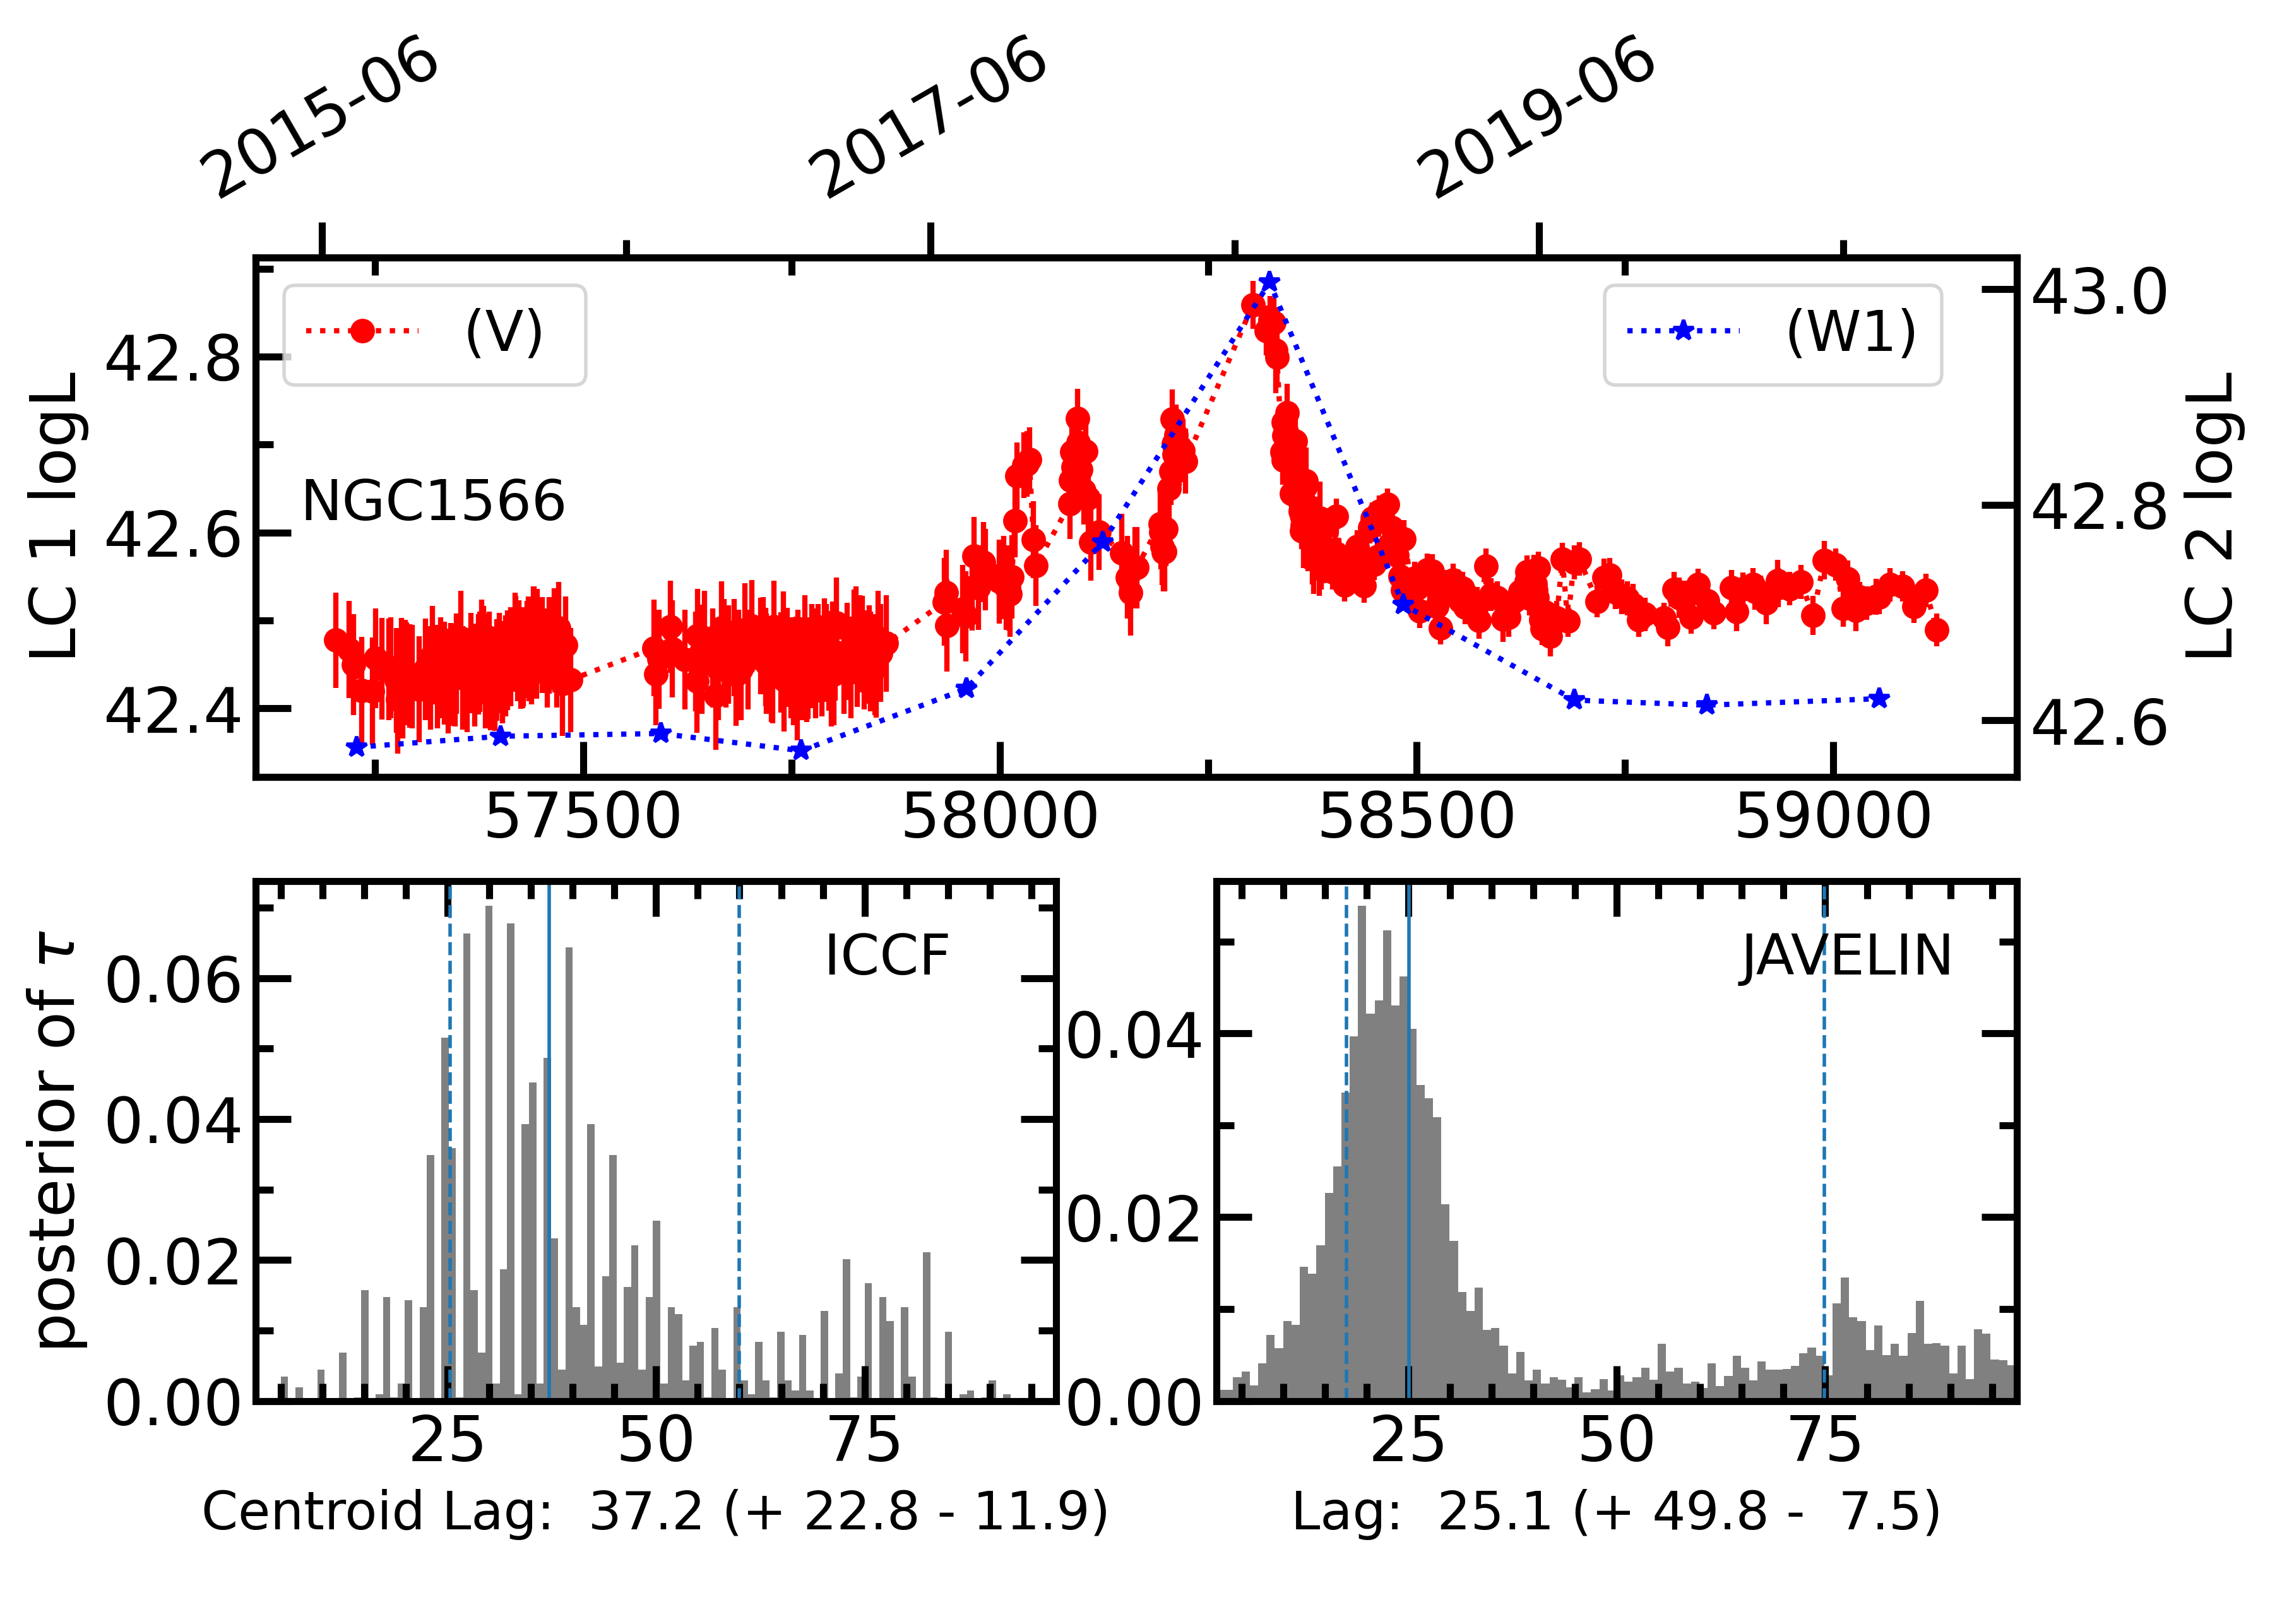
\includegraphics[width=0.5\textwidth]{pic/NGC1566_lag.png}
    \caption{Dust-reverberation time lag analysis for NGC 1566. }
    \label{fig:lag_NGC1566}
\end{figure}

For other sources, we only use the V band data from ASAS-SN and the re-binned $W1$ data in each visit with good observational overlaps to estimate the time lags. For Mrk 6 and PG1535+547, the V band data are binned in 30 days due to their complex short-term variability. The detailed time lag analysis are similar to NGC 1566. The results from ICCF and {\sc javelin} method are roughly consistent (see Figure 7--15), though the ICCF method almost yields a larger errorbar. 


\begin{figure}
\centering
	% To include a figure from a file named example.*
	% Allowable file formats are eps or ps if compiling using latex
	% or pdf, png, jpg if compiling using pdflatex
	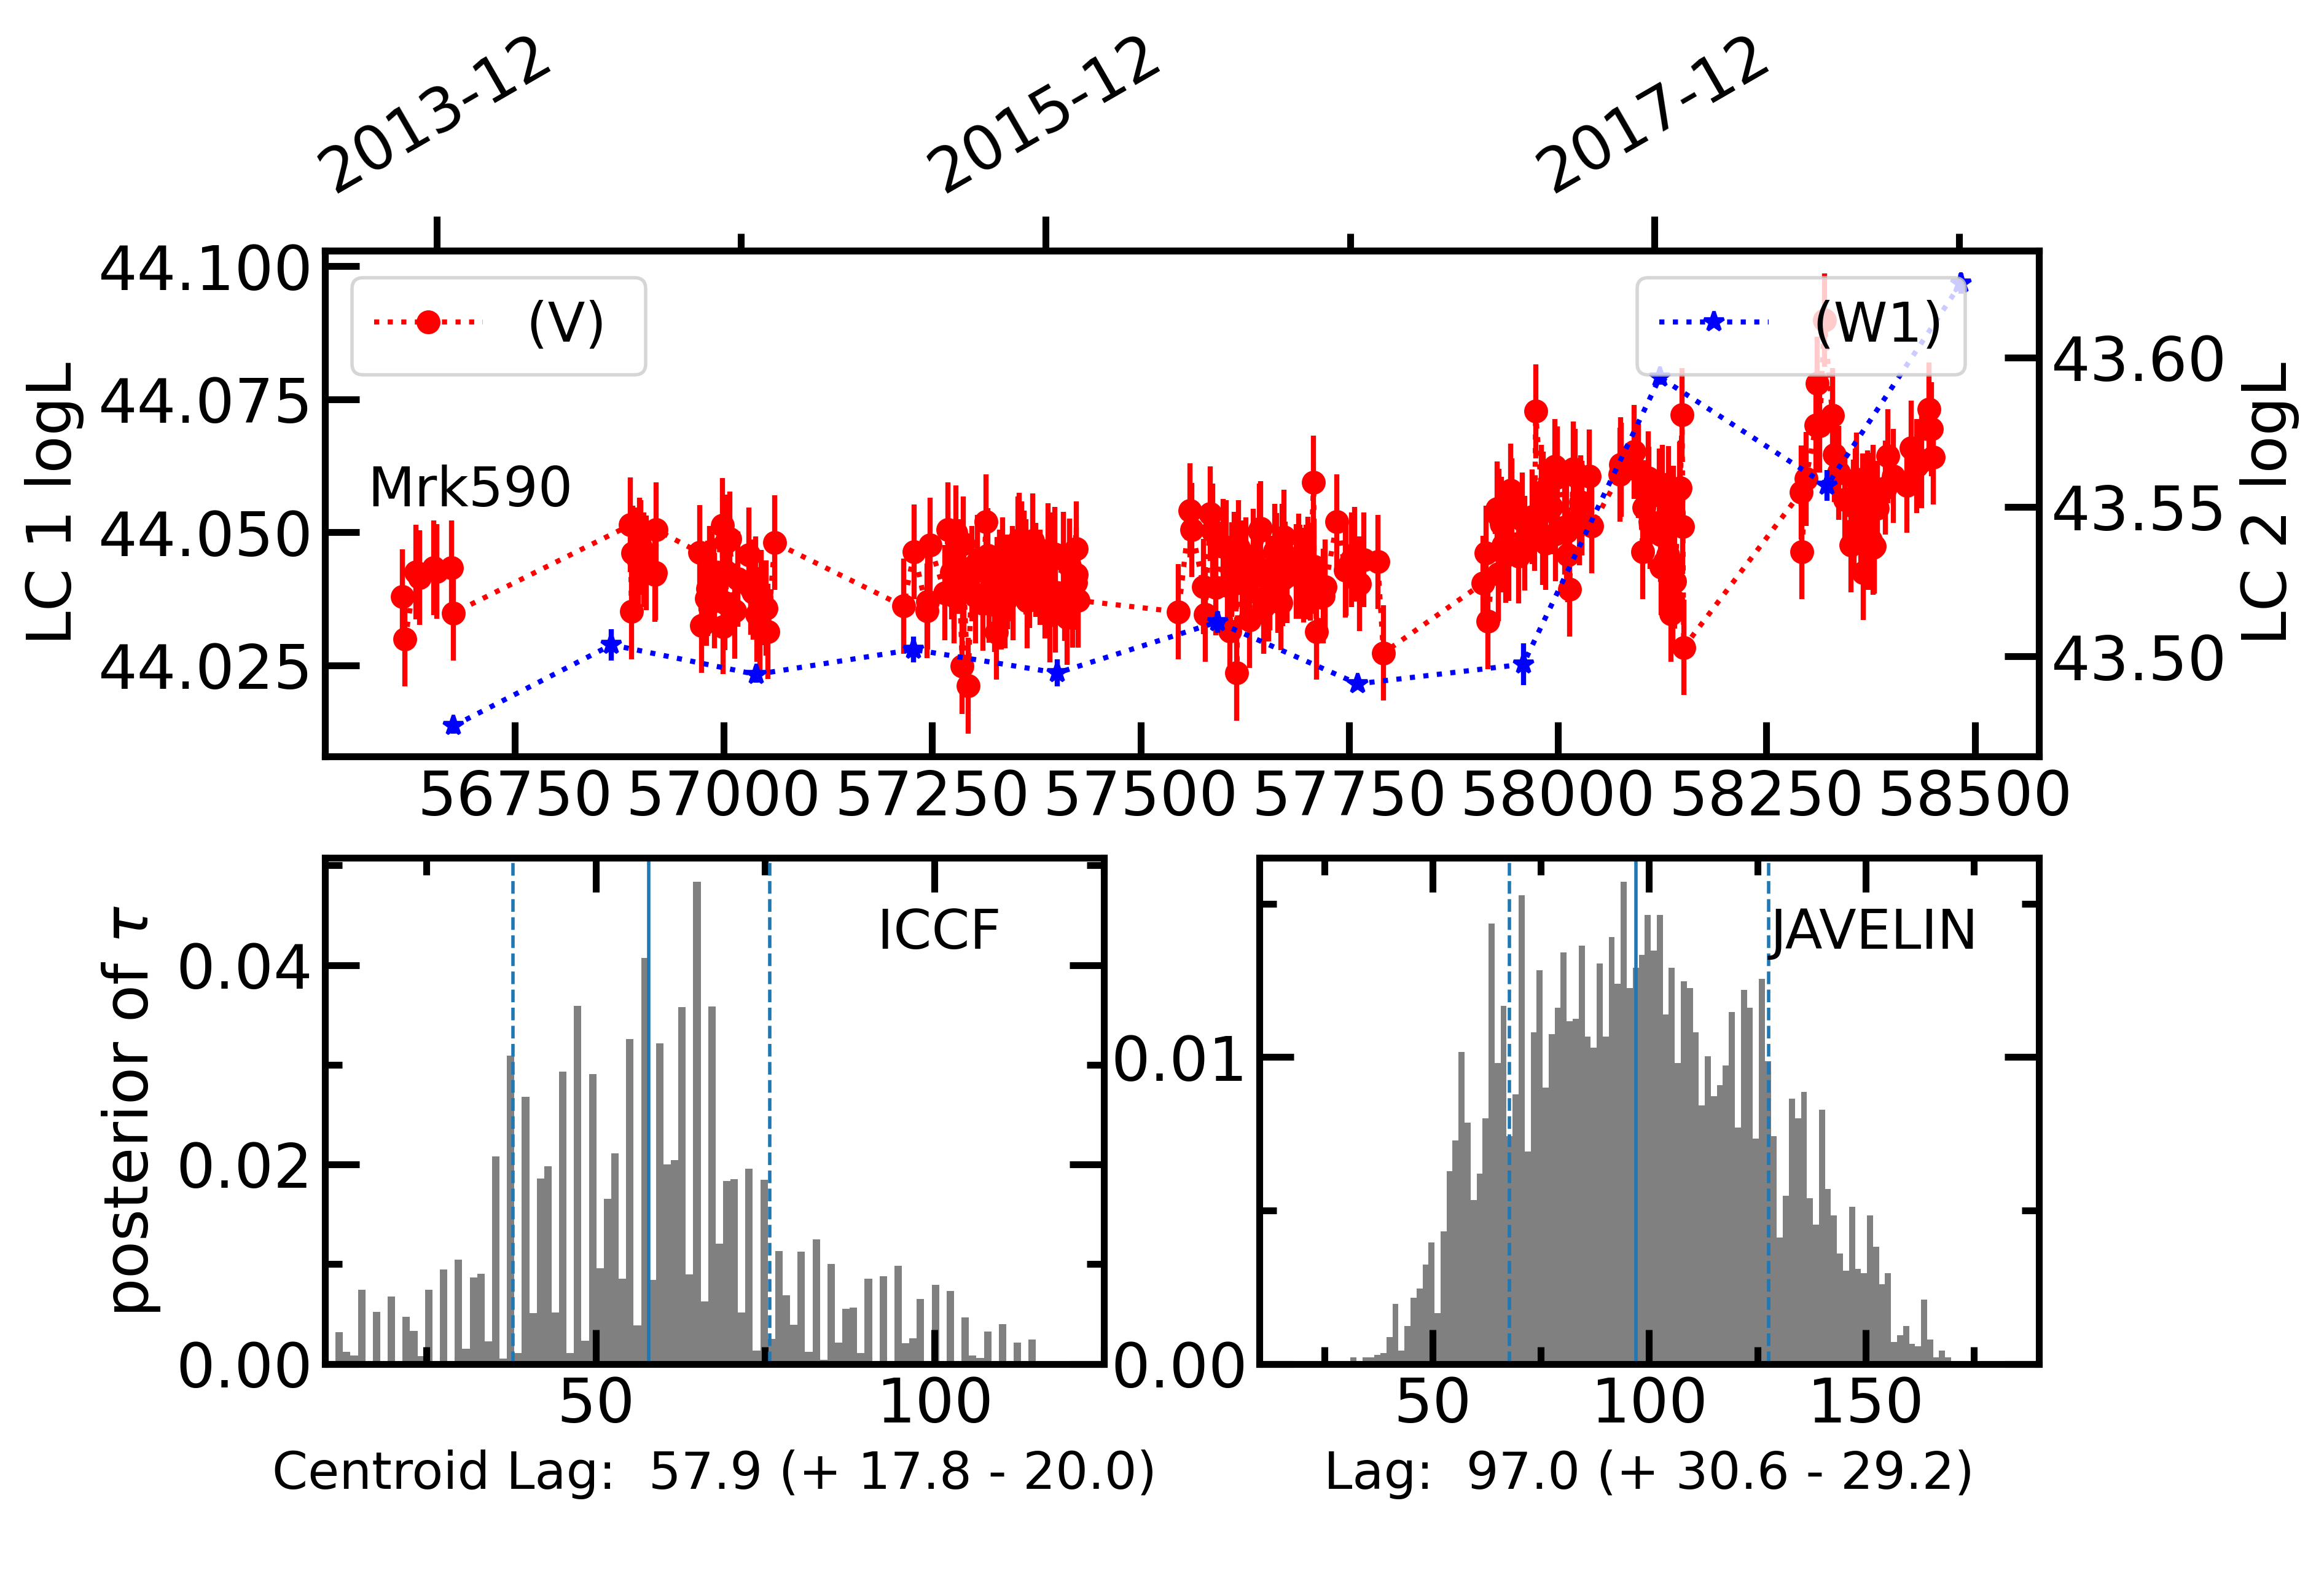
\includegraphics[width=0.5\textwidth]{pic/Mrk590lag.png}
    \caption{Dust-reverberation time lag analysis for Mrk 590. }
    \label{fig:lag_Mrk590}
\end{figure}
\begin{figure}
\centering
	% To include a figure from a file named example.*
	% Allowable file formats are eps or ps if compiling using latex
	% or pdf, png, jpg if compiling using pdflatex
	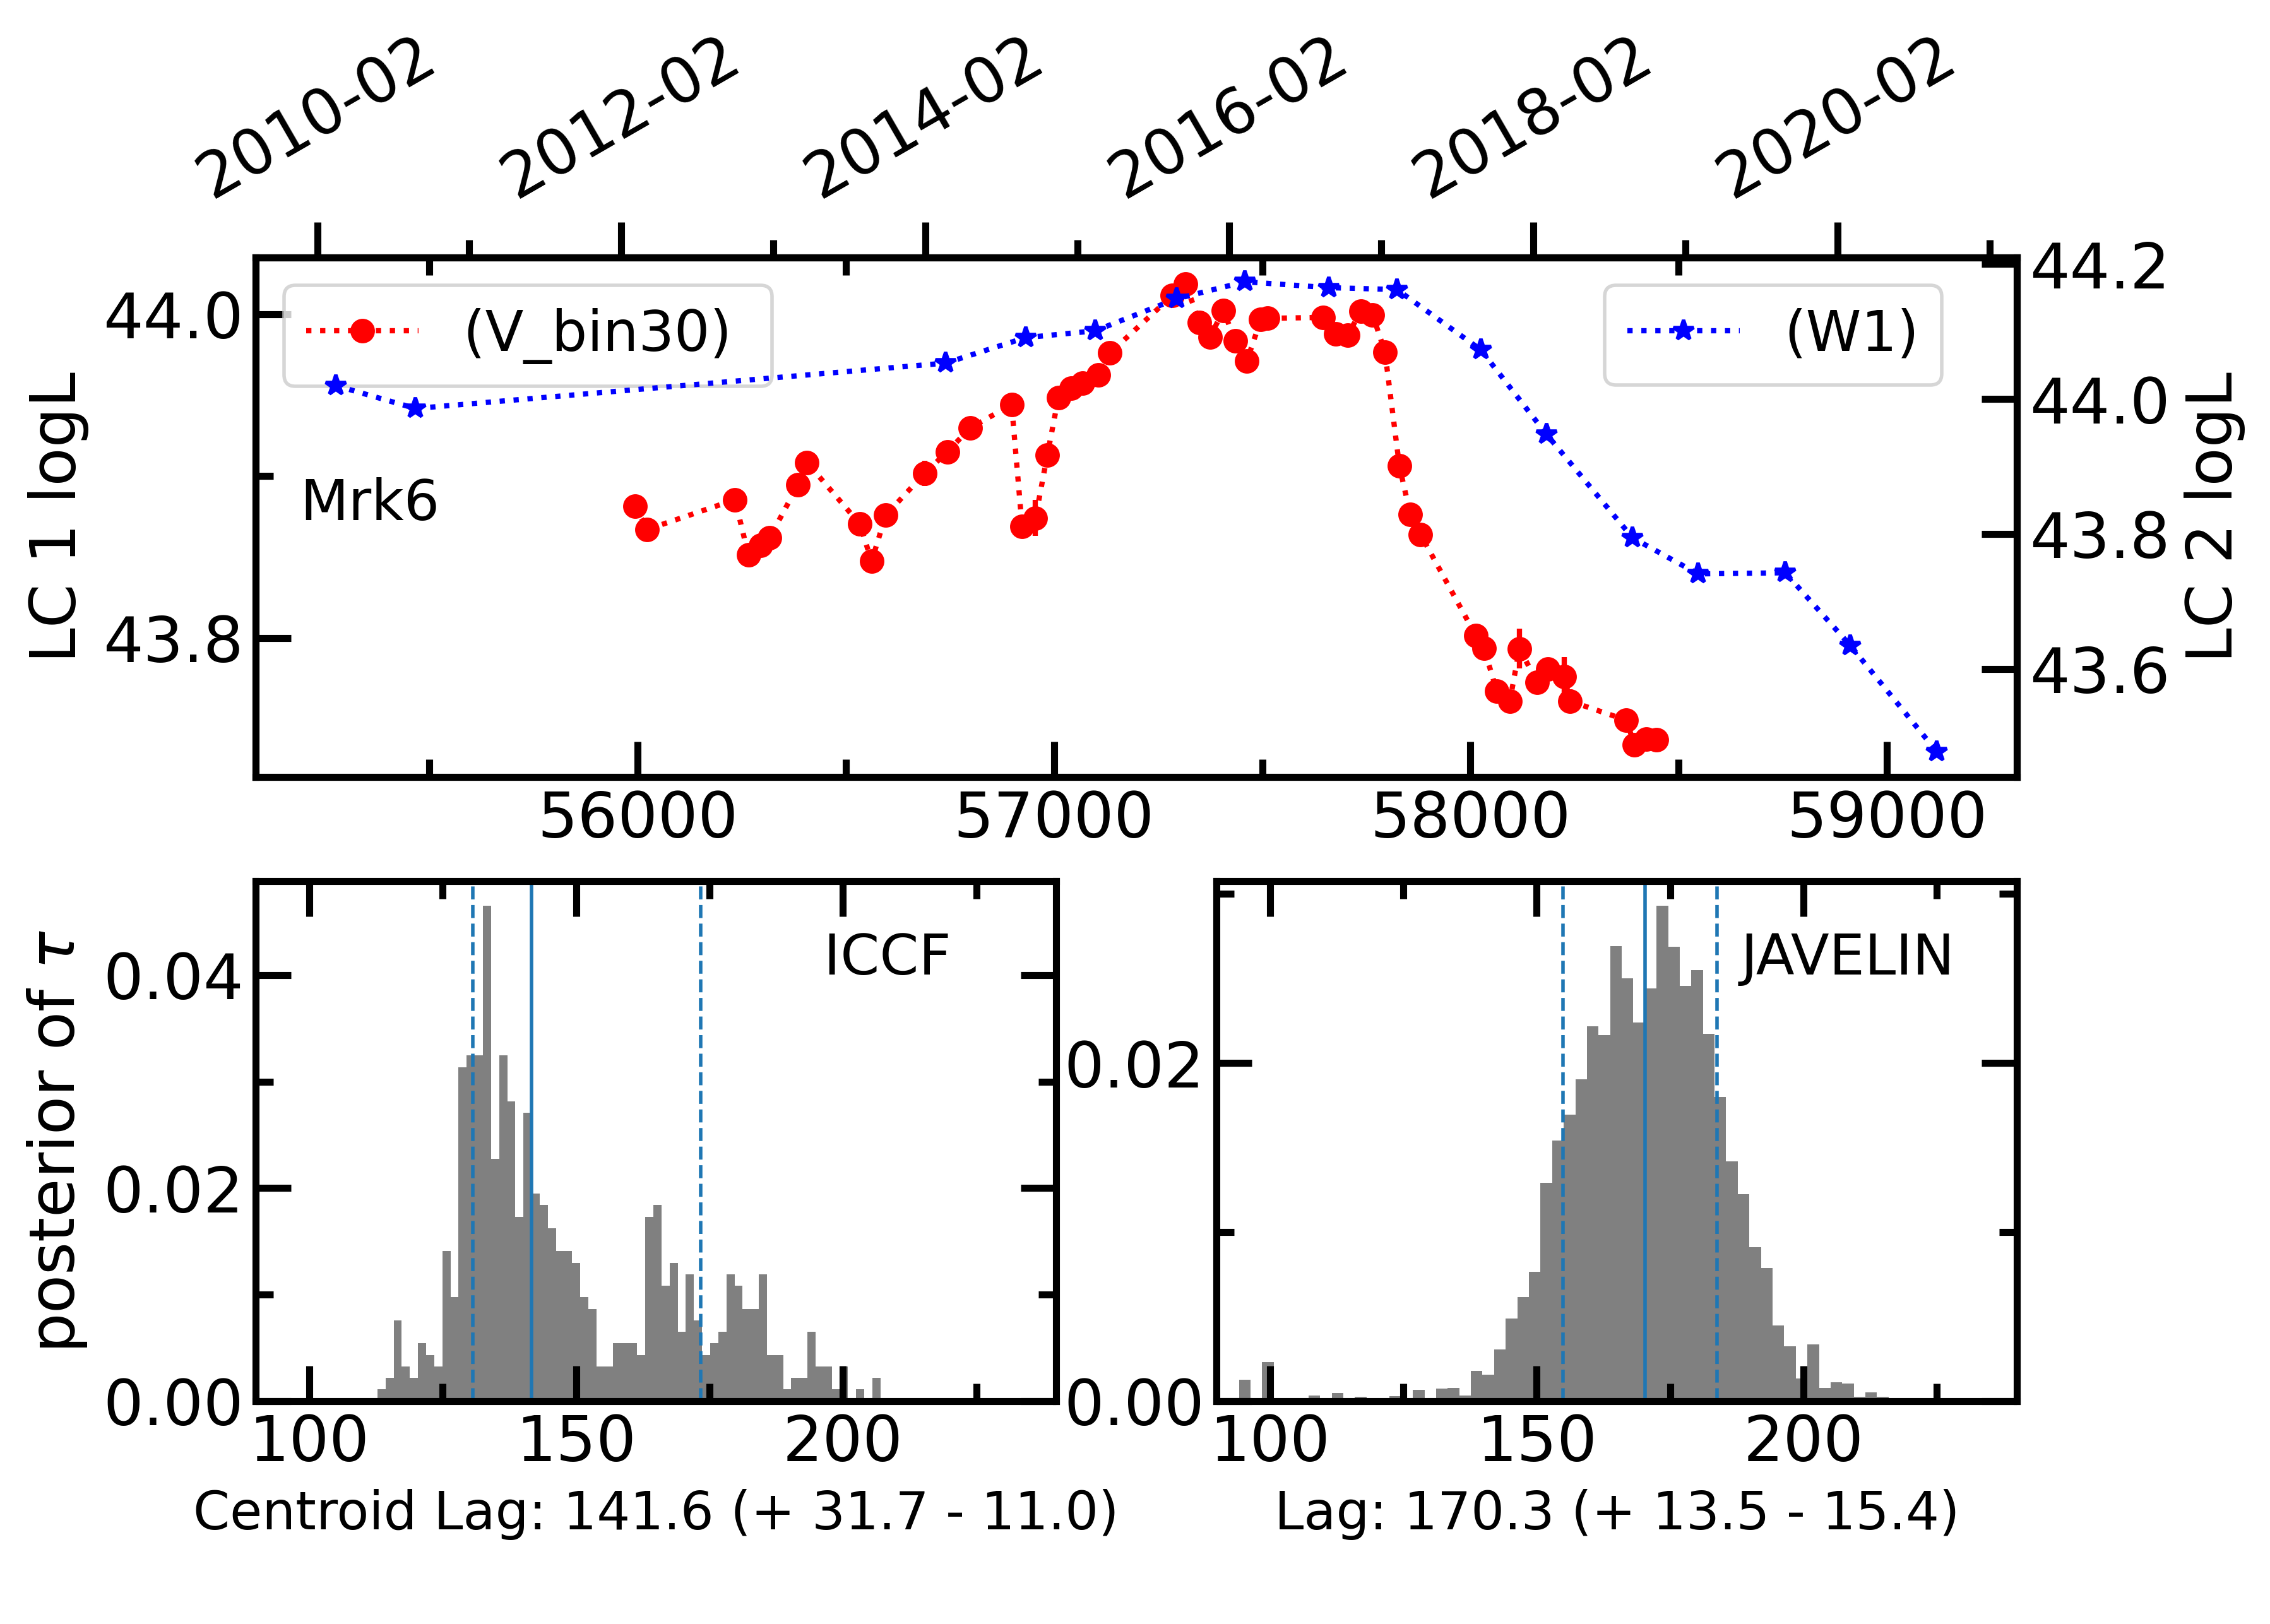
\includegraphics[width=0.5\textwidth]{pic/Mrk6lag1.png}
    \caption{Dust-reverberation time lag analysis for Mrk 6. }
    \label{fig:lag_Mrk6}
\end{figure}
\begin{figure}
\centering
	% To include a figure from a file named example.*
	% Allowable file formats are eps or ps if compiling using latex
	% or pdf, png, jpg if compiling using pdflatex
	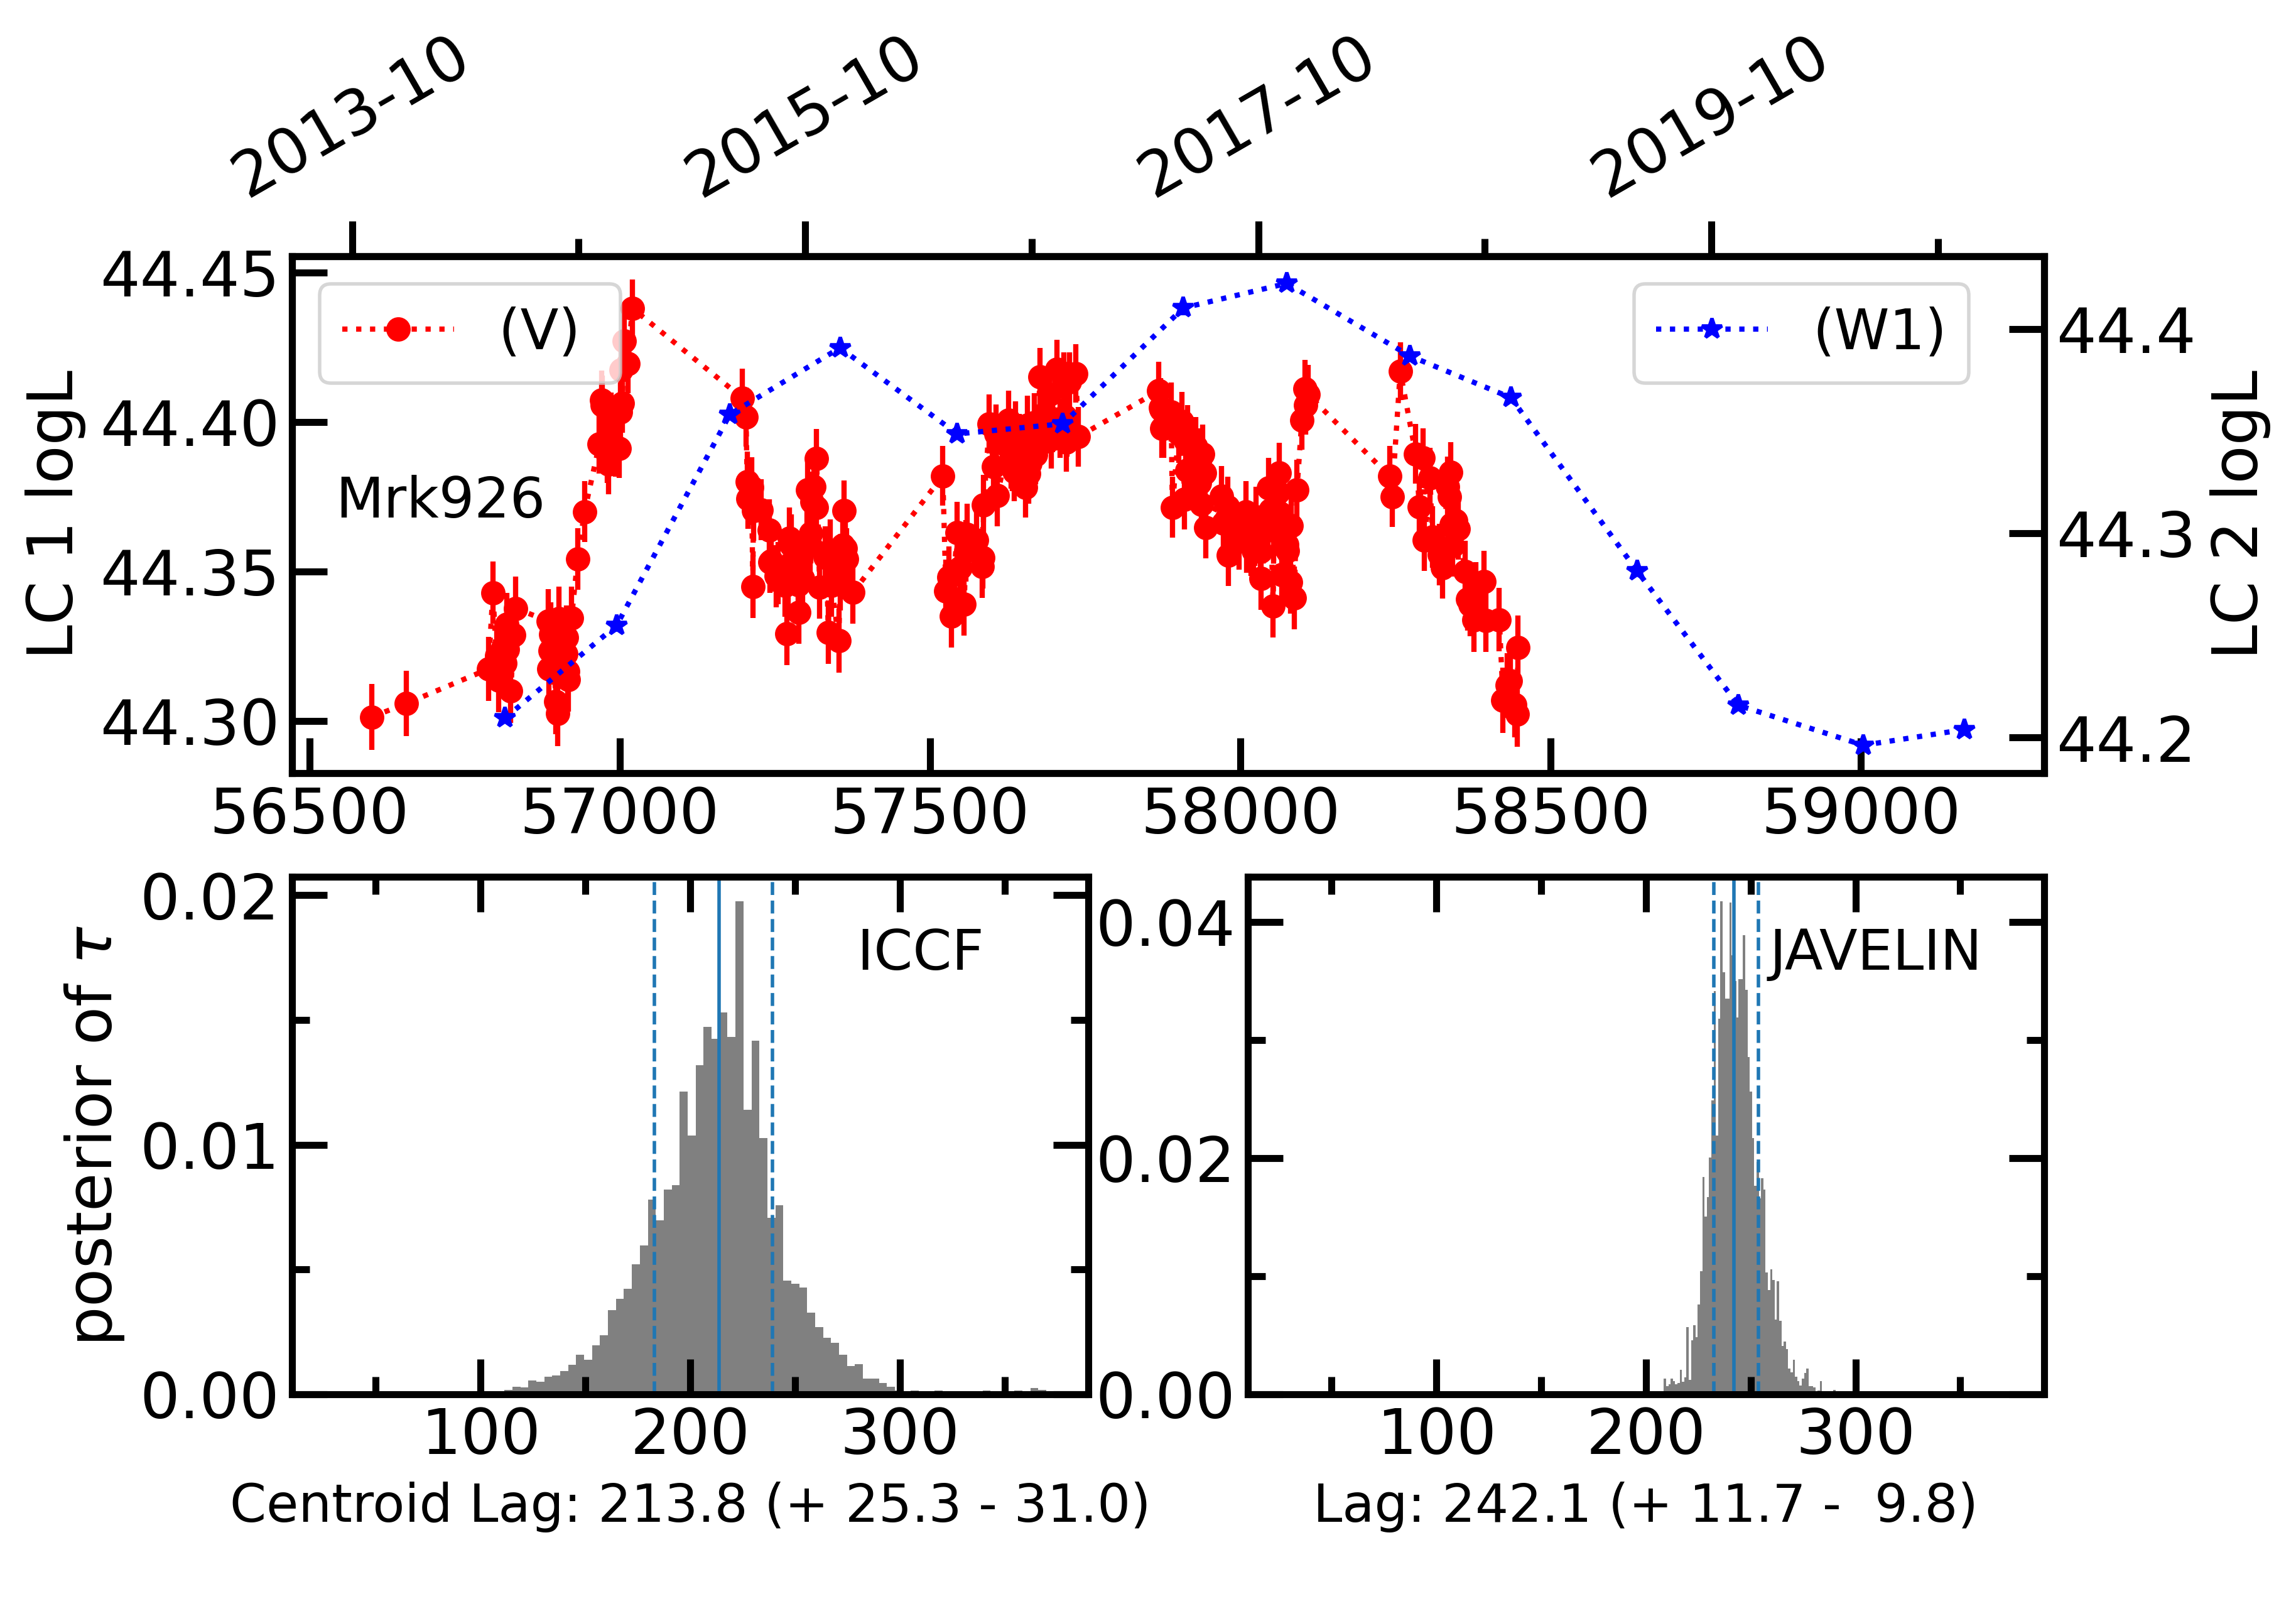
\includegraphics[width=0.5\textwidth]{pic/Mrk926lag.png}
    \caption{Dust-reverberation time lag analysis for Mrk 926. }
    \label{fig:lag_Mrk926}
\end{figure}




\begin{figure}
\centering
	% To include a figure from a file named example.*
	% Allowable file formats are eps or ps if compiling using latex
	% or pdf, png, jpg if compiling using pdflatex
	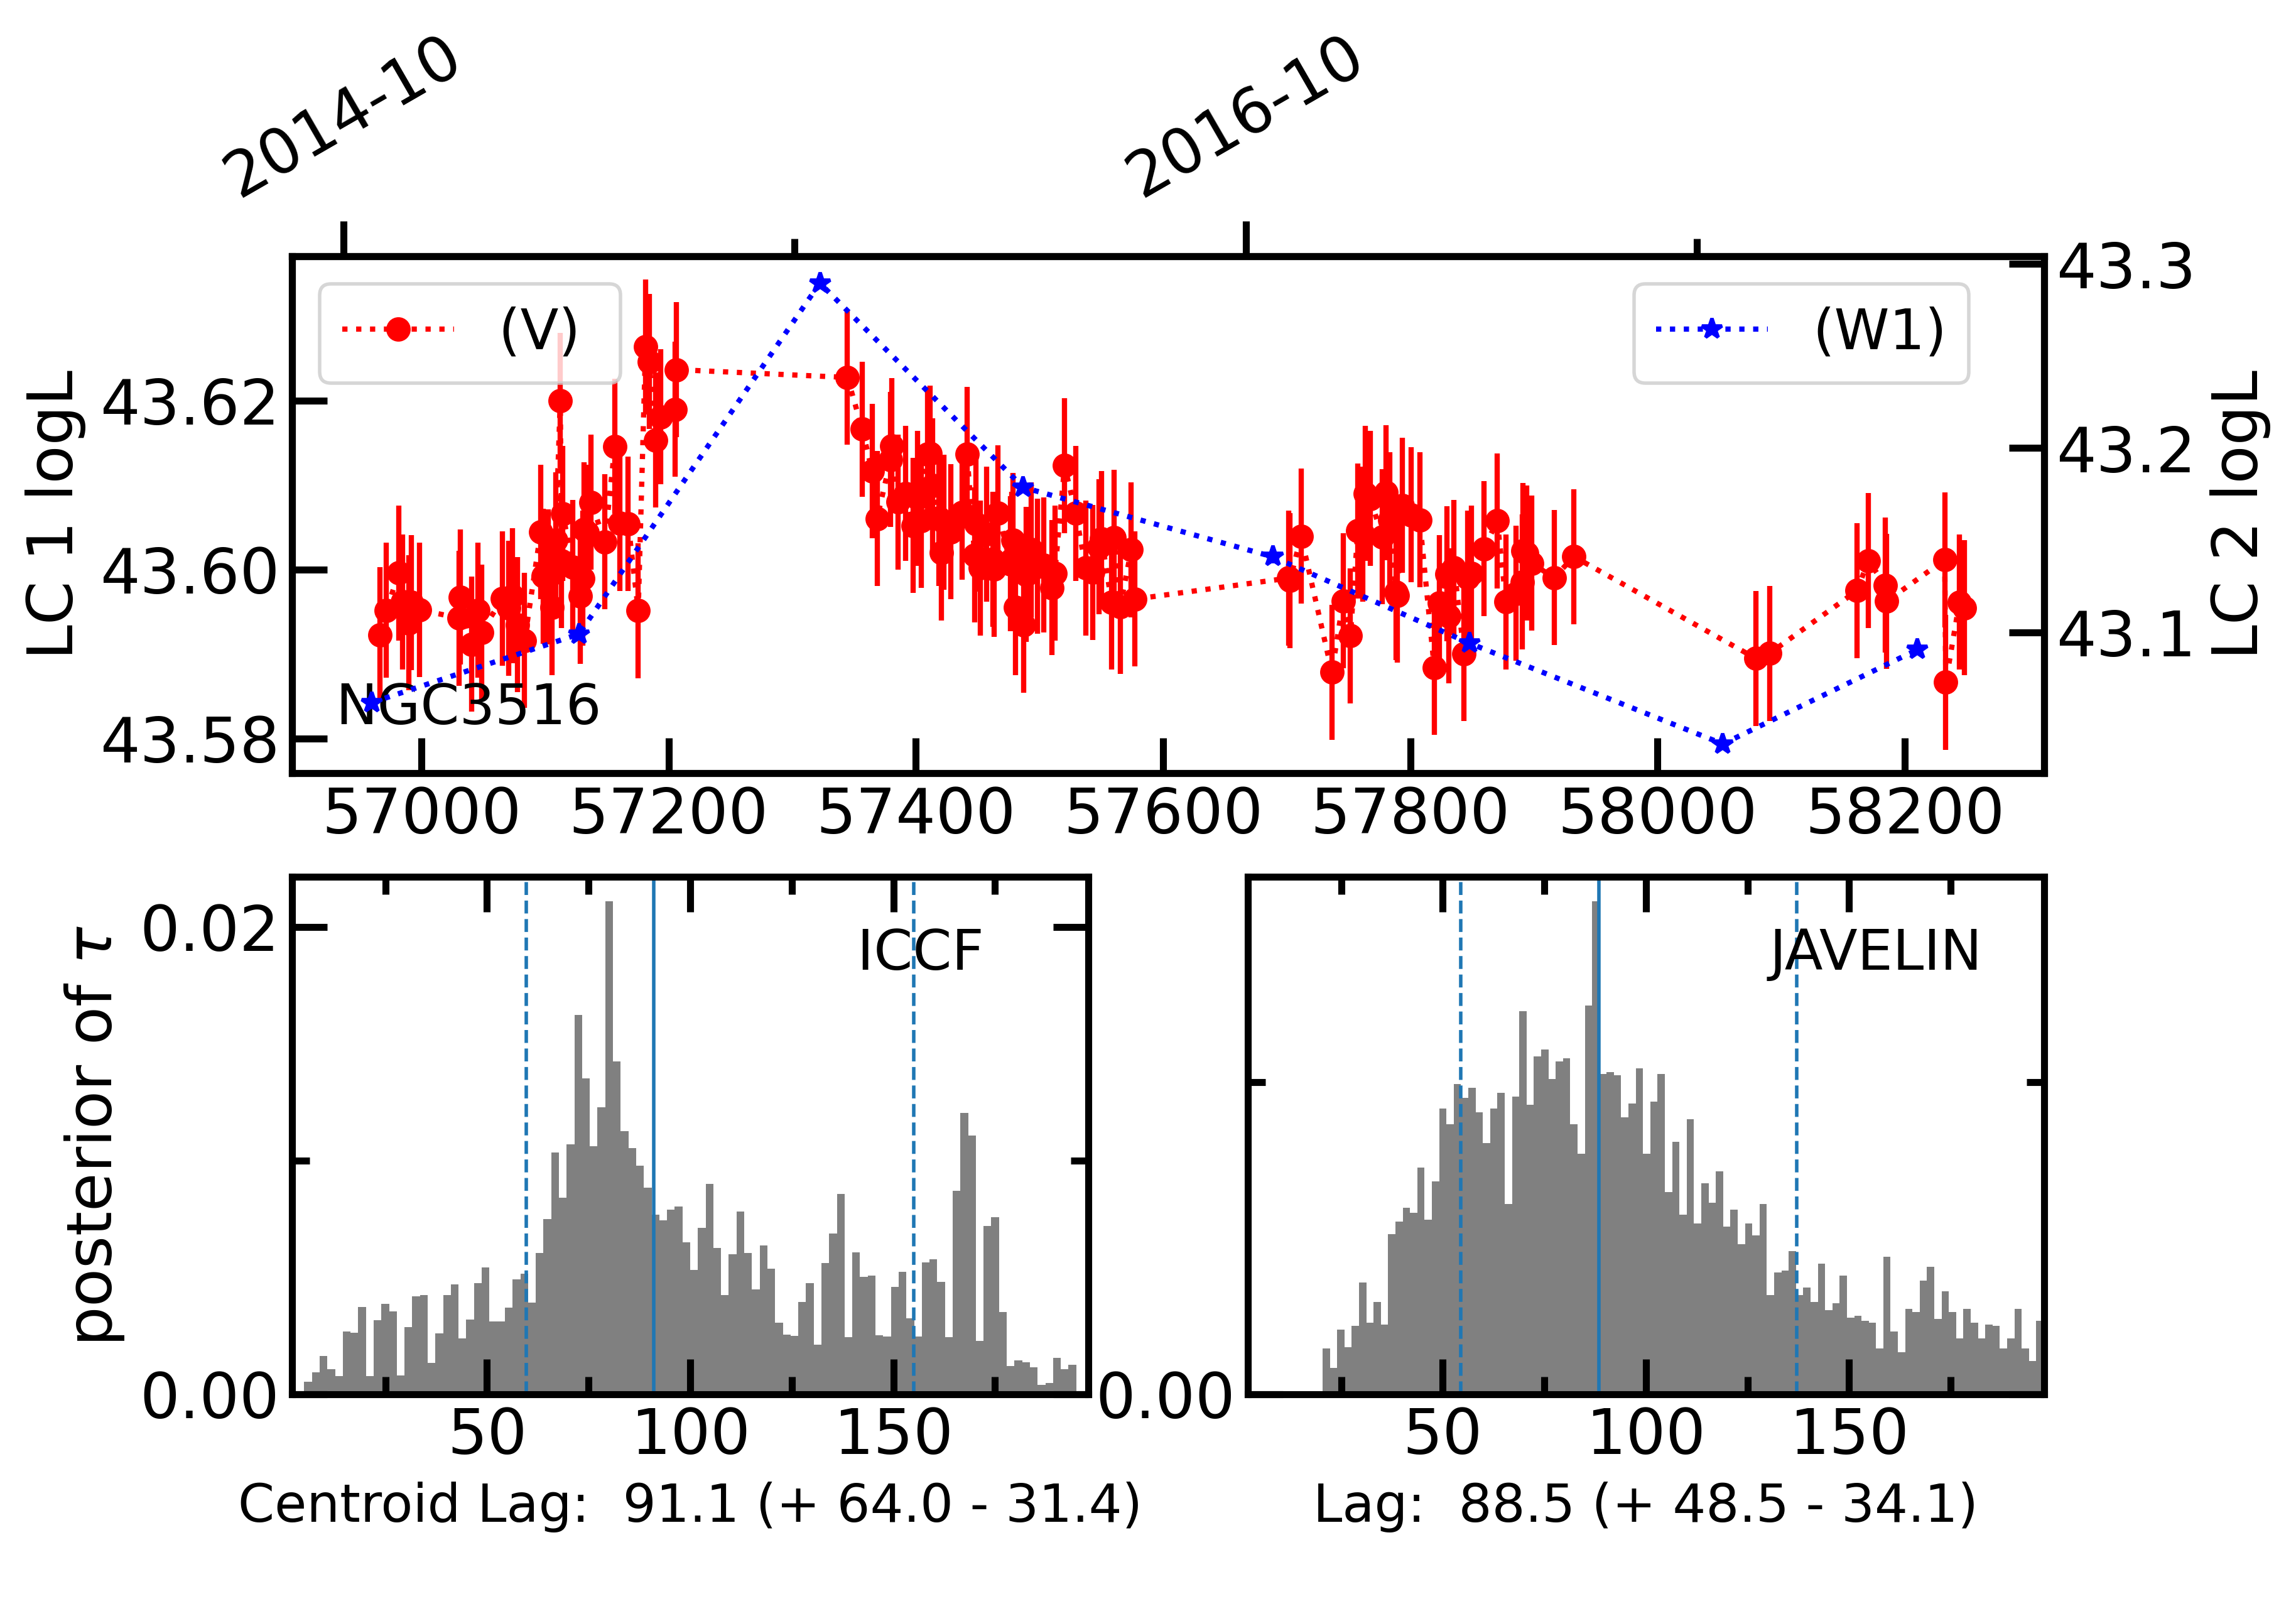
\includegraphics[width=0.5\textwidth]{pic/NGC3516lag.png}
    \caption{Dust-reverberation time lag analysis for NGC 3516. }
    \label{fig:lag_NGC3516}
\end{figure}

\begin{figure}
\centering
	% To include a figure from a file named example.*
	% Allowable file formats are eps or ps if compiling using latex
	% or pdf, png, jpg if compiling using pdflatex
	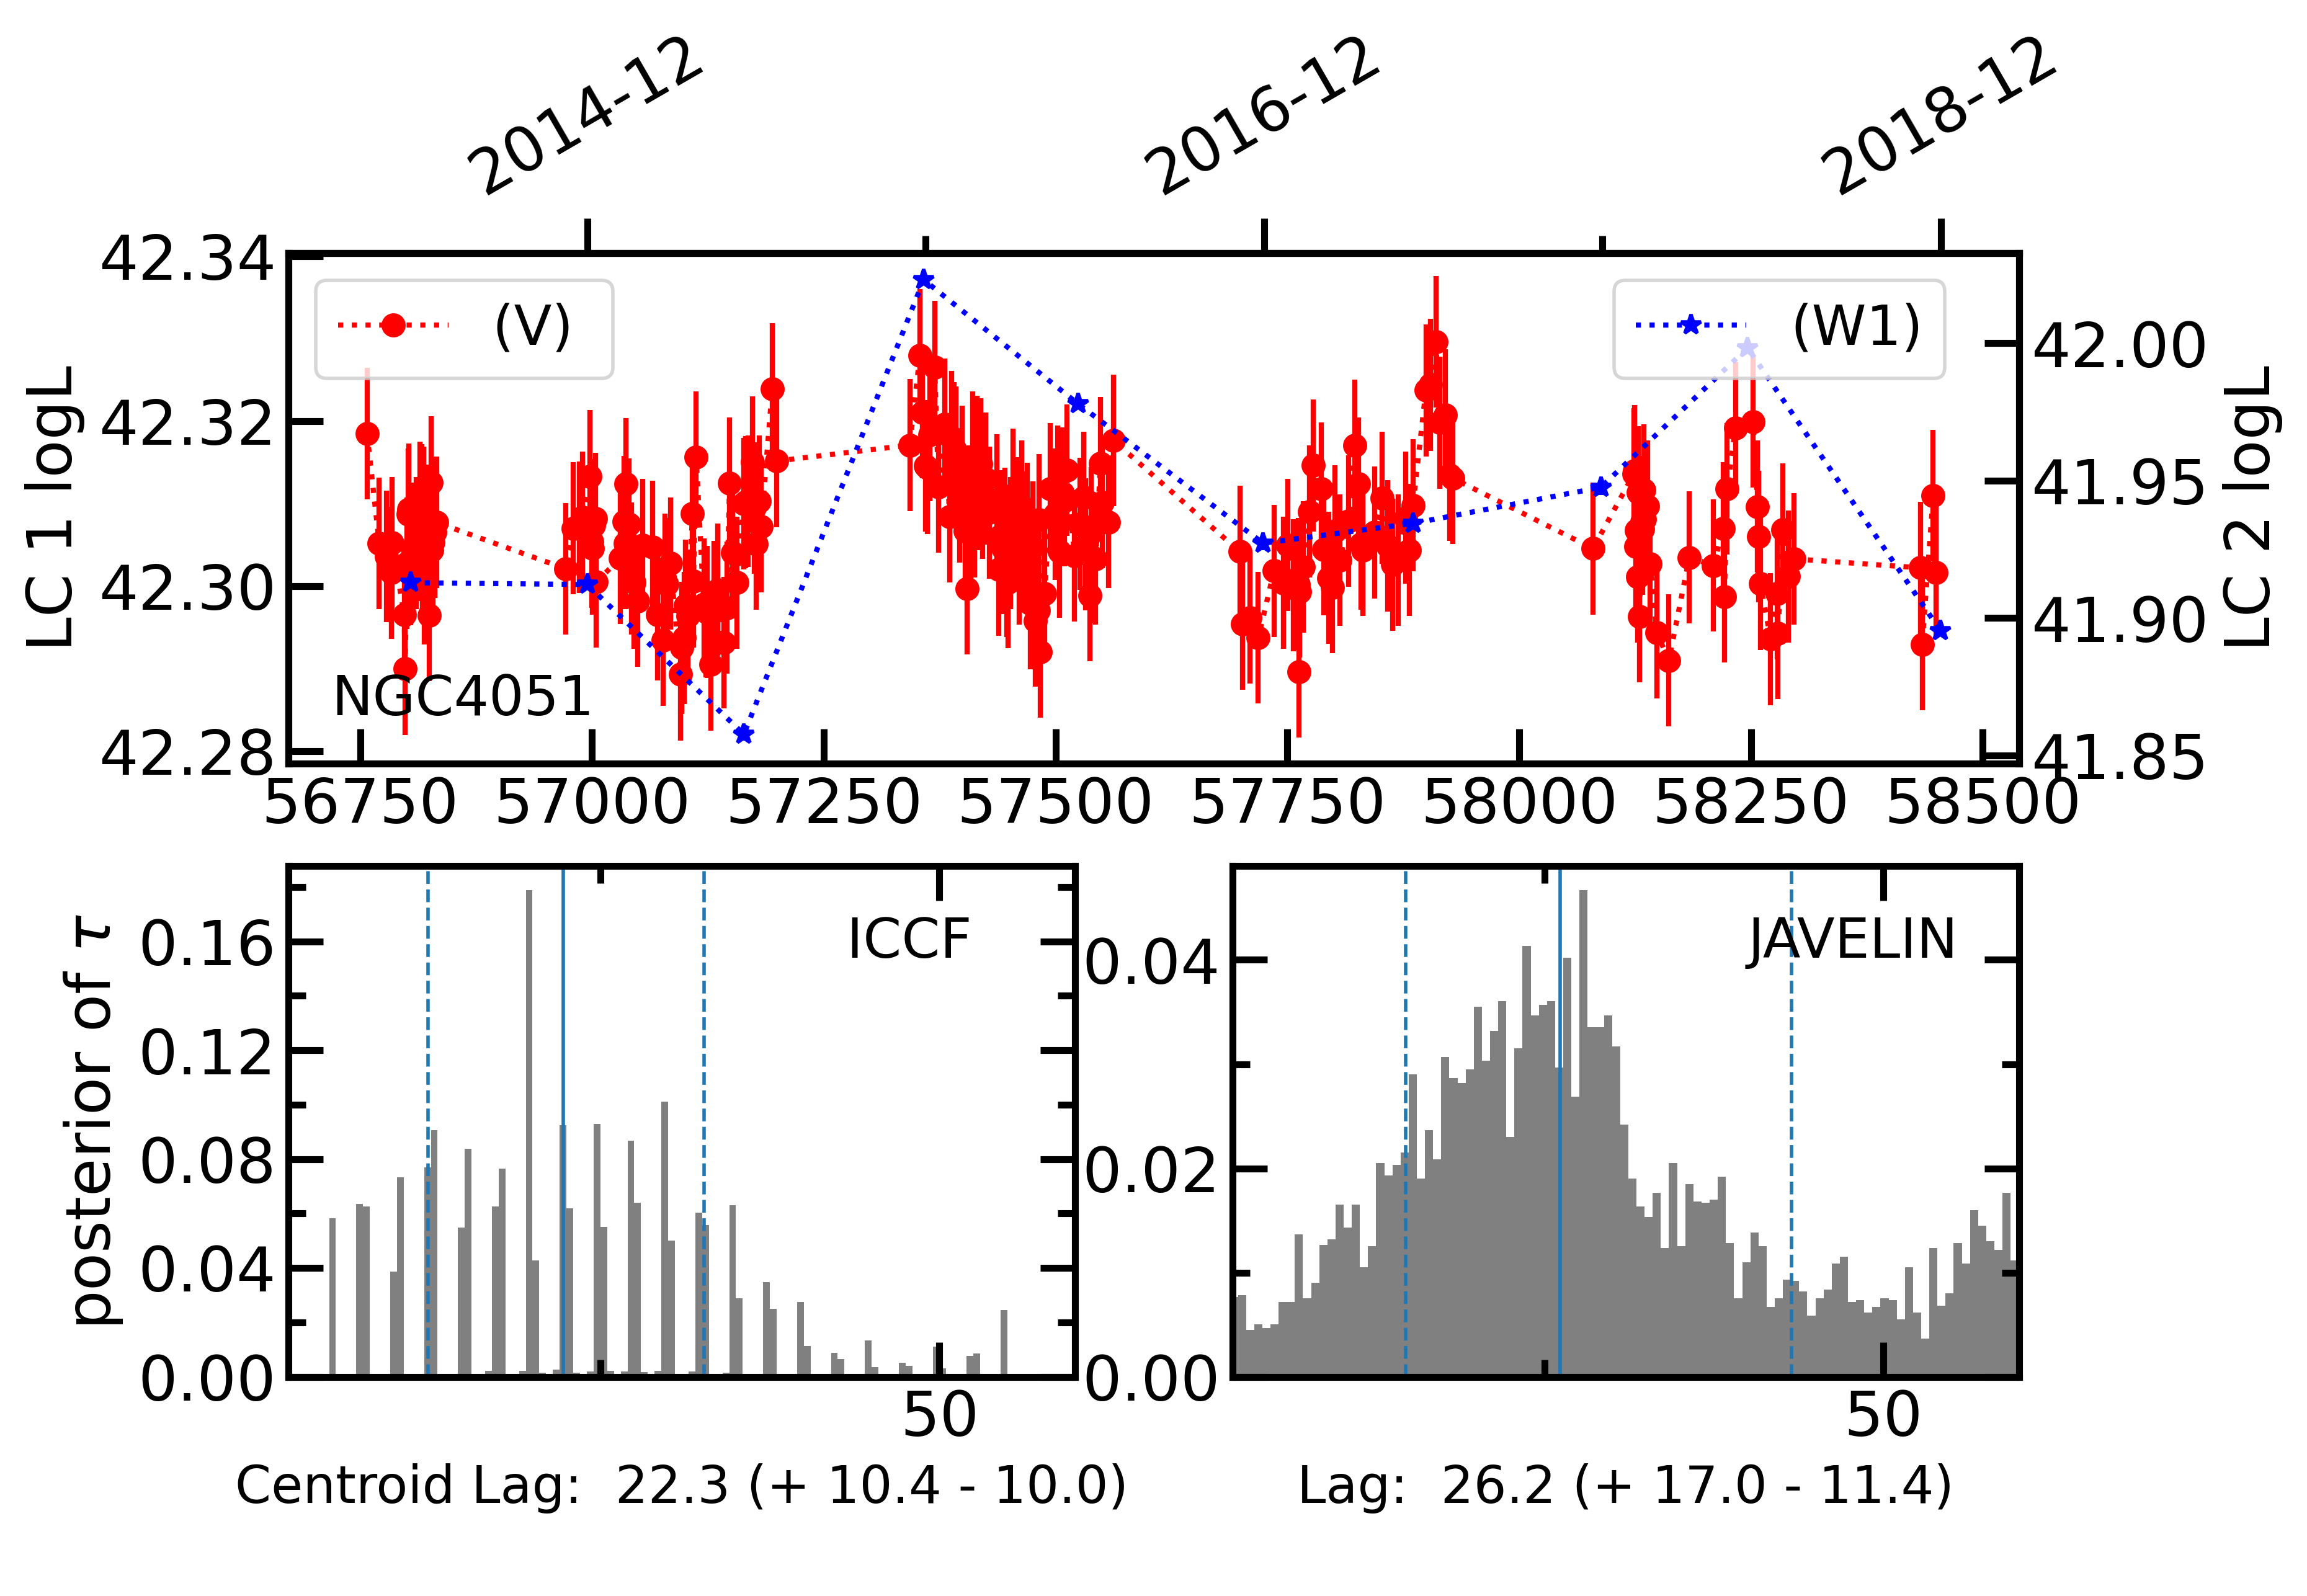
\includegraphics[width=0.5\textwidth]{pic/NGC4051lag.png}
    \caption{Dust-reverberation time lag analysis for NGC 4051. }
    \label{fig:lag_NGC4051}
\end{figure}

\begin{figure}
\centering
	% To include a figure from a file named example.*
	% Allowable file formats are eps or ps if compiling using latex
	% or pdf, png, jpg if compiling using pdflatex
	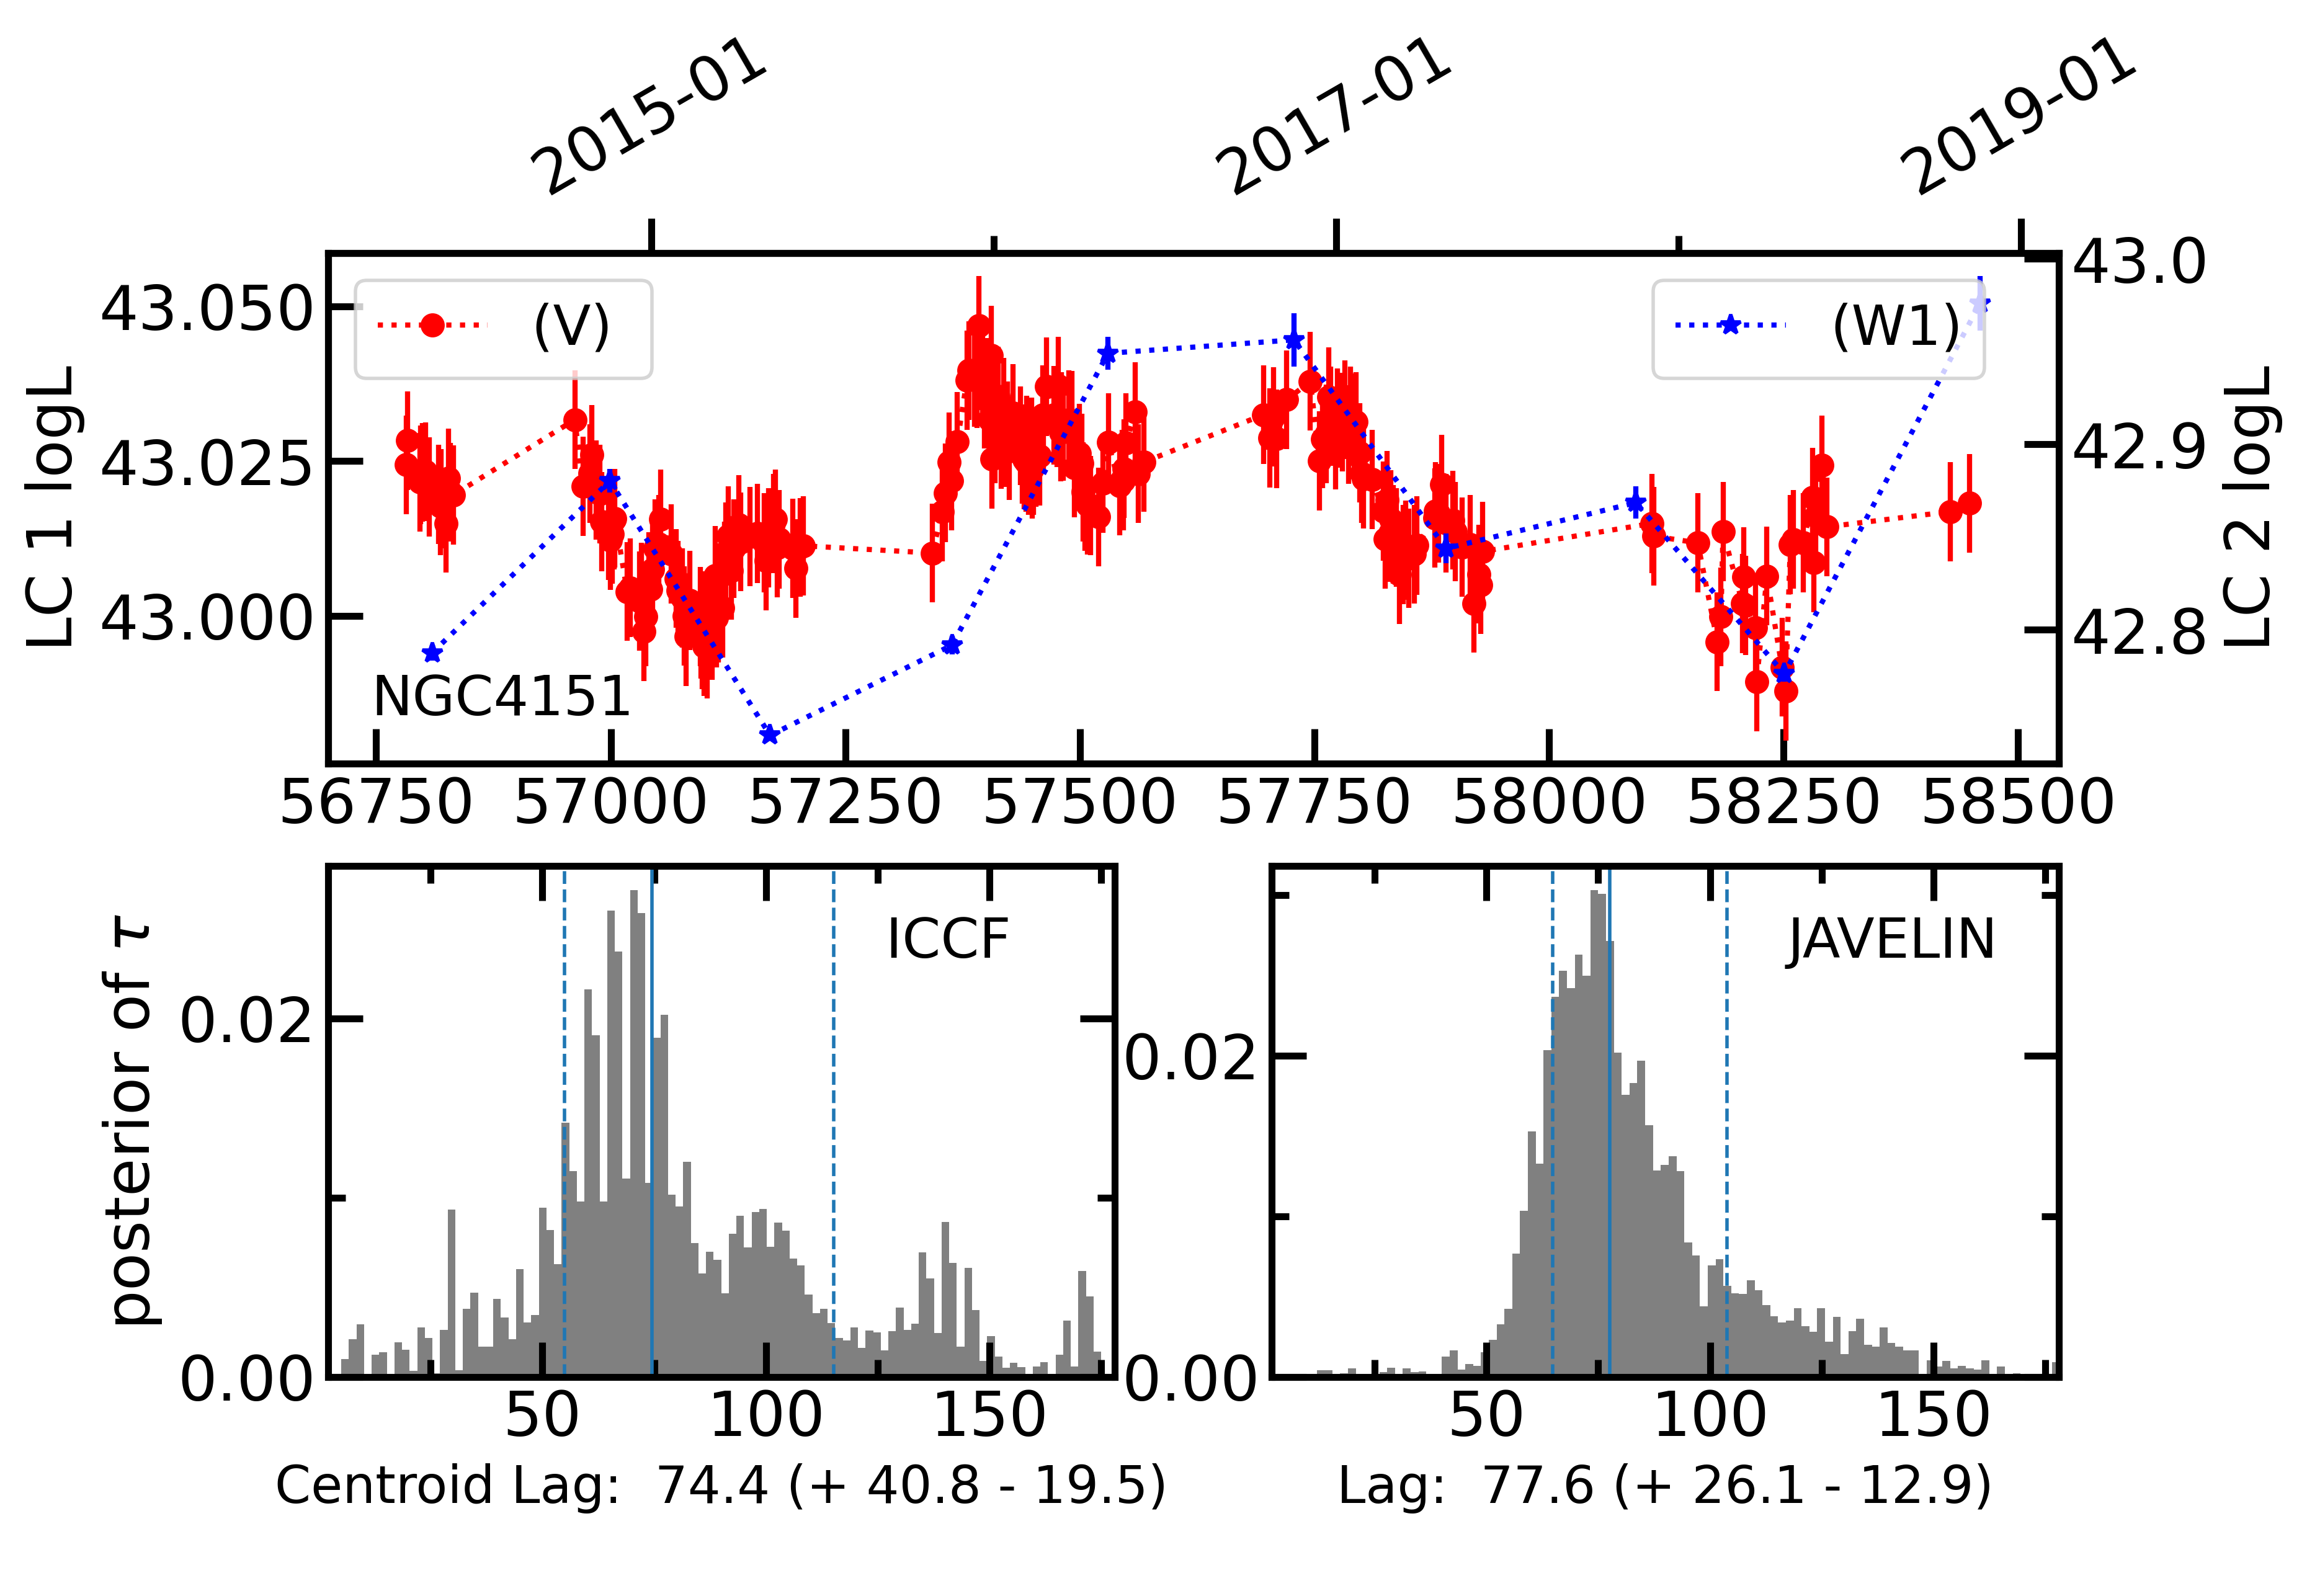
\includegraphics[width=0.5\textwidth]{pic/NGC4151lag.png}
    \caption{Dust-reverberation time lag analysis for NGC 4151. }
    \label{fig:lag_NGC4151}
\end{figure}

\begin{figure}
\centering
	% To include a figure from a file named example.*
	% Allowable file formats are eps or ps if compiling using latex
	% or pdf, png, jpg if compiling using pdflatex
	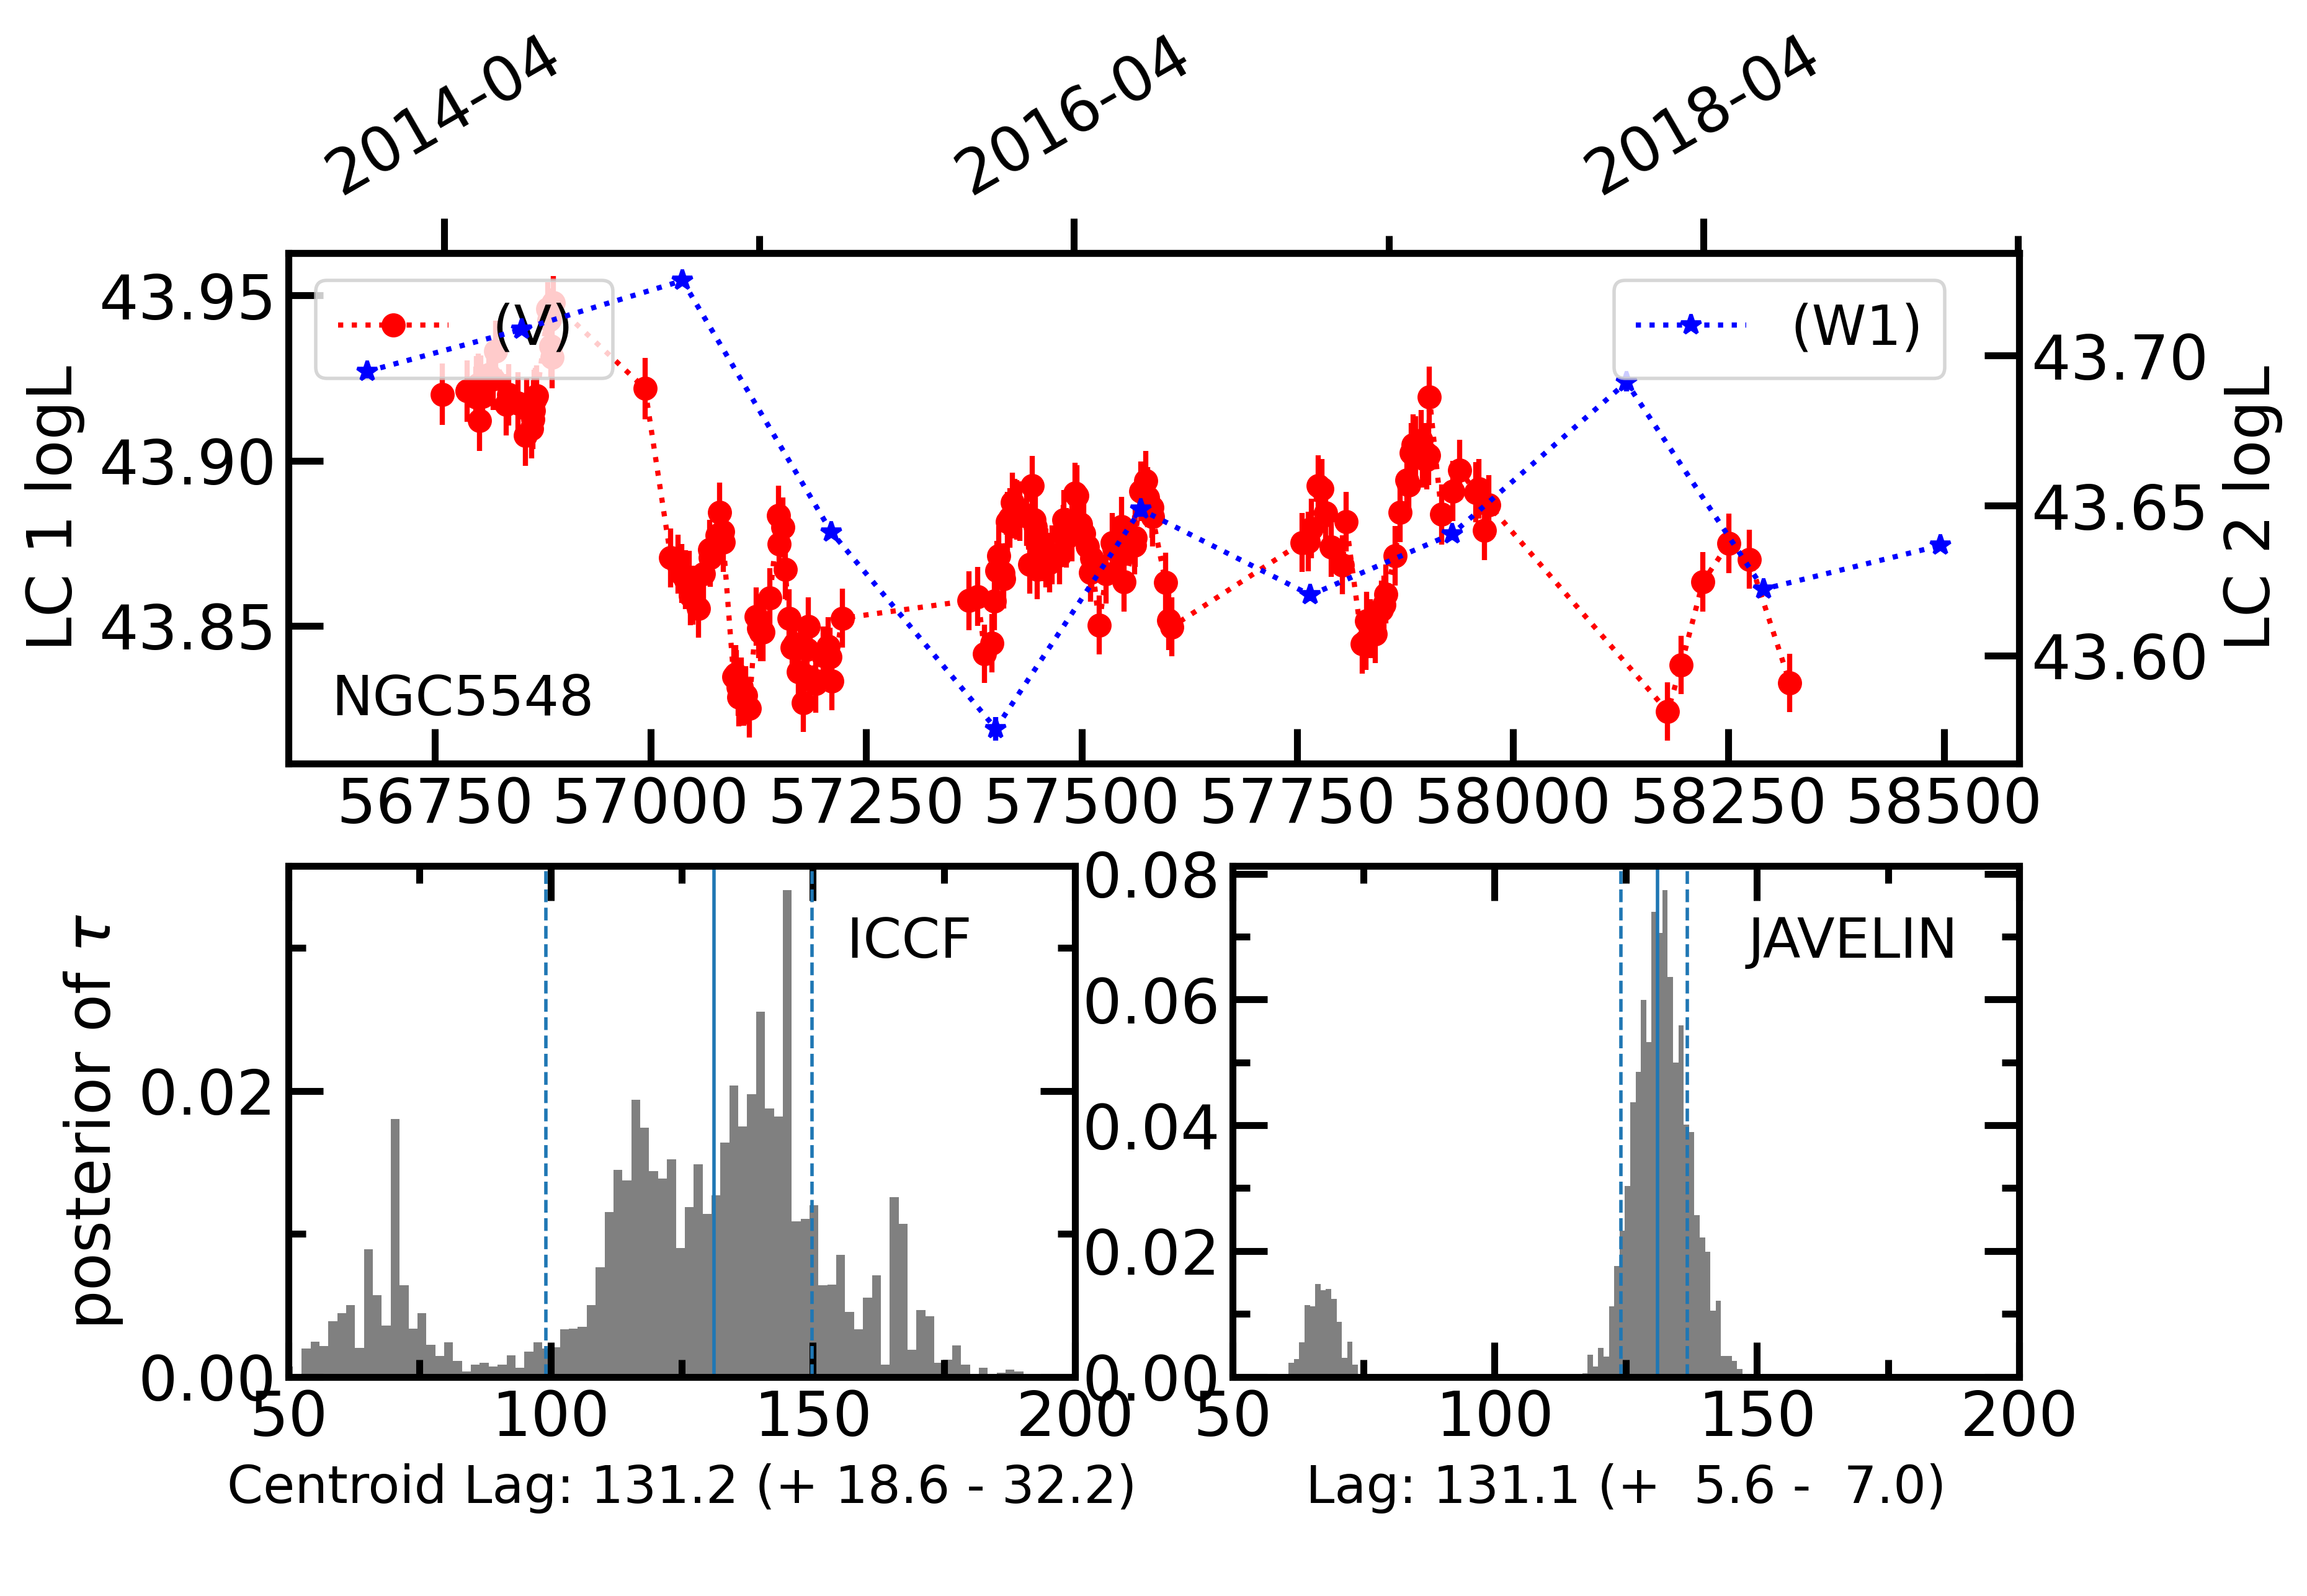
\includegraphics[width=0.5\textwidth]{pic/NGC5548lag.png}
    \caption{Dust-reverberation time lag analysis for NGC 5548. }
    \label{fig:lag_NGC5548}
\end{figure}

\begin{figure}
\centering
	% To include a figure from a file named example.*
	% Allowable file formats are eps or ps if compiling using latex
	% or pdf, png, jpg if compiling using pdflatex
	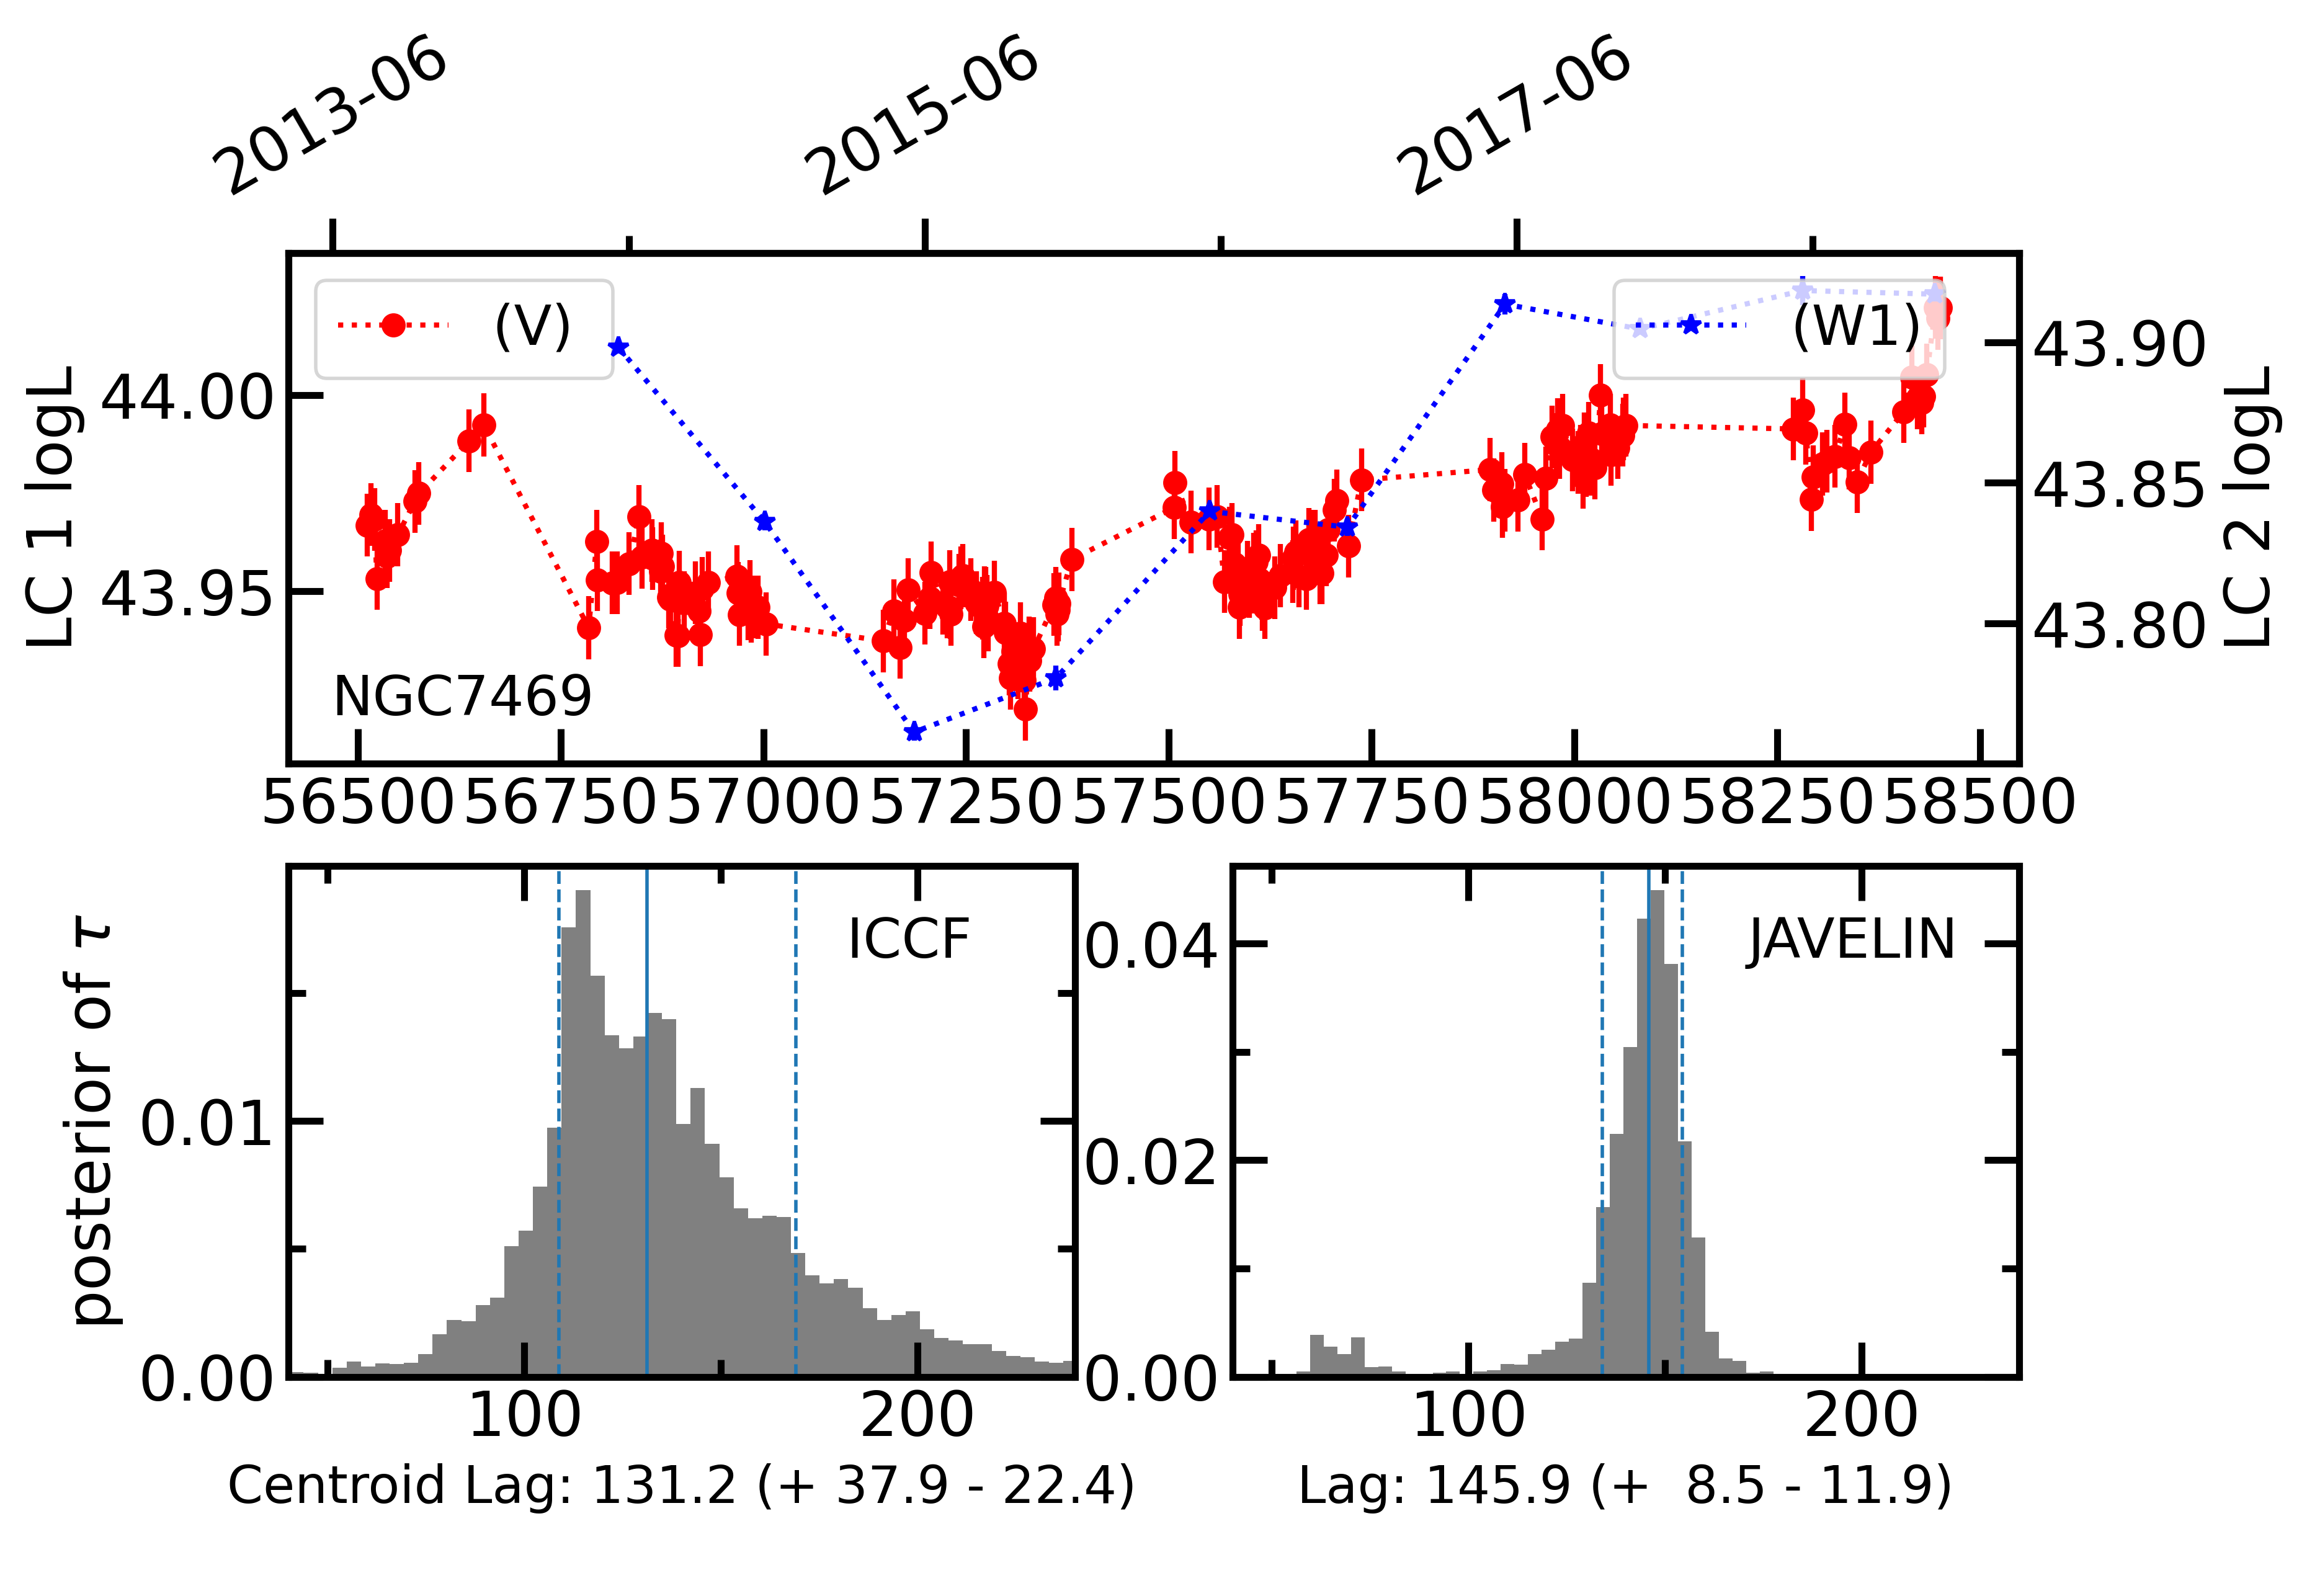
\includegraphics[width=0.5\textwidth]{pic/NGC7469lag.png}
    \caption{Dust-reverberation time lag analysis for NGC 7469. }
    \label{fig:lag_NGC7469}
\end{figure}
\begin{figure}
\centering
	% To include a figure from a file named example.*
	% Allowable file formats are eps or ps if compiling using latex
	% or pdf, png, jpg if compiling using pdflatex
	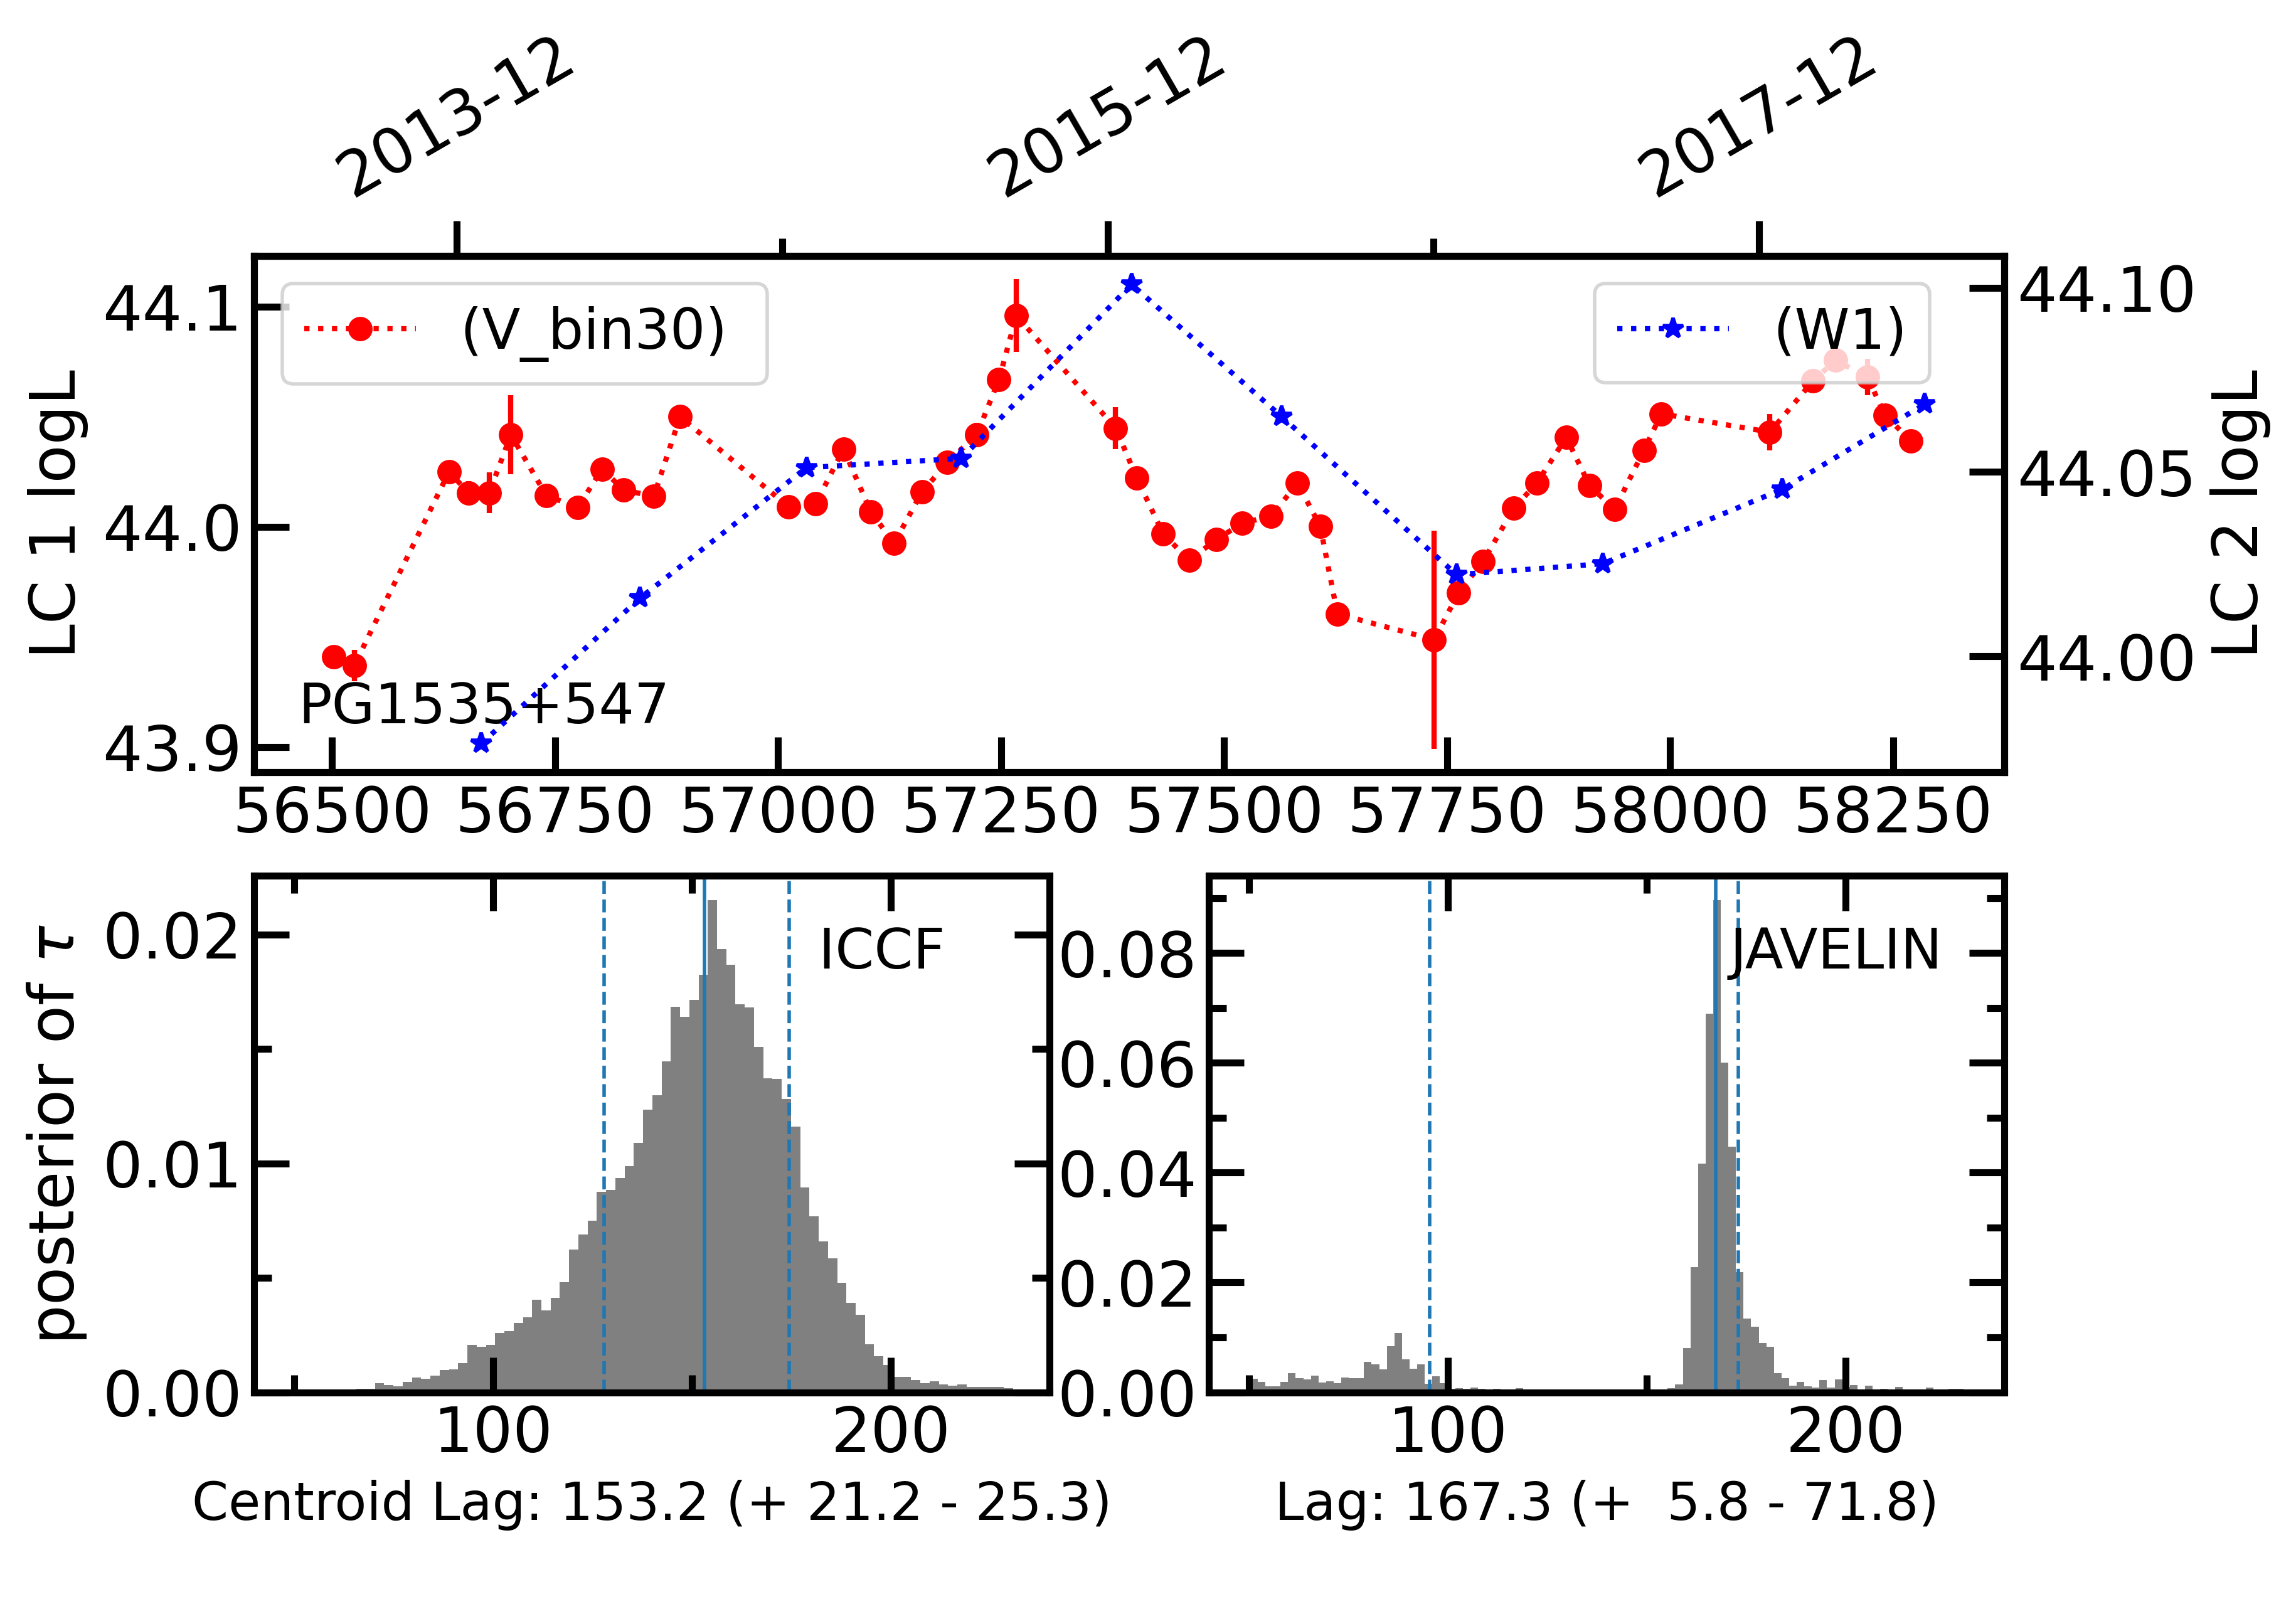
\includegraphics[width=0.5\textwidth]{pic/PG1535p547lag1.png}
    \caption{Dust-reverberation time lag analysis for PG 1535+547. }
    \label{fig:lag_PG1535}
\end{figure}



\end{document}

% End of file `sample631.tex'.



